%%%%%%%%%%%%%%%%%%%%%%%%%%%%%%%%%%%%%%%%%%%%%%%%%%%%%%%%%%%%%%%%%%%%%%%%%%%%%
%%%
%%% File: utthesis2.doc, version 2.0jab, February 2002
%%%
%%% Based on: utthesis.doc, version 2.0, January 1995
%%% =============================================
%%% Copyright (c) 1995 by Dinesh Das.  All rights reserved.
%%% This file is free and can be modified or distributed as long as
%%% you meet the following conditions:
%%%
%%% (1) This copyright notice is kept intact on all modified copies.
%%% (2) If you modify this file, you MUST NOT use the original file name.
%%%
%%% This file contains a template that can be used with the package
%%% utthesis.sty and LaTeX2e to produce a thesis that meets the requirements;
%%% of the Graduate School of The University of Texas at Austin.
%%%
%%% All of the commands defined by utthesis.sty have default values (see
%%% the file utthesis.sty for these values).  Thus, theoretically, you
%%% don't need to define values for any of them; you can run this file
%%% through LaTeX2e and produce an acceptable thesis, without any text.
%%% However, you probably want to set at least some of the macros (like
%%% \thesisauthor).  In that case, replace "..." with appropriate values,
%%% and uncomment the line (by removing the leading %'s).
%%%
%%%%%%%%%%%%%%%%%%%%%%%%%%%%%%%%%%%%%%%%%%%%%%%%%%%%%%%%%%%%%%%%%%%%%%%%%%%%%
%%% The style file was created for an American university, some information
%%% such as committee members, etc is not needed for TCD dissertations.

\documentclass[a4paper, 12pt, oneside]{report}

\usepackage {tcdthesis}             
\usepackage{graphicx,color}
\usepackage{anysize}
\usepackage{amsmath}
%\usepackage{natbib}
\usepackage{caption}
\usepackage{hyperref}
\usepackage{listings}
\usepackage{verbatim}
\usepackage{acronym}
\usepackage{lmodern}
\usepackage{inputenc}
\usepackage[official]{eurosym}
\mastersthesis                     %% Uncomment one of these; if you don't
%\phdthesis                         %% use either, the default is \phdthesis.

%\thesisdraft                       %% Uncomment this if you want a draft
                                     %% version; this will print a timestamp
                                     %% on each page of your thesis.

\leftchapter                       %% Uncomment one of these if you want
%\centerchapter                      %% left-justified, centered or
% \rightchapter                      %% right-justified chapter headings.
                                     %% Chapter headings includes the
                                     %% Contents, Acknowledgments, Lists
                                     %% of Tables and Figures and the Vita.
                                     %% The default is \centerchapter.

% \singlespace                       %% Uncomment one of these if you want
% \oneandhalfspace                   %% single-spacing, space-and-a-half
\doublespace                       %% or double-spacing; the default is
                                     %% \oneandhalfspace, which is the
                                     %% minimum spacing accepted by the
                                     %% Graduate School.

\renewcommand{\thesisauthor}{Amber Higgins}       %% Your official name.
\renewcommand{\thesismonth}{May}                %% Your month of graduation.
\renewcommand{\thesisyear}{2018}                      %% Your year of graduation.
%%sw \renewcommand{\thesistitle}{\large{General Title:} \\ \LARGE{Specific Title}}            
\renewcommand{\thesistitle}{\LARGE{Adaptive Containerised Honeypots for Cyber-Incident Monitoring}}            %% The title of your thesis; use mixed-case.
\renewcommand{\thesisauthorpreviousdegrees}{B.A.I.}  %% Your previous degrees, abbreviated; separate multiple degrees by commas.
\renewcommand{\thesissupervisor}{Dr. Stefan Weber}      %% Your thesis supervisor; use mixed-case and don't use any titles or degrees.


\renewcommand{\thesisauthoraddress}{Dublin, Ireland}

%\renewcommand{\thesisdedication}{...}     %% Your dedication, if you have one; use "\\" for linebreaks.


%%%%%%%%%%%%%%%%%%%%%%%%%%%%%%%%%%%%%%%%%%%%%%%%%%%%%%%%%%%%%%%%%%%%%%%%%%%%%
%%%
%%% The following commands are all optional, but useful if your requirements
%%% are different from the default values in utthesis.sty.  To use them,
%%% simply uncomment (remove the leading %) the line(s).

% \renewcommand{\thesiscommitteesize}{...}
                                     %% Uncomment this only if your thesis
                                     %% committee does NOT have 5 members
                                     %% for \phdthesis or 2 for \mastersthesis.
                                     %% Replace the "..." with the correct
                                     %% number of members.

\renewcommand{\thesisdegree}{Integrated Masters in Computer Engineering}  %% Uncomment this only if your thesis
                                     %% degree is NOT "DOCTOR OF PHILOSOPHY"
                                     %% for \phdthesis or "MASTER OF ARTS"
                                     %% for \mastersthesis.  Provide the
                                     %% correct FULL OFFICIAL name of
                                     %% the degree.

\renewcommand{\thesisdegreeabbreviation}{M.A.I.}
                                     %% Use this if you also use the above
                                     %% command; provide the OFFICIAL
                                     %% abbreviation of your thesis degree.

\renewcommand{\thesistype}{Dissertation}    %% Use this ONLY if your thesis type
                                     %% is NOT "Dissertation" for \phdthesis
                                     %% or "Thesis" for \mastersthesis.
                                     %% Provide the OFFICIAL type of the
                                     %% thesis; use mixed-case.

% \renewcommand{\thesistypist}{...}  %% Use this to specify the name of
                                     %% the thesis typist if it is anything
                                     %% other than "the author".

%%%
%%%%%%%%%%%%%%%%%%%%%%%%%%%%%%%%%%%%%%%%%%%%%%%%%%%%%%%%%%%%%%%%%%%%%%%%%%%%%

%%sw \includecode{short caption}{long caption}{filename}
\newcommand{\includecode}[3]{\lstinputlisting[caption={[#1]#2}, captionpos=b, frame=single]{#3}}

%%sw \includewidefigure{label}{short caption}{long caption}{filename}
\newcommand{\includewidefigure}[4]{
\begin{figure}[htb]
\centering
\includegraphics[width=\linewidth]{#4}
\captionsetup{width=.8\linewidth} 
\caption[#2]{#3}
\label{fig:#1}
\end{figure}
}

%%sw \includefigure{label}{short caption}{long caption}{filename}
\newcommand{\includefigure}[4]{
\begin{figure}[htb]
\centering
\includegraphics{#4}
\captionsetup{width=.8\linewidth} 
\caption[#2]{#3}
\label{fig:#1}
\end{figure}
}


\begin{document}                            %% BEGIN THE DOCUMENT

\thesistitlepage                            %% Generate the title page.

\thesisdeclarationpage				  		%% Generate the declaration page.

%\thesispermissionpage				  		%% Generate the copyright permission page

\thesissummarypage
%\thesisdedicationpage                      %% Generate the dedication page.

\begin{thesisacknowledgments}               %% Use this to write your
			                          		%% acknowledgments; it can be anything
This research has been a significant undertaking that I could not have accomplished without the support and guidance of so many different people. 

First and foremost my thanks goes to Dr. Stefan Weber, who has been an incredible support through all the trials and tribulations of this project. His insights, patience and guidance have been second-to-none.

Special mentions go to Jason Flood of IBM Ireland, Michel Oosterhof of the Cowrie project, and Tony Winters of Optum Ireland who offered valuable insights and guidance on the way forward at various points during this research.

I am incredibly fortunate to have a wonderful support network: To Tushti, Isla and {\'E}amon, thank you for listening to all of my ranting and raving and for being there to offer your advice, opinions and help with my issues (whether technical or motivational)!

Lastly and most importantly of all, to my loving family - Mom, Dad, Romy and Holly - and my incredible partner Breand{\'a}n. You have invested so much in support of my dreams and aspirations, and I could never have accomplished any of this without you.
\end{thesisacknowledgments}                 %% allowed in LaTeX2e par-mode.

\null\vfill
{\centering
\parbox{\textwidth}{%
   All warfare is based on deception. \\
   Hence, when we are able to attack, we must seem unable; \\
   When using our forces, we must appear inactive; \\
   When we are near, we must make the enemy believe we are far away; \\
   When far away, we must make him believe we are near.\par\bigskip
   }
  \raggedleft\Large{ - Sun Tzu, \textit{The Art of War}}\par%
  }
\vfill\vfill

%% Adding subsections (using \paragraph and \subparagraph) - depth of 5 subsections
\setcounter{secnumdepth}{5}
%% Below command sets what maximum sub-level is shown in the table of contents
\setcounter{tocdepth}{3}


\begin{thesisabstract}
  The Internet is becoming an increasingly hostile environment, and though the deployment of security technologies is steadily improving over time, there is a huge and increasing gap between current technological threats and the measures in place to mitigate them.
    
  This research has focused on providing enhanced security through incident-monitoring, devising a highly-deployable cyber-incident monitoring system to consolidate threat intelligence collected from a network of honeypots: An approach which promotes reactivity in the face of increased uncertainty about the nature of attacks, emphasising an active rather than passive approach to securing modern infrastructures which have seen an unprecedented growth in connectivity in critical services including health, transport and energy.

In particular, much attention in this research has focused on how such a system can feasibly provide active network defence for organisations in a way that is both practical and usable to operate and maintain. The use of containers and Platform-as-a-Service solutions in the deployment of security applications is an area where there is huge potential in this regard.

While research and industry projects have explored these uses of honeypots before including in the context of cyber-incident monitoring, this research distinguishes itself on the basis of providing a fully-networked system of honeypots packaged as a single deployable unit which can be hosted in Linux-based environments to provide active network defence in modern IT infrastructures. 

Attention has also been given to the adaptation of honeypot design to more effectively entice attacks and hence provide improved threat detection, something for which limited conclusive research exists. The exponential increase in connectivity of systems which were traditionally isolated motivates the targeting of such designs at Internet-of-Things botnets, automated attackers whose activities are a growing threat to critical service infrastructures.
\end{thesisabstract}

\tableofcontents                            %% Generate table of contents.
\listoftables                               %% Uncomment this to generate list of tables.
\listoffigures                              %% Uncomment this to generate list of figures.

\chapter{Introduction}

This research aims to demonstrate the potential of adaptive honeypot technology in emerging cybersecurity use-cases: In particular, in cyber-incident monitoring in critical service infrastructures which are increasingly becoming the targets of severe cyber attacks. 

\textit{Section \ref{ProblemArea}} gives a high-level overview of the area in which this research is based, laying the foundations to highlight the importance of this research for effective cyber-incident monitoring systems. 

\textit{Section \ref{ResearchObjectives}} outlines the objectives that were identified in this research, motivated by the challenges outlined in \textit{Section \ref{ProblemArea}}. These objectives include the development of a novel cyber incident monitoring system for effective intrusion detection, and a proposal for increased adaptivity of honeypots to enhance their threat detection capabilities. 

\textit{Section \ref{ContributionsOfResearch}} gives a brief description of the contributions made by this research to the field of cyber security.

\textit{Section \ref{ReportStructure}} provides an overview of the structure and contents of the remainder of this document.

Finally, \textit{Section \ref{NoteOnSources}} provides a brief note regarding the sources cited in this document.


\section{Problem Area} \label{ProblemArea}

There are more systems and devices connected to the internet now than ever before as society's reliance on interconnected services continues to grow. These huge numbers of devices are increasingly being operated by individuals with limited technical knowledge, and even less awareness of threats to their security. With the scale of poorly configured security measures in systems expanding, the modern internet is an ideal playground for hackers - endless devices to be compromised, exploited and used for nefarious purposes.

Critical service infrastructures are being heavily targeted in attacks, impacting upon thousands of people and having major consequences for the operation of organisations. There is a growing trend of these attacks being attributed to nation-states across the world: A recent example is from February 2018, where the Russian military were accused by multiple nations of being responsible for NotPetya, an attack that saw the entire Ukranian economy grind to a halt in June 2017. \cite{NCSCBlamesRussiaForWannacry} There is no doubt that the growing role of cyber attacks in global warfare and terrorism is cause for major concern, and the operators of critical infrastructures are facing increased uncertainty about the safety of their systems. 

There is also a major shift in the hosting of these infrastructures, as organisations continue to migrate to outsourced infrastructure management solutions. The concept of decoupling services by deploying them as microservices has enhanced operational efficiency in organisations. How to translate workable security solutions into these deployments is still largely an unsolved problem however. With the rate of migration to these deployments growing steadily year-on-year, it is crucial that security catches up sooner rather than later.

\section{Research Objectives} \label{ResearchObjectives}
The research described in this document is motivated by the current state of interconnectivity, changing system infrastructures and global cyber warfare. In recognition of the gargantuan challenges being faced in an increasingly connected world, it is clear that there is a need to explore options to both deter and to more effectively defend against exploitation by malicious cyber-entities, whatever their motivations. Exploring technologies that \textit{can} actively defend systems against the perpetrators of these activities is key to addressing these challenges.

This research explores an approach to providing practically feasible active defence for critical service infrastructures that are being targeted in ever-more sophisticated attacks, establishing that the use of containerisation and a centralised incident monitoring platform are ideal in achieving this objective. The novelty of this approach is primarily in the use of containers to host a honeynet, a fully-networked active defence system packaged as a single unit that can be automatically deployed within a matter of minutes. 

Additionally, the design of adaptive honeypots\footnote{Adaptivity in this context should be interpreted as the ability of a honeypot to assist the attacker in believing that they have achieved their goals.} to improve threat detection in these systems is also explored, with a focus on understanding the most enticing properties of victim systems. Internet-of-Things botnets, a recent and evolving attack phenomenon, are targeted in the design of these honeypots as a topical and relevant use-case.

With the evolution of new threats to the security of data and systems every day as technology continues to advance, proposing a novel and effective system to address the stated objectives is the central aim of this research.

\section{Contributions} \label{ContributionsOfResearch}

Though this research has been limited in its scope due to the time constraints associated with an 8-month Masters programme, it produced a containerised honeynet-driven incident monitor: An end-to-end system that can be efficiently employed as an active network defence measure to enable rapid response to security incidents. As an area which is still catching up with transformations in modern systems architectures, this proof-of-concept design demonstrates the feasibility of containerising security solutions to deploy at scale.





\section{Report Structure and Contents} \label{ReportStructure}
The remaining sections of this document are structured as follows.

\textit{Chapter \ref{Chapter2}} is entitled \textit{State of the Art}. It provides an in-depth look at the state of the art in cybersecurity in 2018, giving particular attention to increased connectivity and the implications of this for critical service infrastructures. Intrusion detection techniques and their role in cyber-incident monitoring is explored, comparing and contrasting passive and active defence intrusion detection mechanisms. Modern infrastructure hosting solutions in widespread use by organisations today are discussed, with an analysis of what these can contribute to modern security applications. Finally, a number of projects closely related to the work carried out in this project are evaluated.

\textit{Chapter \ref{Chapter3}} is entitled \textit{Problem Formulation}. It explores the formulation of the research objectives in the context of the major challenges identified in \textit{Chapter \ref{Chapter2}}, addressing them in the establishment of the proposed work for this research.

\textit{Chapter \ref{Chapter4}} is entitled \textit{Design}. It describes the considerations and challenges involved in the initial design phases of the project, as well as the decisions that resulted from this process.

\textit{Chapter \ref{Chapter5}} is entitled \textit{Implementation}. It details the implementation phase of the project, describing the steps involved in developing the various components of the system. A number of pivotal design decisions as the project evolved are also discussed before arriving at the final solution.

\textit{Chapter \ref{Chapter6}} is entitled \textit{Evaluation}. It provides an evaluation of the implemented system as well as detailing the experiments that were carried out and the challenges faced in doing so. 

Finally, \textit{Chapter \ref{Chapter7}} is entitled \textit{Conclusions and Future Work}. It gives some overall conclusions regarding the final solution, before exploring a some potential avenues for the continuation and enhancement of the work done in this project. It concludes with some final remarks and recommendations based on the research conducted.

\section{A Note on Sources} \label{NoteOnSources}
Research in the area of cyber security is interesting in that it relies heavily on current, up-to-date awareness of unfolding events. This often means that the sole reference resources from which information can be obtained about these events are not from academia, since academic research almost always lags behind the most current trends documented by the media, security companies and government bodies. 

Many of the sources cited in this document are non-academic, and hence often not peer-reviewed by independent bodies. The greatest of care has been taken to select maximally reputable, objective and independent sources as reference material for the work.  However sources cited which do not originate from peer-reviewed publications should be carefully considered by the reader based on the potential for bias of any parties involved in the writing.

All visual figures were generated as part of the writing of this document unless stated otherwise, in which case the original source is cited.

%The importance of cyber-incident monitoring in light of recent major events is discussed, and the background to decisions made regarding the component concepts and technologies are outlined. % explores the formulation of the research problem. The importance of cyber-incident monitoring in light of recent major events is discussed, and the background to decisions made regarding the component concepts and technologies are outlined.
%describes the considerations and challenges involved in the initial design phases of the project.
 %details the implementation phases of the project, including a description of the steps taken to carry out the various phases. A number of pivotal design decisions as the project evolved are also discussed before arriving at the final solution.
  %provides an evaluation of the resulting system, including a discussion of the design characteristics of the solution and some conclusions about the overall findings of the research.             %% INTRODUCTION                  
\chapter{State of the Art} \label{Chapter2}

This section is intended as an introduction to the state of the art in cybersecurity and cyber-threats as they exist in 2018, with an aim of giving the reader in-depth context on the area in which the research fits.

\textit{Section \ref{ModernCyberThreatLandscape}} outlines the current state of cybersecurity in the world as it stands in 2018, providing an illustration of the range of attacks and attackers threatening modern systems. The rapid introduction of connectivity into systems as a result of the Internet-of-Things phenomenon  is explored, with reference to the evolution of threats that exploit this increased connectivity.

\textit{Section \ref{IntrusionDetectionSection}} considers the role of effective intrusion detection in securing systems and devices, emphasising the need to move away from reliance on passive threat detection mechanisms that are widely deployed in systems. The role of honeypot technology in providing active network defence is discussed in particular, with a detailed analysis of the important characteristics of their design in order to employ them effectively as well as the challenges that they face in widespread deployment. Lastly, the strengths of cyber incident monitoring platforms with regards to enhanced usability and communication capabilities are highlighted.

\textit{Section \ref{ModernSystemsInfrastructures}} explores the current state of the art in deployment platforms that are widely in use in production systems, considering both Infrastructure-as-a-Service (IaaS) and Platform-as-a-Service (PaaS). Both the opportunities and challenges to implementing security in evolving systems architectures are addressed here.

\textit{Section \ref{CloselyRelatedWork}} describes a number of closely related projects encountered during this research, highlighting their interesting attributes and contributions to the area of cybersecurity. These projects focus variously on the design of adaptive honeypots, the use of containerisation in facilitating their easy deployment, and the benefits that can be gained from visualisation of threat data.

Finally, \textit{Section \ref{SoASummary}} summarises the knowledge gained from the state of the art as explored in this chapter, motivating the decision to tackle the challenges that have surfaced in this chapter.

\section{The Modern Cyber-Threat Landscape} \label{ModernCyberThreatLandscape}

%%Explanation of existing work of a given area that describes the area as a whole, how it fits into the work and then breaking it down into components that are relevant to the work.
%%An example for possible citations~(\cite{Andrew2013empirical}) or by \cite{Asghari2015Economics}.

The cyber-threat landscape is continuing to shift and transform at pace in 2018. Cyber incidents are not localised but instead are happening on a global scale, their reach extending across all physical borders and legal jurisdictions and affecting a diverse set of victims. The growth in diversity and severity of attacks has resulted in the formation of new security taskforces\footnote{For instance, in February 2018 US Attorney General Jeff Sessions announced the formation of a new Cyber-Digital Task Force as part of the US Department of Justice. In the Memorandum published by the department, they state that ''many of the most pressing cyber threats that our nation faces transcend easy categorization. These threats include: efforts to interfere with, or disable, our critical infrastructure; efforts to interfere with our elections; use of the Internet to spread violent ideologies and to recruit followers; theft of corporate, governmental, and private information on a mass scale; use of technology to avoid or frustrate law enforcement, or to mask criminal activity; and the mass exploitation of computers, along with the weaponizing of everyday consumer devices ... to launch attacks on American citizens and businesses.'' \cite{USDepartmentOfJusticeTaskForce}} by nations across the world in order to identify how to protect their society from growing cyber threats.





\subsection{Cyber Attacks}
Cyber attacks continue to grow in prevalence and diversity with the continuous conception and deployment of new technologies. The success of these attacks is often less to do with the skill of those behind the attacks, and more with the lack of awareness and care taken by their victim. Many successful cyber attacks have not been particularly sophisticated, often resulting from preventable, known vulnerabilities that had not been addressed. 


\subsubsection{Overview}
Attacks can be broadly classified as being either intentional or unintentional.


\begin{enumerate}
\item \textbf{Intentional}

Cyber attacks can be classified as intentional if the victim has been targeted by the attacker. The most common motivations for intentional cyber attacks are as follows:
\begin{itemize}

\item \textbf{Cybercrime}

Cybercrime is most often motivated by financial gain, and manifests in a huge variety attacks including social engineering, ransomware\footnote{Ransomware is a category of malicious software (malware) which, when present on a system, will render some part of the system inoperable until a ransom is paid to release it. In the case of the WannaCry ransomware, all files on the infected system were encrypted and the attackers demanded a payment of bitcoins to a particular bitcoin wallet in order to release it. \cite{KrebsWannaCry}} and identity theft.

\item \textbf{Activism and Terrorism}

Cyber-activism, or ''hacktivism'' as it is also known, involves launching cyber attacks in order to raise awareness of a cause: Cyber-terrorism often fits the same description. These attacks generally focus on spreading propaganda, website defacement, Distributed-Denial-of-Service (DDoS), and data leaks. 

\item \textbf{Nation State Attacks and Cyberwar}

Cyber war refers to attacks by nation states as part of their political agenda. There is increased activity across the world from attackers acting on behalf of nation states with the intention of achieving military and political impact. As stated in a whitepaper published by Cisco Corporation in 2017 \cite{CiscoAnatomyOfACyberAttack}, ''states have built their own cyber attack teams. These teams are no less important to their state strategies than their army or navy... Whether you know it or not, you are in a cyber war''. 



\end{itemize}
\item \textbf{Unintentional}

Cyber attacks can be classified as unintentional if the victim was not specifically targeted, but happened to be a victim of an attack as a matter of circumstance. The most common motivation for unintentional cyber attack is social engineering through schemes such as email phishing scams.
\end{enumerate}


The phases involved in the progression of a cyber attack depend on a variety of factors including the motivation for the attack, the type of attacker and the nature of the attack.


\subsubsection{Attackers} \label{AboutAttackers}
 Attackers in the context of this work are those who \textit{intentionally} attack IT systems and infrastructures. Various terms including ''bad actors'' and ''black hats'' are widely used in the security industry to refer to these individuals. 
 
 In the world of today, it is very easy for anyone who feels inclined to attack IT systems to learn how to do so. There are endless resources, toolkits and communities available across the Internet to enable an individual to conduct successful exploits on any scale.

Attackers, as individuals performing malicious activity, will generally strive to conceal their real identity. There exists a variety of distinct attacker classifications, outlined below.

	\begin{itemize}
	    \item \textbf{Sophisticated Attackers}
    
    These are attackers with high-level technical skills, capable of discovering new categories of vulnerabilities and writing powerful attack toolkits. In general they are the most difficult to defend against because of their substantial knowledge and skills, and are widely recruited by nation states to conduct espionage or sabotage activities. 
    \linebreak
    \item \textbf{Script-Kiddies}
    
		So-called ''script-kiddies'' launch attacks using malware and toolkits created by others, and are not very sophisticated. In general they are motivated by peer-group competition and reputation rather than financial gain or political causes.
        
    \item \textbf{Hacktivists}
    
    These attackers carry out \textit{hacktivisim attacks}. They are motivated by a cause that they aim to promote and publicise, and can include terrorists and government-funded organisations as well as vigilante groups. They often seek to damage another party.  A well-known active hacktivist group that often make headlines are the \textit{Anonymous} hacktivist group\footnote{A recent example of a successful attack by members of the Anonymous group was to take down the website of Spain's Constitutional Court in support of the ''Free Catalonia'' movement in October 2017. \cite{AnonymousHacktivismFreeCatalonia}}. 

	\item \textbf{Insiders}
			
            Insiders are one of the greatest threats to the security of organisations, since they are trusted individuals inside the organisation's network. Similarly to cyber attacks, there are two categories of insider attack: Intentional, and unintentional.
            \begin{enumerate}
            \item \textit{Intentional}
            
            These individuals often have sophisticated technical knowledge and a motivation to damage the organisation, such as being paid by a competitor or nursing a personal vendetta, allowing them to launch an attack on the systems from the inside.  Rigorous background checks during the hiring process as well as incentivising loyalty within the organisation can help to mitigate this threat.
           \item \textit{Unintentional}
            
            Unintentional attacks mostly occur due to social engineering schemes such as phishing email scams. Promoting the security vigilance of members of an organisation through education and training is crucial in preventing these attacks.
            \end{enumerate}
    
    \item \textbf{Bots}
    
    Bots are attackers which conduct attacks by executing malware. A group of devices controlled by such malware is called a \textit{botnet}. The malware used to infect these devices is propagated from device to device, seeking to infect as many devices as possible. When compromised, the computational resources of the devices are harnessed, allowing the so-called \textit{botmaster} - the individual controlling the botnet - to coordinate the devices to perform a specific function as a collective group.
 \end{itemize}
 
\subsubsection{Attack Vectors}
There are countless different attacks vectors that exist, a number of categories of which are outlined below.

\begin{itemize}
\item \textbf{Social Engineering}

These attacks include deception tactics like email phishing, which involves obtaining the trust of privileged insiders by posing as a trustworthy entity in a communication. An emerging social engineering tactic is the use of social media botnets to influence the opinions and actions of unsuspecting users: An excellent example of this is the so-called \textit{Brexit Botnet}, where large numbers of Twitter accounts were observed posting and re-tweeting tweets promoting the 'Vote Leave' campaign, before being removed shortly after the referendum results were released. \cite{TheBrexitBotnet}

\item \textbf{Vulnerability Exploits}

This involves intentionally exercising a vulnerability in software or firmware. Every system has vulnerabilities: It is up to those who develop them to develop mitigations against them once they are discovered, and those who use them to make sure that they keep up-to-date with patches as they are released. Typical examples of severe exploit vulnerabilities include the OpenSSL Heartbleed vulnerability\footnote{This vulnerability allowed attackers to bypass encryption protections by sending carefully crafted requests in order to obtain a chunk of private memory in response. \cite{OpenSSLHeartbleed}}.

\item \textbf{Authentication Attacks}

Authentication attacks generally make use of either stealing credentials or brute-forcing authentication\footnote{Brute-force authentication works on the basis of weak authentication mechanisms being implemented to allow access to the target system. This includes design flaws such as weak username-password credentials being used, or allowing an unlimited number of login attempts to the system. Bots often use this strategy in attacks by trying as many combinations of username and password as possible.}. 

\item \textbf{Network Attacks}

These attacks can be either passive or active. A passive network attack could involve eavesdropping on network traffic, whereas an active network attack could be a DDoS attack using high volumes of network packets to cause service outages.
\end{itemize}



 \subsubsection{Anatomy of an Attack}

There are 5 primary steps involved in the steps typically involved in the formulation of an attack on a system: Reconnaissance, enumeration, penetration, exfiltration and sanitisation. \cite{CiscoAnatomyOfACyberAttack}

\begin{enumerate}
\item \textbf{Reconnaissance}

Reconnaissance involves investigating the target, generally by gathering information that is available in the public domain and not interacting directly with the systems associated with the target. This kind of information gathering can include investigating elements of the systems such as the technologies in use, enabling the attacker to hone in on the targets of choice in the system.


\item \textbf{Enumeration}

In this phase, the attacker will utilise information gathered in the \textit{reconnaissance} phase to begin probing the target systems using various techniques and toolkits\footnote{One such toolkit is \textit{Nmap}, a powerful port scanner and device fingerprinting tool.}, i.e. direct interaction with the target systems in order to \textit{fingerprint}\footnote{Fingerprinting in relation to security refers to the identification of a system based on tell-tale characteristics: For example, based on a response obtained for a request sent over a particular protocol, it may be possible to identify what version of that protocol is supported by the recipient.} them. As well as this, measures are often taken to trick those with knowledge of the system internals into giving away valuable information through tactics such as spear-phishing\footnote{Spear-phishing is similar to regular email phishing, except that malicious emails are sent from a known or trusted sender. This deception tactic makes spear-phishing very effective in inducing targets to reveal confidential information.}.
\item \textbf{Penetration} 

This stage involves the exploitation of any vulnerabilities identified by the attacker in the \textit{reconnaissance} and \textit{enumeration} phases, with the intention of gaining access to the target system. There is a wide variety of ways in which a vulnerability can be exploited: For example, an interface to a database management system may not have been fuzzed\footnote{Fuzzing is a process used for input testing of systems, where many combinations of invalid, unexpected or random data are provided as inputs and the system then observed for failures.} sufficiently, allowing a SQL injection\footnote{SQL injection is an attack where a web interface accept malicious SQL inputs that lead to the attacker having control of the underlying database.} attack to occur.

Once the attacker gains access, they will attempt to maintain a foothold in the system through measures such as privilege escalation and exploitation of further connected systems, with the intention of maintaining ''Command and Control'' (C+C). In an automated attack, this allows the compromised device to communicate with external C+C systems to receive commands and subsequently act on them.


\item \textbf{Exfiltration}

After compromising the target system, an attacker will try to maintain access to the system such that they will not lose control of it in the future. They will often install backdoor mechanisms\footnote{A backdoor mechanism is a means of accessing the system in question which bypasses any security mechanisms in place.} or extract data from the system to ensure this, which they will do this as stealthily as possible in order to avoid being detected.

\item \textbf{Sanitisation} 

As explained previously \textit{Section \ref{AboutAttackers}}, attackers will almost always strive to remain anonymous: It is in their best interests to remain undetected after compromising a system so that their exploitation of the system is not discovered and removed. Before disconnecting from the compromised system, the attacker will attempt to remove all evidence of their presence on the system to ensure this.
\end{enumerate}

\subsection{The Internet of Things}
	
The Internet-of-Things (IoT) is a concept with many dimensions as it encompasses an enormous range of technologies, standards and services. In general, an IoT system is understood to be a collection of smart devices working on a collaborative basis to fulfil a common goal. \cite{journals/cn/SicariRGC15} 

The IoT has taken the world by storm in the past several years, bridging the gap between the physical world and the Internet. Connectivity has been introduced rapidly into critical systems and processes: Industries and sectors including agriculture, energy, health and transport have all seen revolutionary transformations as part of what has been dubbed 'Industry 4.0'. 

\subsubsection{Pervasive Technologies}
% Things are so tightly integrated into our personal lives
% Stephen Farrell: "more things, smaller devices"

%\includewidefigure{StatistaIoTPrediction}{Statista: Predicted Growth in Online IoT Devices by 2025}{This graph is provided based on research by Statista Gmbh, showing their predicted growth trend for the number of internet-connected IoT devices by 2025. Historical data is included back to 2015.}{Images/statista_iot.png}

\begin{figure}[ht]
      \centering
      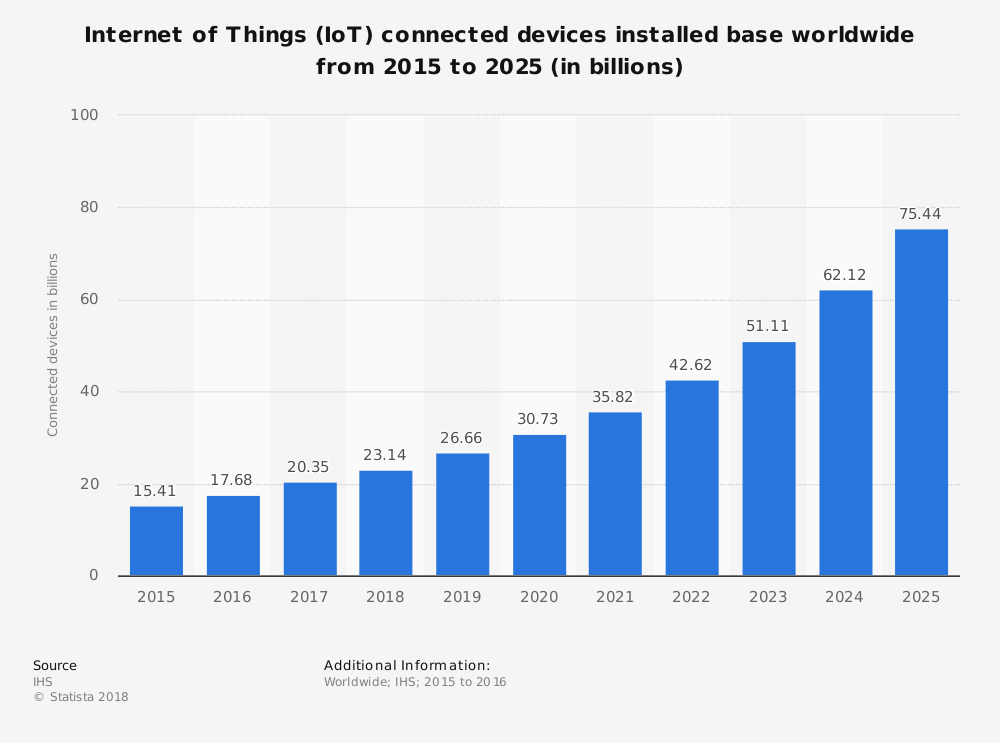
\includegraphics[width=150mm, scale=1]{Images/statista_iot.png}
      \caption{Statista: Predicted Growth in Online IoT Devices by 2025}
      \medskip
	  \small
		This graph is provided based on research by Statista Gmbh, showing their predicted growth trend for the number of internet-connected IoT devices by 2025. Historical data is included back to 2015.  
\label{fig:StatistaIoTPrediction}
\end{figure}

According to statistics published by Statista\footnote{Statista cite the original source of this data as being from IHS Markit, an analytics firm headquartered in London.} in 2018, \cite{StatisticIoTStatistics} by 2025 it is predicted that there will be over 75 billion IoT devices online globally: Several times greater than the human population of the world\footnote{The latest population statistics published by the Department of Economic and Social Affairs Population Division of the United Nations in 2017 \cite{UNWorldPopulation} estimate the population of the world at approximately 7.6 billion individuals.}\interfootnotelinepenalty=10000. Figure \ref{fig:StatistaIoTPrediction} shows their predicted exponential growth trend over the period from 2015. These devices include everything from environmental sensors to wearable technologies and process automation components, and are playing an increasingly important role in the lives of all members of society.  For a single IoT system, sensors could be used to collect information about a particular environment in a Wireless Sensor Network (WSN) configuration whilst communicating the information to a remote application, where it is aggregated and pushed to a set of distributed smartphones.


	
 \subsubsection{Security of IoT Devices}
Whilst connectivity between devices and processes has enhanced and optimised industrial processes, enabling the conception of countless new applications, the pace of this transformation has resulted in little to no attention being given to the security of these systems. Apart from concerns about the extent of pervasive monitoring conducted by IoT systems\footnote{The extent to which connected devices have become part of everyday life concerns many individuals, particularly since the primary purpose of IoT devices is to continuously gather, analyse and transport data to other systems. In an eye-opening paper published in 2017, \cite{7948540} Lackorzynski \textit{et al.} emphasise the dangers of internet-connected devices such as the \textit{Hello Barbie} childrens toy, which is ''a doll that could talk back to the user... in this case very probably a minor''. }, new applications are being found for IoT devices at such pace that instead of being built into these applications from the beginning, security is largely being left behind to catch up on later. Most of the time, it can be taken that there is no such thing as ''security by default''.

The risks - both to security and privacy - associated with the pervasiveness of the Internet in everyday life today are something that the general population are largely oblivious to. Insecam, which is a website broadcasting online feeds from thousands of IP cameras with default login credentials without the owners' knowledge, illustrates the gravity of this issue. \cite{Insecam} Devices and systems which never had communication capabilities before are being brought online, exposing them to significant potential tampering and misuse in ways that could affect the welfare of entire populations. Crucial systems on which society relies on a daily basis such as power grids, medical devices and traffic control systems are increasingly falling into this category, becoming exposed to attacks in a way that they never were in the past. 

Some of the greatest issues with the security of these devices include the following:

\begin{enumerate} \label{ReasonsForInsecureIoTDevices}
\item \textbf{Weak Default Credentials}

The main contributor to the success of most attacks on IoT devices  to date is the fact that these devices are shipped with weak default credentials that are identical across all instances of a given model. Additionally, these credentials are usually the only security measure used to mitigate against threats to these devices: There is very little effort required for an attacker to successfully compromise such a device.

\item \textbf{Limitations in Applying Updates}

The environments in which many IoT devices are deployed make it very difficult to patch vulnerabilities and apply updates to these devices. In general, large numbers of heterogeneous devices are deployed in a geographically dispersed, distributed setup and communicate over a variety of different networking protocols. Applying updates in such a deployment is inherently challenging.

\item \textbf{Limited Capacity for Encryption}

Due to the limited computational capacity and bandwidth of many low-powered IoT devices, the deployment of encryption on these devices is near to impossible. The compute-intensive operations required by most encryption protocols to both encrypt and decrypt data-in-transit and data-at-rest make it very difficult to implement encryption practically. To illustrate this, the Internet Engineering Task Force (IETF) stated in their most recent specification for Low-Powered Wide-Area Networks (LPWANs) that implementing key authentication mechanisms becomes ''challenging to handle in LPWANs with bounded bandwidth.'' \cite{ietf-lpwan-overview-10} As discussed by Dowling \textit{et al.}, if encryption is not implemented correctly, this can open the door for attacks on confidentiality, origin authentication and data integrity if the device in question is compromised. \cite{Dowling2017}

\item \textbf{Insecure Communication Protocols}

Many IoT devices use insecure communication protocols because of their requirement for low power consumption. The \textit{telnet} network protocol, which runs on port 23/TCP, has been largely retired as it is highly insecure, transmitting all traffic in clear-text including login credentials\footnote{The full telnet  protocol specification was finalised by the IETF 35 years ago in 1983, and explains the motivations behind the protocol and its intended uses. \cite{rfc854}}. It is however a lightweight protocol to deploy on a low-powered device, meaning that it has been widely included in IoT devices for authentication. This further weakens the security of these devices: A passive attacker eavesdropping on network traffic can capture IoT device data for later analysis or compromise the device itself.

\end{enumerate}

For attackers, IoT devices are very enticing: They are always online, using weak security mechanisms and often with access to powerful shells. The emergence of freely-available online scanning tools such as Shodan\footnote{Shodan is a search engine for internet-connected devices. If a search is performed for ''default password'', devices using default passwords are identified all over the world and returned to the user as a result. \cite{ShodanDefaultPasswordSearch}} mean that identifying these devices becomes trivial. As affirmed by leading cybersecurity expert Bruce Schneier in his article \textit{The Internet of Things is Wildly Insecure - And Often Unpatchable} in 2014, ''if we don't solve this soon, we're in for a security disaster as hackers figure out that it's easier to hack routers than computers''. \cite{TheresNoGoodWayToPatchTheIoT}

%% QUOTE SCHNEIER
\subsubsection{Internet of Things Botnets} \label{IoTBotnetsSoA}

Given the exponential growth in the number of internet-connected devices over the past several years, and given that attacks will always evolve as new technologies emerge,  new attack vectors and threats have been realised in relation to IoT devices since Bruce Schneier's insightful and telling article in 2014. \cite{TheresNoGoodWayToPatchTheIoT} Though many IoT devices are low-power devices commonly deployed in remote areas with low network bandwidth, large numbers of these devices can have a combined impact that packs a significant punch: Enter IoT botnets.

IoT botnets are likely the most active and topical breed of botnet at present. They are botnets composed entirely of compromised IoT devices. Most of these devices have been found to run the Secure SHell\footnote{The SSH protocol runs on port 22/TCP, and was designed by the IETF for secure remote login using encryption. \cite{rfc4252}} (SSH) and telnet authentication protocols with simple default username-password combinations, making it straight-forward to launch brute-force authentication attacks to gain root access to the device.

The highest profile attack to-date by an IoT botnet took the world by surprise in late 2016. The Mirai botnet, which amassed an army of over 300,000 IoT devices by capitalising on their poorly-implemented authentication mechanisms, conducted one of the biggest ever DDoS attacks by volume. The attacks began by targeting \textit{Krebs on Security}, \cite{KrebsOnSecurity} the website of well-known investigative security journalist Brian Krebs, eventually peaking at almost 1Tbps with an attack on French cloud hosting provider OVH. Research conducted by Antonakakis \textit{et al.} \cite{UnderstandingTheMiraiBotnet} on the success of Mirai found that for the 3 most common architectures found to be running the telnet protocol\footnote{MIPS 32-bit, ARM 32-bit, and x86 32-bit were the three most common CPU architectures identified in the collected device samples, accounting for circa 74\% of these. \cite{UnderstandingTheMiraiBotnet}}, ''security cameras, DVRs, and consumer routers represent(ed) the majority'' of these devices.

%\includewidefigure{UnderstandingTheMiraiBotnet_DefaultPasswordsTable}{The Mirai Botnet: Most Common Default Passwords}{A table provided in the \textit{Understanding the Mirai Botnet} paper, \cite{UnderstandingTheMiraiBotnet} showing the passwords that were most commonly found across all of the devices analysed in their research. }{Images/Understanding_the_Mirai_Botnet_-_table_of_default_passwords.png}

\begin{figure}[ht]
      \centering
      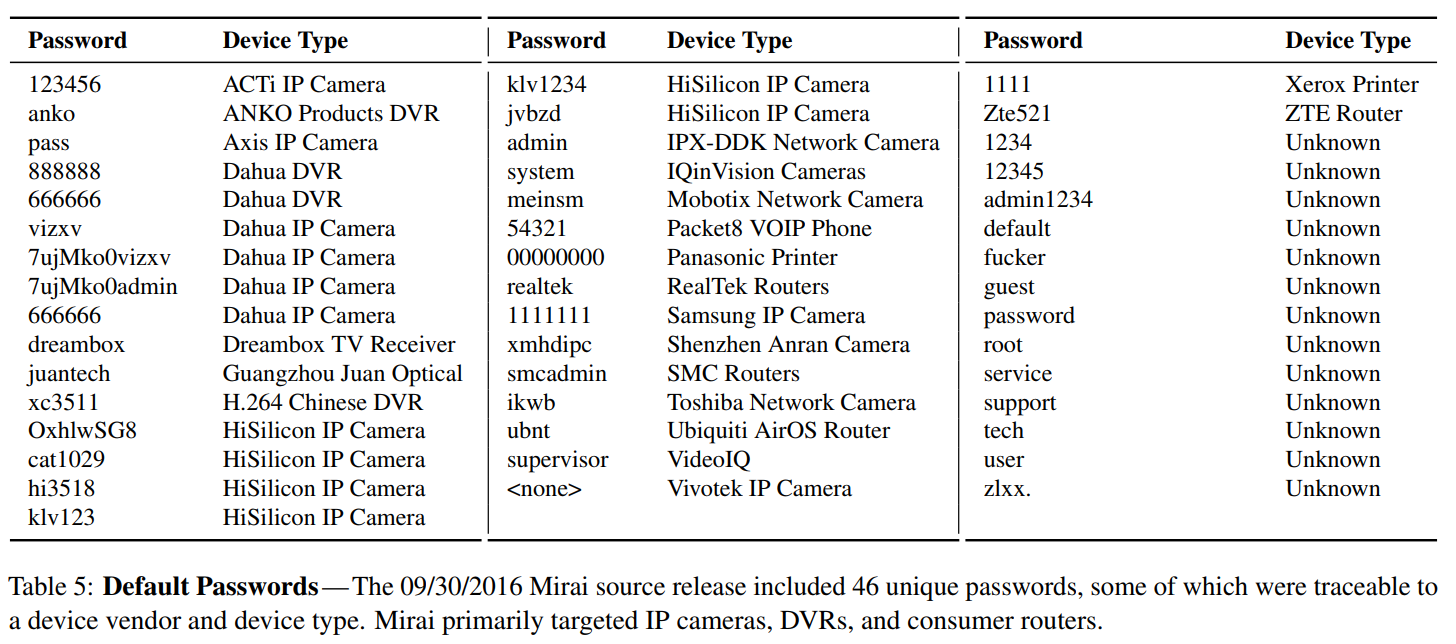
\includegraphics[width=175mm, scale=1]{Images/Understanding_the_Mirai_Botnet_-_table_of_default_passwords.png}
      \caption{The Mirai Botnet: Most Common Default Passwords}
      \medskip
	  \small
		A table provided in the \textit{Understanding the Mirai Botnet} paper, \cite{UnderstandingTheMiraiBotnet} showing the passwords that were most commonly found across all of the devices analysed in their research. 
\label{fig:UnderstandingTheMiraiBotnet_DefaultPasswordsTable}
\end{figure}

The scale and impact of this botnet was a revolutionary development. The fact that it was capable of threatening some of the worlds best-defended targets using enormous numbers of devices with low computational capabilities speaks volumes about the scale of issues that are currently being faced in IoT device security. As stated by Bruce Schneier in his 2017 article \textit{Botnet of Things}, ''botnets will get larger and more powerful simply because the number of vulnerable devices will go up by orders of magnitude over the next few years ... overall, the trends favor the attacker''. \cite{SchneierBotnetOfThings}

A number of other IoT botnets have surfaced since the Mirai attack, many of them variants of the original Mirai source code which was published online by a user called \textit{Anna Senpai} on the popular \textit{HackForums} site. \cite{WhoIsAnnaSenpaiKrebs} One noteworthy botnet is BrickerBot, an IoT botnet which surfaced shortly after the initial Mirai attacks on \textit{KrebsOnSecurity}. \cite{BrickerBotArticle} The author of this botnet, who calls themselves the \textit{janit0r}, claims to be a \textit{white hat}\footnote{This is a term commonly given to individuals who try to identify security vulnerabilities through hacking. They are different to malicious attackers in that they respect any relevant laws, and do not hack in order to damage the target system. Clearly, the \textit{janit0r} doesn't fit this description.} hacktivist intent on performing what they termed ''Internet Chemotherapy'': The complete destruction of IoT devices with poorly-implemented security measures as a punishment to their owners. In a farewell email made available to security site \textit{BleepingComputer} on 10th December 2017, the \textit{janit0r} warns that the world should ''WAKE UP TO THE FACT THAT THE INTERNET IS ONLY ONE OR TWO SERIOUS IOT EXPLOITS AWAY FROM BEING SEVERELY DISRUPTED'', and that organisations and individuals must take action to prevent this. \cite{janit0rFarewellEmail}


	
\subsection{Critical Service Infrastructures}
	
At a time where heightened political tensions exist between many of the world's most powerful nation states\footnote{The United States are currently locked in a cyber-combat against ''HIDDEN COBRA'', a codename for what they claim is North Korea's DDoS botnet infrastructure, as part of ongoing disputes between the two nations. A US national alert \cite{HiddenCobra} issued in June 2017 by the US-CERT claimed that HIDDEN COBRA had ''likely targeted the aerospace, telecommunications, and finance industries'' in the United States.}, cyber attacks are playing a prominent role in warfare and terrorism. Cyber attacks on critical service infrastructures have the potential to cause responses with severe impact.  Illustrating the severity of threats from competing nation states,  Unal \textit{et al.} \cite{NuclearReport2018} discuss the growing reliance of nuclear weaponry on digital technology and communication systems, stating that ''the likelihood of attempted cyber attacks on nuclear weapons systems is ... increasing from advanced persistent threats from states and non-state groups''.

In a report published in 2017 containing recommendations to the U.S. administration on national cyber-security, \cite{brenner_2017} M.I.T. researcher Joel Brenner states that one of the eight major challenges facing the United States government currently is to ''enable critical infrastructure operators to quickly identify and respond to cyber risk arising from cross-sector linkages as well as from their own network''. This statement encapsulates precisely the issues facing critical service providers worldwide today, and is something that is being reflected in incidents across the world with an increasing number of attacks on high-profile targets.

\subsubsection{Vulnerable Critical Infrastructures}
 It is clearer now than ever that key organisations and critical services require a renewed focus on defence strategies for their IT infrastructures. One such category of critical infrastructures is Supervisory Control and Data Acquisition (SCADA) systems, which are employed in industrial control environments to perform functions such as process control and monitoring. Typically, these systems deal with lots of components including sensors and mechanical parts like motors, enhancing the efficiency of operations in these environments. 
 
 Securing these systems is vitally important: They are the underlying control system of almost all nation-critical infrastructures such as transport, power and water. It is clear that the consequences of compromising these systems have the potential to be serious and far-reaching.

\subsubsection{Case Study: National Health Service Attacks 2017} \label{WannaCryNHSCase}
In May 2017, one of the more memorable attacks in recent years on a nation-critical service occurred in the United Kingdom. The global WannaCry \textit{ransomware} attacks, which successfully compromised more than 200,000 systems in over 100 countries, knocked systems in the UK National Health Service (NHS) at 37 sites offline for over a week with more than 6,912 appointments cancelled in that time. Though the NHS was almost certainly not a specific target of the ransomware authors\footnote{According to a paper published in the aftermath of the attacks, many other sectors across the world including transport and energy were also affected. \cite{MakingSenseOfRansomwareMess}}, the attacks had a huge impact on health services across the UK. \cite{AmyasMorseWannacry}

%\includewidefigure{NHS_WannaCry_Illustration}{Illustration of WannaCry Infection in the NHS}{An illustration of the infection of systems at NHS hospital sites by the WannaCry ransomware. The infection was not limited to user devices and servers, affecting systems including MRI scanners and blood test analysis devices. \cite{LessonsLearnedWannacryReport}}{Images/NHS_WannaCry.png}

\begin{figure}[ht]
      \centering
      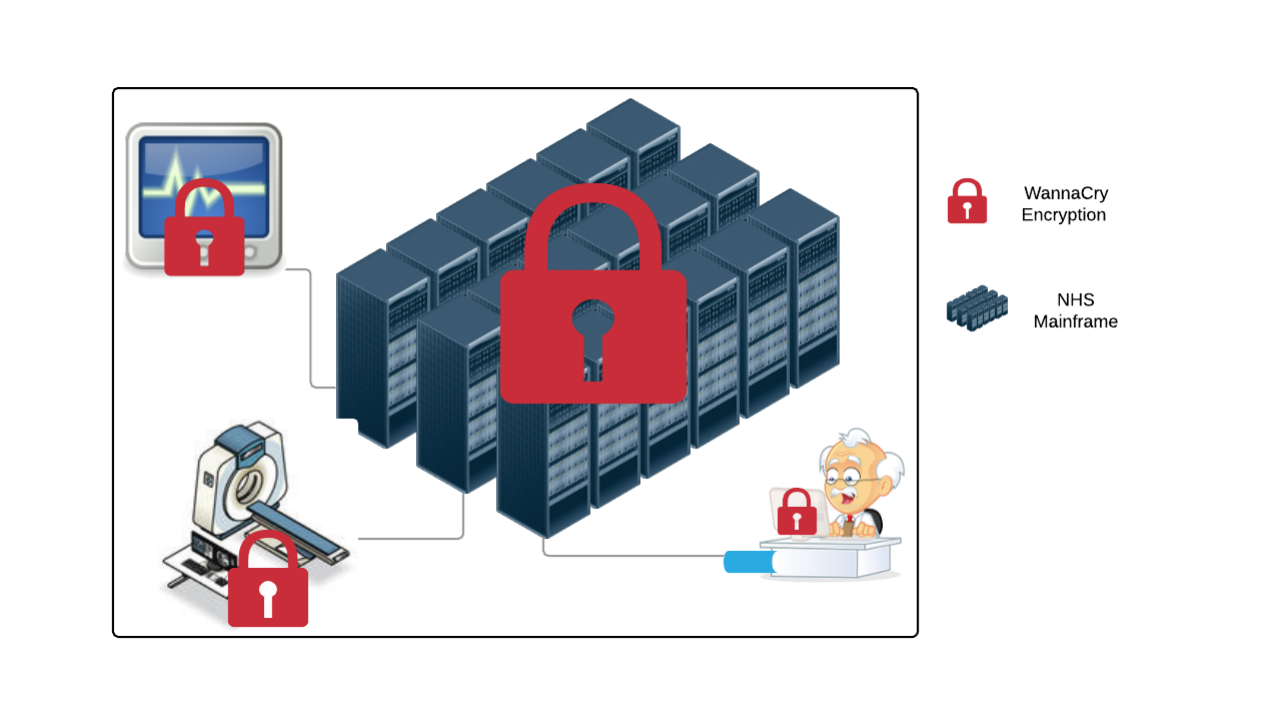
\includegraphics[width=150mm, scale=1]{Images/NHS_WannaCry.png}
      \caption{Illustration of WannaCry Infection in the NHS}
      \medskip
	  \small
		An illustration of the infection of systems at NHS hospital sites by the WannaCry ransomware. The infection was not limited to user devices and servers, affecting systems including MRI scanners and blood test analysis devices. \cite{LessonsLearnedWannacryReport}
\label{fig:NHS_WannaCry_Illustration}
\end{figure}

Examining the compromise of the NHS infrastructure by the WannaCry ransomware presents a strong basis for addressing many issues seen across critical service infrastructures. Being such a high-impact incident, it emphasises the severe consequences that a cyber attack can have on a critical service. An audit report published by the UK National Audit Office after the incident \cite{AmyasMorseWannacry} highlights a number of substantial shortcomings in the NHS security defence strategies up to 12th May 2017 when the attacks occurred:
	
	\begin{enumerate}
		
		\item There was no incident monitoring in place to alert security first-responders to any unusual behaviour in the NHS systems: Evident from the fact that it took over half a day to reach those who could take remedial action. 
		
		\item There was no centralisation of system data, meaning that security experts had to physically attend the affected sites in order to collect crucial data about the attacks. This further prolonged the period for which these systems remained inoperable. 
	
		\item Prior to the incident, recommendations regarding  updates for the NHS IT systems were issued but not followed at the affected sites. Further to this, there was no system in place to determine whether or not the actions had ever been taken. Outdated and unpatched operating systems were a major contributor to the success of the compromise, which was entirely based on a Windows exploit\footnote{WannaCry and NotPetya, two ransomware strains which made their first appearance in 2017, both exploited this vulnerability. Officially named 'EternalBlue MS17-010' by Microsoft, a patch was released for it after major attacks by both of these ransomware strains. According to an article by Brian Krebs, \cite{KrebsWannaCry} The EternalBlue vulnerability exploits the Microsoft Server Message Block (SMB) network file sharing protocol. SMB allows applications on a computer to read and write to files and to request services that are on the same network.}.	
	\end{enumerate}
	
	% How did it happen exactly? A trusted node on the outskirts of the network (such as a GP) received the infection, and it was propagated back into the NHS mainframe where is was able to root itself and spread to other parts of the network.
    
    Ultimately, the lack of monitoring within the NHS systems meant that when the attacks occurred, the systems at the affected sites remained offline for an extended period of time, causing chaos across the entire healthcare system in the UK.  It is clear that in order to protect both their own systems and those of others that depend on them, organisations must place emphasis on security training for their members, the security and maintenance of their technologies, and the rigorousness of governance of their systems. 




%%
%%	Section 2: Intrusion Detection Technologies
%%
%%


\section{Intrusion Detection} \label{IntrusionDetectionSection}

An Intrusion Detection System (IDS) is a security application that is employed to detect attempts from an attacker to gain unauthorised access to a system or system resource. They are usually deployed in a region known as the De-Militarised Zone (DMZ), a sub-network separating an internal network from untrusted external networks, providing an added layer of isolation between internal and external systems\footnote{Usually, content-serving systems are placed in this region of the network so that they can be accessed from external networks.}. Most traditional IDSs work off the basis of comparing activities to a defined security policy, and either permitting or denying the action on this basis.

In this section, the motivations for intrusion detection, along with two primary types of intrusion detection system, are discussed and compared.


\subsection{Motivations for Intrusion Detection} \label{MotivationsForIntrusionDetection}
IDSs play an important role in securing both enterprise and personal systems. Among the many advantages are the following:
\begin{itemize}
\item By detecting an intrusion in the early stages, the intruder can be removed from the system before any damage is done.
\item Attackers in general strive to remain anonymous and undetected. If a potential intruder has some knowledge of an effective IDS being in place in a system, they may be deterred from proceeding with an attack.
\item Valuable information may be collected about the nature of the intrusions and how they took place, enabling administrators to continuously re-evaluate their system design and security strategies. 
\end{itemize}

How each of these advantages are provided, and to what extent, is dependent on the type of IDS being employed. It should be recognised that threats can come from nodes both internal and external to the network in question, and so a maximally effective IDS will address both. 

IDSs can be broadly categorised as either being \textit{passive} or \textit{active}.
\begin{itemize}
\item Passive IDSs are not proactive about preventing or interfering with attacker activities.
\item Active IDSs are proactive about engaging with the attacker in order to counter an attack.
\end{itemize}


In this section, two particular IDSs will be discussed in detail: firewalls and honeypots.


\subsection{Firewalls}

Firewalls are the most commonly deployed type of IDS, and are used in virtually all enterprise networks as part of an organisation's network security. In general, they are classified as a \textit{passive network defence mechanism}. According to a literature survey by Voronkov \textit{et al.}, "a firewall is a system consisting of software and/or hardware that is designed to prevent unauthorized access to/from a network or device". \cite{Voronkov:2017:SLR:3161158.3130876}



\subsubsection{Overview}
The basic principle of operation of a firewall is to act as a barrier on the periphery of a network, preventing intruders and malicious forces from gaining access  to the system being protected. In practical terms, they filter network packets based on a defined security policy which is a set of configured rules, and either accept or reject a given packet according to this policy.


%\includewidefigure{Firewall_DMZ_Illustration}{Use of Firewalls in a De-Militarised Zone}{An illustration of a typical corporation network where firewalls have been employed at the internal and external entrypoints to the De-Militarised Zone (DMZ).}{Images/Illustration_of_Firewalls_in_a_DMZ.png}

\begin{figure}[ht]
      \centering
      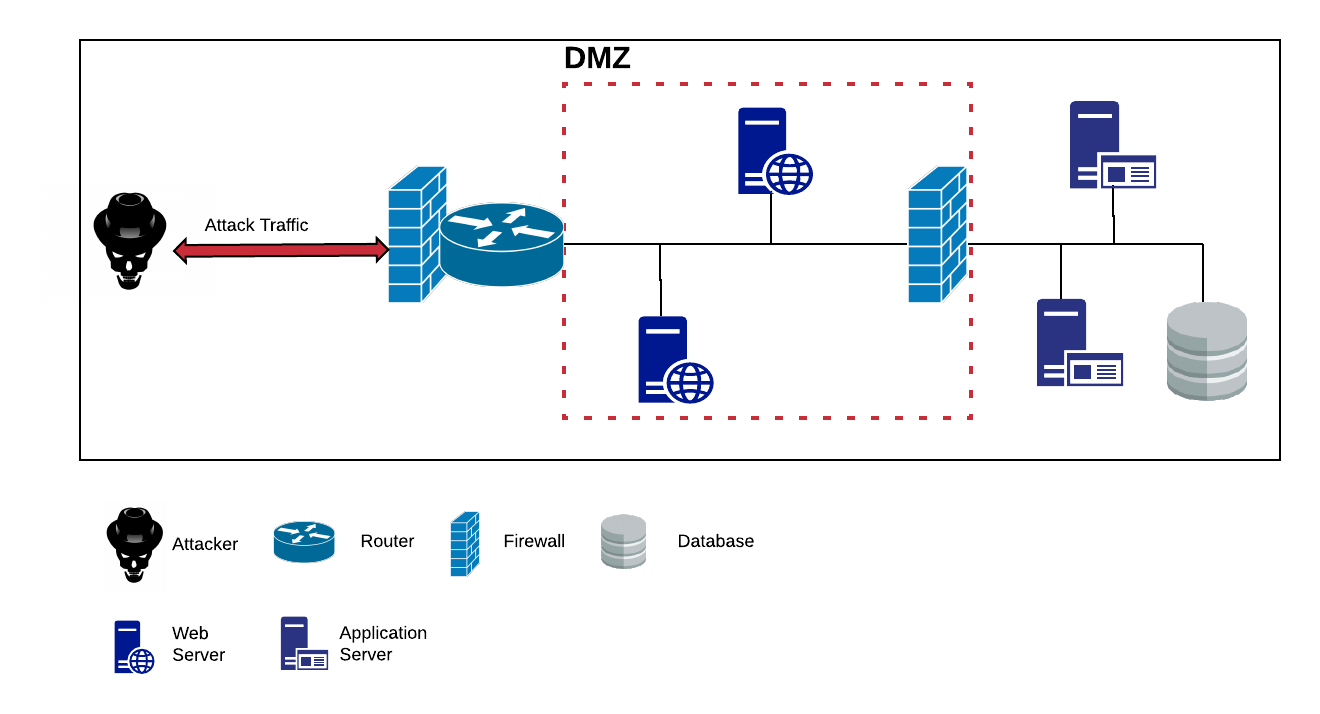
\includegraphics[width=175mm, scale=1]{Images/Illustration_of_Firewalls_in_a_DMZ.png}
      \caption{Use of Firewalls in a De-Militarised Zone}
      \medskip
	  \small
		An illustration of a typical corporation network where firewalls have been employed at the internal and external entrypoints to the De-Militarised Zone (DMZ).
\label{fig:Firewall_DMZ_Illustration}
\end{figure}

\subsubsection{Design}
A number of commonly employed approaches to implementing firewall policies are identified by Omar Santos in \textit{End-to-End Network Security defence-in-Depth}. \cite{OmarSantos} Some of these are described as follows:

\begin{itemize}
\item \textbf{Pattern Matching}

The firewall tool searches for a fixed sequence of bytes within a packet, often aligned at a specific position corresponding to a field within the packet. It then makes a filtering decision by consulting its defined security policy.

One of the primary limitations of pattern matching is that it generally exhibits a high rate of false positives, making it relatively inaccurate as a technique of classifying packets that should be denied access. 
\item \textbf{Protocol Analysis}

Protocol analysis is accomplished by decoding protocol-specific communications, i.e. by examining the packets corresponding to particular communication protocols. The firewall will identify elements of the protocol and examine them for an infringement, for instance by examining explicit fields within the packets. An example for an SMTP packet might be examination of fields such as \textit{HELO}, \textit{MAIL}, \textit{RCPT}, \textit{DATA}, \textit{SET}, \textit{NOOP}, and \textit{QUIT}.
\item \textbf{Heuristic-Based Analysis}

Also known as \textit{misuse detection}, this technique tries to identify intruders based on a set of known undesirable behaviours and patterns that can be determined according to rules. Systems built upon this concept are severely limited in intrusion detection capabilities since they cannot detect an intrusion for which no rule is defined. 

\item \textbf{Anomaly-Based Analysis}

Anomaly-based analysis techniques try to define the behaviour of a normal user over time, and compare the behaviour of all users to this in order to identify suspicious behaviour that may relate to an intrusion. 

\item \textbf{Deep-Packet Inspection}
 
Deep-Packet Inspection (DPI) involves closely examining information embedded in network packets in order to make more informed decisions about how to handle the packet. This often allows for more effective mitigation against attacks such as DDoS, where DPI allows for the more accurate identification of packets that have undesirable contents or are in some way not legitimate.

\end{itemize}


\subsubsection{Challenges} \label{ChallengesForFirewalls}

% 

% Passive security mechanisms in general are notoriously hard to deploy, e.g. IPSEC, DNSSEC, etc. Firewalls are no different: They are very restrictive for the normal use and operation of the system they are deployed in, and so are often configured incorrectly or ineffectively in order to facilitate usability.

There are a number of issues with using firewalls alone for intrusion detection. Though at a point in time these systems reflected the configuration of enterprise networks accurately, in the world of the modern web many of the premises of using firewalls simply do not hold any more. As enumerated by Steven M. Bellovin in \textit{Thinking Security: Stopping Next Year's Hackers}, \cite{ThinkingSecurityBellovin} the design and use of firewalls is based on the following premises:


\begin{enumerate}
\item A firewall operates at a \textit{topological chokepoint} in the network it is protecting, such that it partitions two sections of the network.
\item All nodes being protected inside the firewall have the same security policy.
\item All nodes inside the firewall are trusted.
\end{enumerate}

If all of these conditions hold, then a firewall will work well in the system in question. However, taking any modern IT infrastructure in an organisation today, most - if any - of these assumptions do not hold true. 
\begin{itemize}
\item Enterprise networks increasingly deal with nomadic users, who are facilitated in constantly connecting to and disconnecting from these networks without any security auditing being performed.
\item The devices that connect to enterprise networks today are incredibly diverse, and implement an even more diverse and inconsistent range of security policies.  
\end{itemize}

On top of this, it is increasingly becoming difficult for firewalls to use packet inspection techniques to filter network traffic because of incompatibility with other security mechanisms. An increased uptake in TLS encryption and the push for packet header encryption is causing enormous issues for the operation of firewalls, which cannot decrypt packets in order to make the required filtering decisions that it depends on.

There is no question that firewalls are no longer sufficient on their own in providing security for modern networks. They can be reasonably effective against known, less sophisticated attacks and are less effective against more sophisticated targeted attacks which are more likely to use new exploits. As Fred Schneider explains in his paper \textit{Blueprint for a Science of Cybersecurity}, ''a secure system must defend against all possible attacks - including those unknown to the defender. But defenders, having limited resources, typically develop defences only for attacks they know about.'' \cite{Schneider11_BlueprintForScienceOfCybersecurity}

Overall, firewalls are most effective when used in combination with other security mechanisms, but their inability to classify and mitigate against new threats is a major limitation to their use. \cite{ThinkingSecurityBellovin}

%% Could also talk  about the limitations of using firewalls, since it is far more likely that a legitimate user will be identified as an intruder: Pessimistic assumption that the user is more likely to be an attacker than a harmless user.


\subsection{Honeypots} \label{HoneypotsSection}

%% Deception is the primary underlying principle behind the use and design of honeypots: They serve as a deterrent, since an attacker may waste valuable time pursuing misleading information instead of achieving their goals.


Well-known security expert and Honeynet Project founder Lance Spitzner defines honeypots as "a security resource who's value lies in being probed, attacked or compromised". Honeypots leverage the concept of deception in order to combat attackers. As explained in a paper by Cliff \textit{et al.}, ''the essential parts in cyber deception include crafted information by the defender (that will be used to mislead) and wrong actions taken by the adversary as a result of the deception.'' \cite{8328971}

Put simply, honeypots are devices which masquerade as legitimate and systems in order to detect, track and analyse patterns of user behaviour when the system is illegally accessed. They are categorised as an \textit{active network defence mechanism}, and are deployed solely with the intention that they will be attacked.  A key characteristic of a successful honeypot is attractiveness to an attacker. 'Attractive' in this context means that the honeypot should appear to be exactly the device that the attacker is looking for: A device that has the potential to be easily exploited, whilst offering maximum value to the attacker. 

%% Honeypots try to make it more difficult for an attacker to gain anything from attacking a network.
%% Honeypots work off the principle of deception.

\subsubsection{Overview}

Honeypots are broadly seen as acting as both decoys and sensors in the network in which they are deployed.

\begin{itemize}
\item \textbf{Honeypots as Decoys}

A honeypot can be used to divert an attacker's attention away from the valuable components of the network in which it is deployed. This is particularly useful in a production environment, when there is a need to protect important systems on the network. 

In order for this strategy to be effective, the honeypot should appear to be exactly what the attacker is looking for. By then being attacked, the honeypot can immediately notify system administrators of an intruder being present in the network, allowing them to take the appropriate course of action to secure it.

\item \textbf{Honeypots as Sensors}

Honeypots can also be viewed as sensors, since they can collect valuable data about the attacks that they receive. This is particularly useful for detecting weaknesses and vulnerabilities in system design, since the captured attack data can be analysed to understand the attacker's behaviour and strategies as well as their motivations.
\end{itemize}

Thus, the value of honeypots is both in their ability to capture information as well as to defend the system within which they are deployed.

Amongst the many benefits of using honeypot technologies are the following:

\begin{enumerate}
\item \textbf{Configurability}

In general, honeypots are highly configurable and customisable and can be made to mimic real systems. This configurability allows those deploying them to adapt their defence strategy to tackle evolving attack behaviours.

\item \textbf{Inside the Network} 

Honeypots are deployed inside the infrastructure of the system they are protecting, rather than on the fringes as with firewalls. This allows for security much closer to the real systems that are being targeted by attackers.

\item  \textbf{Logging Capabilities} 

Honeypots give a unique opportunity to capture valuable information about the nature of attacks being launched against a system, providing a means of observing attackers 'in the wild' without being detected. This gives system administrators a better chance of staying up-to-date with the evolving security requirements of their systems.

\item  \textbf{Few False Positives}

The premise of using a honeypot is that nobody should communicate with it: There is no legitimate reason to interact with a honeypot, since it is deployed with the sole purpose of attracting attacks. This means that typically, a honeypot will trigger very few false positives, since every interaction with a honeypot is automatically distrusted. This has added benefits for system administrators in that there is a lesser requirement to comb through very large log files in order to identify a significant event, which is common practice with firewalls and many other IDSs.

It is important to consider however that individuals within an organisation may mistakenly interact with the honeypot out of curiosity, something which can often be deduced from looking at the logging captured. In general, the presence of honeypots in a system should not be well-known within the organisation for this reason.

\item  \textbf{Offensive and Defensive}

As explained, honeypots are an active defence mechanism. They allow for learning about adversarial intent, capability, and techniques as well as thwarting attempts to compromise real systems. By using honeypots, cyber attacks can be mitigated against by making access to valuable systems both expensive and ineffective.
\end{enumerate}


\subsubsection{Design} \label{HoneypotDesignSoA}
The design of honeypots to suit the context of their deployment is key to their ability to provide effective intrusion detection in a system. The primary design categorisations of honeypots were outlined in a paper by Mokube \textit{et al.} \cite{Mokube:2007:HCA:1233341.1233399} on the basis of (i) their level of interactivity with an attacker, and (ii) the context of their deployment.

\paragraph{Interactivity} \label{HoneypotInteractivityLevels} \mbox{}\\ 
Interactivity levels of honeypots are an important consideration, which define (i) the ability of the attacker to interact with the honeypot, and consequently (ii) the volume and type of information that can be gathered by that honeypot. Levels of interaction range from simply allowing a connection to be made, to being able to download and install malware binaries. The cost versus learning benefits of honeypot interactivity levels increase proportionally, meaning that a highly interactive honeypot will likely be expensive to host and maintain. 

Any effective honeypot must be capable of interacting at some level with an attacker, while also quietly monitoring their actions. There are three practical classifications of honeypot interactivity level: Low, high and medium.

\begin{itemize}
	\item \textbf{Low}
	
	Low-interaction honeypots are most commonly used to alert someone to the fact that an attack has occurred, but do not provide any means of interacting with the attacker or capturing the attack data. They are used in cases where a lower-risk solution is preferred: In general, a low-interaction honeypot will simply be an emulation of a real service, and so does not offer any opportunity for system compromise by an attacker. This can be a major limitation to their use, since there is very little knowledge to be gained from preventing further interaction with an attacker.
	
	\item \textbf{High}
	
	High-interaction honeypots are at the other end of the spectrum compared to low interaction honeypots. They are fully-fledged systems, and give the opportunity for attackers to use real applications during their interactions. A great deal can be learned about the nature of attacks from using high-interaction honeypots, since it is the closest thing to observing attacks ''in the wild''. The trade-off is the high-risk associated with the exposure of a real device to a malicious attacker, which in the worst case could see the entire system taken over by an attacker and used to launch further attacks on other devices. Some of the ethical considerations around this issue are discussed in \textit{Section \ref{EthicsOfHoneypots}.}
	
	\item \textbf{Medium}
	
	As described, the appropriate level of interactivity of a honeypot depends on the use context: Low-interaction devices are commonly used for detecting connection attempts, whereas high-interaction devices are live systems that can capture detailed information about the behaviour of attackers ''in the wild''. Medium interaction honeypots offer a good middle-ground, using emulated components of a real system to allow a level of interactivity with the attacker whilst not exposing any real systems that could be compromised.
	
\end{itemize}

A summary of the characteristics of each of these categories of honeypot are given in table~\ref{table:honeypot-interaction}.

\begin{table}[!h]
	\begin{center}
		\begin{tabular}{|c|c|c|c|} 
			\hline
			\bf Interaction Level  & \bf Information Quality  & \bf Risk  & \bf Maintenance Cost \\
			\hline
			High & Excellent & High & Difficult  \\
			Low & Poor & Low & Simple \\
			Medium & Good & Medium & Relatively Simple \\
			\hline
		\end{tabular}
	\end{center}
	\caption[Comparison of Interaction Levels of Honeypots.]{A summary of the characteristics of each different honeypot interactivity level, similar to that provided in a survey of honeypot technologies by Nawrocki \textit{et al.}. \cite{Nawrocki2016} In general, the higher the interaction level the higher the cost, risk and value of information captured.}	
	\label{table:honeypot-interaction}
\end{table}

\paragraph{Deployment Scenarios}

There are primarily two deployment scenarios for honeypots: Production and research. This distinction mainly distinguishes between the function that the honeypot needs to provide for the system in which it is to be deployed.

\begin{itemize}
	\item \textbf{Production Honeypots}
	
	Production honeypots are generally deployed in large, enterprise networks with the intention that they will act as a part of the active network defence in the organisation's infrastructure. An example of such a deployment is shown in figure~\ref{fig:Honeypot_DMZ_Illustration}. Their primary purpose is to act as a decoy, luring the attacker away from valuable machines on the network with a seemingly more valuable and vulnerable target. This enables the honeypot to alert system administrators early on to the fact that there has been an intrusion, giving them the opportunity to isolate the valuable devices in the network from the infected honeypot. As previously highlighted, it also enables system administrators to identify vulnerable points in their infrastructure.


%\includewidefigure{Honeypot_DMZ_Illustration}{Use of Honeypots in a De-Militarised Zone}{An illustration of a typical corporation network where honeypots have been employed in conjunction with internal and external firewalls, inside the DMZ.}{Images/Illustration_of_Honeypots_with_Firewalls_in_a_DMZ.png}

\begin{figure}[ht]
      \centering
      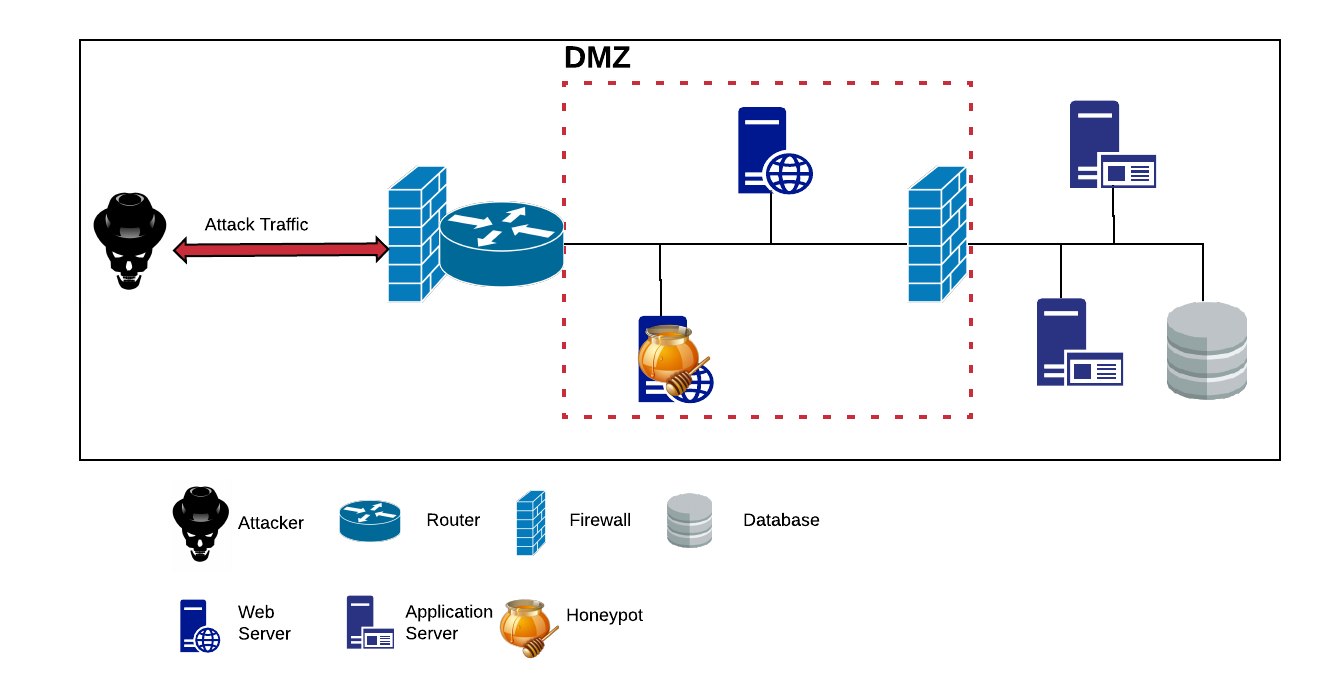
\includegraphics[width=160mm, scale=1]{Images/Illustration_of_Honeypots_with_Firewalls_in_a_DMZ.png}
      \caption{Use of Honeypots in a De-Militarised Zone}
      \medskip
	  \small
		An illustration of a typical corporation network where honeypots have been employed in conjunction with internal and external firewalls, inside the DMZ.
\label{fig:Honeypot_DMZ_Illustration}
\end{figure}
    
	The idea of attracting attackers into the system, encouraging them to interact with it and give away their attack strategies without causing any harm to the systems with real production value is the major attraction of using honeypots in a production environment. 
	
	
	\item \textbf{Research Honeypots}
	
	As the name suggests, these honeypots are generally deployed for the purpose of research rather than as a security measure. The emphasis with these honeypots is not so much on the ability of the honeypot to act as a decoy, and more on the ability of the honeypot to collect valuable data for analysis. By allowing attackers to interact with and infect the honeypot, research can be carried out relating to the behaviour and strategies of the attackers.
	
\end{itemize}

\subsubsection{Comparison with Firewalls}

When compared to traditional, passive intrusion-detection mechanisms such as firewalls, honeypots exhibit some crucial differences. 

\begin{itemize}
\item Firewalls define all attackers passively and simply alert to the fact that a security incident, such as an unauthorised connection attempt, has occurred. A system administrator can then, for instance, blacklist\footnote{Blacklisting an IP address means that it is added to a list of addresses that aren't considered trustworthy.} the source IP address of the connection to deny it access to the system. 

However, if a new attack comes along for which there is no rule defined in the firewall's security policy, the firewall is not able to deal with this attack. This illustrates how firewalls can only provide \textit{known-threat mitigation}.
\item In contrast to firewalls, honeypots proactively entice attackers to give away their attack strategies and intentions by leaving their tracks behind on the device. This enables the same system administrator to do far more to enhance their system security policies and identify potential flaws in their infrastructure, allowing them to \textit{improve} their system's security. 

As well as this, the honeypot can attract and deal with previously \textit{unknown threats}, giving them another edge over firewalls since they can provide \textit{unknown-threat mitigation} as well as \textit{known-threat mitigation}.
\end{itemize}

By using honeypots, system administrators are able to learn what attackers are targeting in their systems, enabling more effective defences to be implemented as vulnerabilities and flaws are identified. As suggested by Bellovin, ''the world has changed ... the decision to rely on (firewalls) should be reexamined and perhaps abandoned''. Despite this, firewalls are not obsolete and will continue to play an important role in IT and network security with their ability to detect and classify potential security risks at the edge of the network they are protecting. They are however best used in conjunction with active network defence mechanisms such as honeypots. \cite{ThinkingSecurityBellovin}


\subsubsection{Honeynets} \label{HoneynetsExplanationSoA}
%% Describe honeynets and how they can be beneficial as part of the network security of a system.
Honeynets are networks of interconnected honeypots, which coordinate their efforts to provide active network defence. Given that they consist of more than one honeypot, they have additional abilities to capture valuable attack information regarding threats compared to standalone honeypots: For instance, it is possible to study the propagation of attacks from one honeypot to the next, and to simulate a variety of different systems that may attract different categories of attack.

Honeynets are significantly more complex than standalone honeypots given that they consist of a network of honeypot devices designed to be attacked. In general, a honeynet will contain \textit{high interaction} honeypots so that an attack is able to propagate from one real system to another real system. As with individual honeypots, any connections to a system in the honeynet are immediately distrusted and assumed to be malicious. 

An element of a honeynet which is described by Lance Spitzner in \textit{Honeypots: Catching the Insider Threat} \cite{Spitzner:2003:HCI:956415.956438} is something that he refers to as the \textit{honeywall gateway}, a bridging device between external systems and the honeynet. All traffic between the external system and the honeynet must pass through this gateway. The honeywall will typically have two interfaces: One to connect it to the external web, and the other to connect to the honeynet. The honeywall thus acts to separate the honeynet from the external web. Since the honeynet is only reachable through the honeywall, which can monitor and control network traffic to and from the honeypots in the network, extensive extra monitoring can be performed on attackers of the system. Depending on the configuration, this component has the opportunity to capture data including network traffic and keylogging data.

\begin{figure}[ht]
      \centering
      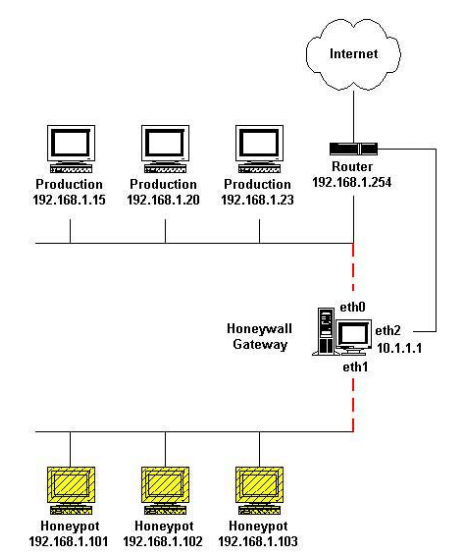
\includegraphics[width=100mm, scale=0.6]{Images/honey-wall-without-meta-data.png}
      \caption{Lance Spitzner's Proposed Honeynet Architecture}
      \medskip
	  \small
		This figure shows a diagram taken from Lance Spitzners paper proposing a honeynet architecture. Original source: \textit{Honeypots: Catching the Insider Threat}. \cite{Spitzner:2003:HCI:956415.956438}     
\end{figure}

% ^.
In summary, using a honeynet allows for deployment of a highly-controlled active defence network where all activities of attackers are made visible. The insights that can be gained from observing the behaviour of attackers in an unrestricted networked environment are highly valuable to those who wish to continuously improve their system defences. However, the risk associated with hosting a system of this type is a major trade-off since there are many more points of failure in a network of intentionally vulnerable devices.


%\subsubsection{Honeypots for Botnet Analysis}
%Honeypots have been widely used in the study of botnets and other categories of attacker.
%They provide researchers and reverse engineers with a platform to analyse both infection and operation of malware. Botnets are just a subset of this malware, where it is interesting and useful to study the operation of the malware as it is executing. High interaction honeypots thus seem to be a great solution for this problem.

\subsubsection{Challenges} \label{HoneypotSoAChallenges}
There are a number of challenges to the widespread deployment of honeypots in networks, outlined below.
	\begin{enumerate}
    
    \item {\textbf{Detection}}
    
	One of the major considerations when designing or using a honeypot-driven solution is the risk of the honeypot being detected as a non-genuine system. This is particularly relevant to low and medium-interaction honeypots which emulate a real system: It is never possible to exactly mimic the behaviour of the corresponding real system. This means that carefully crafted actions by an attacker may allow them to detect that they are not interacting with a bona-fide system by triggering different responses: A form of fingerprinting. It is an ongoing challenge for honeypot designers to combat fingerprinting checks by attackers.
    
    In general, honeynets are less likely to be fingerprinted successfully than an individual honeypot since they provide a network of interconnected high-interaction honeypots providing real services. This kind of system is highly enticing to attackers because of the advanced system capabilities that it provides, and thus a less likely suspect as a non-genuine system.

	\item{\textbf{Adoption}}
    
	There are many challenges to overcome in order to make the use of honeypots more widespread. To many, the idea of inviting a malicious actor into a production system seems like a potentially destructive action, and so many system administrators do not consider honeypots as part of their security infrastructure. Canary, a honeypot solution developed by Thinkst Applied Research, highlight on their product landing page the challenge behind adopting honeypots in large networks: ''With all the network problems we have, nobody needs one more machine to administer and worry about''. \cite{CanaryThinkst} Although it could be argued that this is a sales pitch, this statement highlights the demand and lack of supply of feasible solutions for large organisations regarding deployment and maintenance of honeypot-based systems. 
	
	\item{\textbf{Ethical Concerns}}
    
 	The use of any surveillance technology, which is the category into which honeypots fall, has ethical questions associated with it. Honeypots are widely accepted as an ethical approach to intrusion detection and understanding cyber attacks. Since there is no legitimate reason for interacting with a honeypot, any interactions are likely to be of a malicious nature - in which case, the honeypot simply serves to counteract further attacks of this type in the	future. Mokube \textit{et al.} discuss these ethical issues in detail in their paper. \cite{Mokube:2007:HCA:1233341.1233399} However, a discussion in a whitepaper published by the System Administration, Networking, and Security Institute (SANS), \cite{SANSPreemptiveDeterrence} it can be concluded that their use does not involve:
 	
 	\begin{itemize}

 		\item Entrapment, since there is no inducement to attack the honeypot - rather, it is something that all devices are vulnerable to because attackers will always seek to attack devices within their reach, regardless of whether it may be a honeypot. As aptly phrased by security researcher Lance Spitzner \cite{HoneypotsAreTheyIllegalSpitzner}, ''attackers find and break into honeypots on their own initiative''.
 	
 		\item Invasion of privacy, since surveillance mechanisms are broadly seen to be acceptable where they serve simply to protect their own environment. A commonly encountered example in physical environments is the use of CCTV cameras.
 		
	\end{itemize}

		Overall, the ethical concerns around the use of honeypots are widely accepted to be resolved by the nature of the deployment of honeypots: Ultimately, their purpose is to defend against unethical actions by attackers. With reference to the research being undertaken in this project, ethical considerations are discussed later in relation to the design of the research environment in \textit{Section \ref{EthicsOfHoneypots}}.
\end{enumerate}

\subsection{Cyber-Incident Monitoring}
Cyber-incident monitoring forms an important part of providing effective intrusion detection. Cyber incident monitors are platforms that support system administrators in identifying and acting upon threat intelligence collected through intrusion detection mechanisms such as honeypots and firewalls, primarily through providing enhanced usability and more effective communication. It is concerned with the effective management of intrusion detection tools, the recording of threat events, and the provision and presentation of threat information to first-responders. 

 %adding visual aids to the interpretation of honeypot data is a key element to bringing security into container-based architectures.

\subsubsection{Usability in Security}
It is widely accepted that the ability of a user to easily employ security systems makes a crucial contribution to their effectiveness: As argued by Sasse \textit{et al.}, ''security mechanisms are often too time consuming for people to bother with, or so complex that even those willing to use them make mistakes.'' \cite{7676149} The use of security mechanisms adds an overhead to the use of systems almost without exception. Apart from the consequent disincentive for individuals to use these mechanisms, it becomes very hard to use them effectively when their use is not straight-forward.

In a literature review addressing the usability of firewall applications in particular, Voronkov \textit{et al.} found that usability studies could greatly enhance the effectiveness of security mechanisms, since configuring them ''is a process that is complicated and prone to error...  misconfiguration of firewalls leads to a broad number of vulnerabilities in the network; environments with distributed and multiple firewalls just make matters worse.'' \cite{Voronkov:2017:SLR:3161158.3130876}

\subsubsection{Visualisation in Security}
Visualisation techniques have become crucially important in delivering usable security solutions. Security problems are inherently complex: In the case of tools such as firewalls which work off the basis of a list of defined rules, it becomes very difficult to understand and maintain the overall security policy as the list grows.

The impact of using visualisation in security mechanisms is that threat intelligence is communicated more clearly and effectively to those consuming the data. Ease of visibility of the state of a system is a crucial element of active network defence in identifying and investigating potentially malicious activities and detecting unknown threats before they can do damage. As explained by Vasilomanolakis \textit{et al.} in a paper detailing the development of a honeypot-based incident monitoring system, such a system ''unif(ies) the various alert generators into a single system that assists the user to make informed decisions''. \cite{Vasilomanolakis}



%%
%% 	SECTION 3: Modern System Infrastructures 
%%
\section{Modern System Infrastructures} \label{ModernSystemsInfrastructures}
There is a significant shift in the hosting solutions that are being used by large organisations that rely heavily on their IT infrastructure, particularly for those providing services on such a platform. Outsourcing of resource management is now the preferred approach for many large organisations, given that specialised hosting providers are increasingly offering end-to-end solutions for hardware, network and security infrastructure management.

The architectural design of these distributed services is also evolving. The concept of decoupling services by deploying them as microservices has enhanced operational efficiency in organisations, moving away from failure-prone monolithic designs of the past.

\subsection{Infrastructure-as-a-Service} \label{IaaS}

In the past, organisations hosted their systems on servers and physical infrastructure that they owned and managed themselves. This approach was resource-intensive for organisations, motivating the development of IaaS. IaaS is a service model where physical infrastructure is provided to organisations on an outsourced basis including hardware, storage, servers, data centre space and network components, and the use of cloud platforms which allow an organisation to host their services on another organisation's hardware offers a practical solution to this. 

\subsubsection{Benefits} 
The benefits for organisations of outsourcing their infrastructure management to third-party providers include the following:

\begin{itemize}
	\item  There is a guarantee of maximum uptime since cloud platforms are a paid service.
	\item There is no need for upfront capital investment, since there are none of the installation or maintenance costs associated with hardware upgrades or expansion.
	\item There are a wide range of geographic locations available for deployment since hosting services are located all over the world, allowing organisations to host their services closer to users that are geographically dispersed.
\end{itemize}

In essence, using a cloud platform to host enterprise-level systems is highly economical, simplifying the management of resources and deployment with the result that they consume less of the focus of system administrators. With an ever-increasing number of companies moving their operations to the cloud, a cloud-deployment appears to be the most feasible deployment solution for cyber-incident monitoring systems in the long-term.

\subsubsection{Virtual Machines}
Cloud platforms have typically leveraged virtualisation of the underlying bare-metal hardware through the use of virtual machines (VMs), which run software on top of physical servers to emulate a particular hardware system, and are the enabling component of IaaS.  There are a number of components to any virtualised system:
\begin{itemize}
	\item A VM host, which is a server that supports virtualisation.
	\item A \textit{hypervisor}, or a VM monitor, which can be any of software, firmware, or hardware that is used to create and run VMs. The hypervisor sits between the physical host and the VM.
\item The VMs themselves, which are isolated software environments that imitate dedicated bare-metal systems\footnote{The term \textit{bare-metal} refers to the hosting and management of applications directly on the underlying hardware, without an intermediary software layer.}.
\end{itemize}

\begin{figure}[ht]
      \centering
      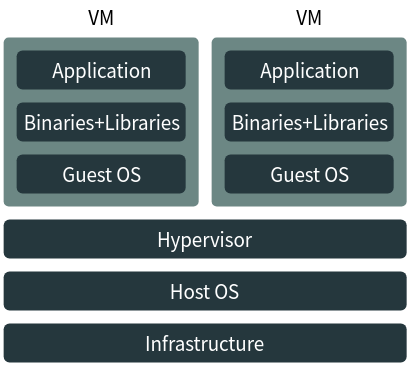
\includegraphics[width=100mm, scale=0.6]{Images/VM_Illustration.png}
      \caption{Components of a Virtualised Environment} 
      \medskip
	  \small
		A conceptual diagram showing the components of a virtualised environment. Original source: Boolean World. \cite{ContainerAndVMImageSource}
\label{fig:VMConceptualDiagram}
\end{figure}

VMs are relatively heavyweight and expensive to maintain, since each separate VM maintains its own operating system (OS) image\footnote{An OS image is system image is a copy of the entire state of an OS stored in a persistent, non-volatile form. It is a package that contains all of the information required to run the OS on the machine, and is usually relatively large as a consequence.}: An overhead in memory and storage footprint. This lack of flexibility also limits the portability of applications that run on virtual machines between different hosting solutions: It is difficult to replicate the same environment configuration on a second VM.

However, VMs allow for multi-tenancy on a single piece of physical hardware, as well as fine-grained resource allocation. 

\subsection{Platform-as-a-Service}
The idea of PaaS is that users are able to focus on running and developing applications instead of managing the infrastructure that supports them. PaaS systems mean that a virtual infrastructure is provided and users can deploy any application on it without needing to worry how resources are allocated to it.


\subsubsection{Containers}
%Containers are disposable, stateless execution environments for applications.
A container is an isolated execution environment defined by a single package that includes everything needed to run it: Code, runtime, system tools, system libraries, settings. They are type of OS-level virtualisation, isolating an application from the host infrastructure on which it is being run: They are almost completely host-agnostic\footnote{Host-agnostic in this context refers to the fact that containers do not have an affinity to any particular host system.}. An application and all of its dependencies can be packaged up in a \textit{container image} that can be published in a \textit{container registry} so that unlimited numbers of users can work in identical application environments.

\begin{figure}[ht]
      \centering
      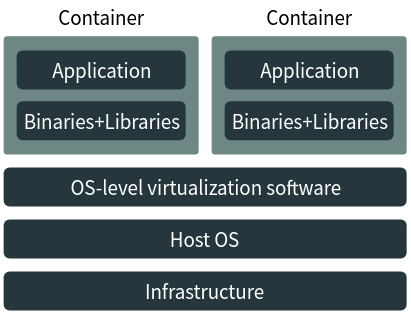
\includegraphics[width=100mm, scale=0.6]{Images/Container_Illustration.png}
      \caption{Components of a Container Environment} 
      \medskip
	  \small
		A conceptual diagram showing the components of a container. Original source: Boolean World. \cite{ContainerAndVMImageSource}
      \label{ContainerConceptualDiagram}
\end{figure}


For setting up a standard application environment and deploying a large number of instances on-demand, containers are simple to configure and much faster to launch than VMs. Among the many advantages of using containers compared to VMs are the following: 
\begin{enumerate}
\item Hosting a container does not include anywhere near the same storage overhead as a VM: Containers do not need to maintain their own copy of the OS image, since they share the kernel of the host OS.
\item All dependencies required by an application are packaged into a single, replicable image. This means that the portability of application environments that is so difficult to achieve with VMs, is native in containers.
\item Containers come with their own separate network stack and storage without the overhead of building and running a VM. 
\end{enumerate}

Many organisations are migrating their infrastructure deployments from VMs to containers. A recent example of this is Netflix, who started migrating their infrastructure hosting to the AWS cloud in 2008. At the time of writing in 2018, Netflix are migrating the hosting of all of their applications from VMs to containers. In a paper discussing this shift in Netflix's infrastructure approach, \cite{NetflixContainerMigration} Leung \textit{et al.} state that ''one of the benefits of using containers ... is that it abstracts much of the machine-centric management that applications were doing in VMs''. This is one of the notable benefits of using containers over VMs: Those deploying the application no longer need to concern themselves with the environment specifics, and get the opportunity to focus on building and running applications.


%\subsubsection{Microservice Architectures}
%Microservice architecture design is an increasingly popular design for distributed systems on all levels, moving away from failure-prone monolithic designs of the past. 


%* granular resource management 
%* loose coupling of services
%* Greater ability to scale

%Microservice architectures also have strengths from a network security perspective by providing air-gapping. An air gap is security measure employed in networks that isolates components of a system from insecure or untrusted components of the system. By isolating functionally separate parts of a system from each other, the number of components of the system immediately affected by a single compromise is minimised and can be confined more easily. From the perspective of performance, it eliminates the possibility of a ''single point of failure'',  reducing the exposure of the overall system to compromise.

\subsubsection{Security through Containerisation} \label{SecurityThroughContainerisation}
%% A lot of this will be covered in the design chapter
An area where much work remains to be done is in bringing security applications into the progressively more popular container ecosystem. There is tremendous potential for the containerisation of security applications, and a number of identified benefits of this approach are described below.

\begin{itemize}
\item \textbf{Disposability}

A major selling point of containers is that they are virtually disposable. In the event that a container becomes infected with malware, it is straightforward to remove it entirely and re-deploy it with minimal disruption to the system. 

\item \textbf{Isolation}

One of the key features of containers which has contributed to their widespread adoption is the ability to restrict and isolate application environments. 

	\begin{itemize}
    \item Containers leverage a Linux functionality known as ''namespaces'', placing applications that run on them in restricted environments, isolated from each other. Individual containers are run in their own independent namespace, and are given their own independent view of a  variety of operating system resources. 

	\item Containers can also be restricted such that any ''root user privileges'' do not have to correspond to the root user privileges on the host machine: The definition of ''root user privileges'' is completely separate from those of the host. 
    
    \end{itemize}
    The net impact of this isolation on the security of containers is that the applications running inside one container will not interact, unless explicitly configured to do so, with applications inside another container or on the host machine. This is a substantial increase in security compared to running multiple non-containerised applications on the same system, and means that even if one container is compromised by malware, the others can continue to operate. This loosely-coupled approach to operating services has the capacity to deliver greater fault tolerance and scalability in systems in which they are deployed, reducing the exposure of the overall system to compromise.
\item \textbf{Standard Base OS Images}

Containerised solutions benefit greatly from being able to build customised containers off standard, widely-used OS images. These standard images benefit from ongoing security auditing and patching, making them a secure foundation for building customised containers. 

\item \textbf{Customisability}

Containers are highly customisable, and enable fine-grained control for system administrators. It is possible to restrict everything from the privileges to the runtime services, enabling restriction of what resources can be accessed by any given container. 

\end{itemize}

In an infrastructure ecosystem where services are increasingly being containerised, the containerisation of security applications is a must in order for them to remain compatible with these new architectures. However, the introduction of new technologies into systems will always bring additional security risks, something that must be carefully considered by organisations migrating their operations to container-based architectures. \cite{7742298} 



%%
%% SECTION 4: CLOSELY RELATED WORK
%%

\section{Closely Related Work} \label{CloselyRelatedWork}


The closely related projects described in this section are explored from the point of view of their most interesting characteristics rather than the achievement of their respective research objectives.
%TODO a little explanation of what the reader should find in this section.


\subsection{Adaptive Honeypots} \label{RelatedHoneypotProjects}

The goals of honeypot deployments can vary greatly, and most honeypots offer a wide variety of options and different functionalities in order to provide flexibility to this end. As identified in \textit{Section \ref{HoneypotDesignSoA}}, increasing the interaction capabilities of a honeypot results in more extensive and detailed information but also more potential damage to the system. Different trade-offs in honeypot design are clearly more suitable for some deployment scenarios than others.

At the time of writing, there were over 1,000 open-source honeypot projects listed publicly on GitHub\footnote{On 24th March 2018, a search for the query 'honeypot' provided 1,405 repositories as results.}. These range from open-sourced production honeypots to major open-source collaborations and hobbyist projects. Research honeypots discussed in journals and conference papers add even more to this number, and there is little doubt that many proprietary production solutions also exist. \cite{CanaryThinkst}

Some of the more significant honeypot projects encountered during this research are described below. These include research honeypots and community-based honeypot developments.% and open-sourced production honeypots.



\subsubsection{Kippo} \label{AboutKippo}
	
	Kippo is an open-source SSH honeypot written in Python which is no longer under active development. It is a medium-interaction honeypot developed by an online development community, and is designed to capture the entire session interaction of an attacker. \cite{KippoHoneypotGithub} It emulates a Debian Linux installation, and provides a wide variety of features as follows:
    
    \begin{itemize}
    \item Kippo provides an out-of-the-box configurable file system and shell for each attacker to interact with. It does not limit the number of simultaneous sessions, and can present a mock file system and shell to each attacker independently.
    \item Kippo implements a falsified SSH service to which attackers can connect.
    \item Kippo includes configuration options for permitted usernames and password combinations which can be controlled by the user.
    \item All interactions with Kippo are logged, including brute-force login attempts, source IP addresses, attacker protocol information, commands executed and records of any attempted downloads.
    \end{itemize}	
	 The fact that Kippo is implemented as a Python application means that attackers will not interact directly with the underlying OS, adding an extra layer of protection for the host system. The fact that it doesn't call on any external software for its core operations makes it much less vulnerable to third-party compromises. 

	Kippo does not have the capability to execute malware, but can be used in conjunction with other solutions such as Cuckoo Sandbox\footnote{Cuckoo Sandbox is an open-source malware analysis system, which allows malicious files to be executed inside an isolated environment in order to analyse their behaviour and properties. \cite{CuckooSandbox}} in order to execute and analyse malware safely in a controlled environment.

Unfortunately, Kippo is an example of a honeypot which is susceptible to fingerprinting due to the fact that it emulates a real system: In its emulation of the OpenSSH service, it is possible to trigger characteristic responses identifying the device as a Kippo honeypot using carefully crafted messages. \cite{Nawrocki2016} This flaw led to the eventual cessation of active development on the honeypot, rendering it largely unusable in the development of new honeypot-based solutions.
	
	\subsubsection{Cowrie} \label{AboutCowrie}
	
	Cowrie is a medium-interaction honeypot which was originally forked from the Kippo project by security researcher Michel Oosterhof. It is actively maintained and supported by a dedicated community, who provide quick response times to queries and bug-fixes. It is widely used in both research and production projects as a medium-interaction honeypot. \cite{PickyAttackers2017} \cite{TPotWebpagev17} \cite{ModernHoneyNetworkLaunchAnnouncement} 
    
	In addition to the capabilities and features provided by the Kippo honeypot, Cowrie has some additional features \cite{CowrieGithub} \cite{CowrieWebsite} including but not limited to the following:
	
	\begin{itemize}
		
		\item Cowrie enables attackers to gain access to the honeypot using an emulated telnet client as well as SSH, supporting the two protocols which are most widely-targeted by IoT botnets. \cite{UnderstandingTheMiraiBotnet} \cite{HajimeMysteriousBotnet}
		
		\item Cowrie logs all attack session information in JSON format, which is a widely-used format that can be processed by many tools;
        
        \item Cowrie provides integration with a number of useful tools including VirusTotal malware database and the Mailoney SMTP honeypot;
        
		\item Cowrie also improves substantially on its predecessor, Kippo, resolving many of the major fingerprinting issues.
	\end{itemize}

    Interestingly, there is also some activity with respect to containerisation of the Cowrie honeypot. A basic Cowrie container image has been developed by contributors to the Cowrie project, \cite{DockerCowrie} which illustrates an increasing awareness of the need to migrate security applications into container-driven architectures.
	
	\subsubsection{Honeyd} \label{AboutHoneyd}
    
    Honeyd is an important predecessor to many of today's honeypots, and is likely the best-known honeypot implementation. It is an open-source, virtualised low-interaction honeypot released originally in 2002, and is currently in maintenance mode. It was originally developed by Niels Provos. 
    
     Honeyd is flexible and adaptive in that it can be configured both to run arbitrary services and to advertise itself as running different operating systems, learning the service ''personalities'' by reading Nmap fingerprint files in order to mimic them. \cite{HoneydWebsite} It cannot however emulate system components such as file systems or command execution. As explained in an article \cite{ProvosHoneyd} by creator Niels Provos, Honeyd ''listens to network requests destined for its configured virtual honeypots'' and ''responds according to the services that run on the virtual honeypot. Before sending a response packet to the network, the packet is modified by Honeyd's personality engine to match the network behaviour of the configured operating system personality.'' 

Additional features of Honeyd include the ability to create virtual routing topologies, and the ability to enhance configured routes with realistic latency and packet loss characteristics in order to appear more convincing. Though it has provided inspiration for finding adaptive solutions for honeypots, the fact that it is no longer being actively developed renders it largely unusable in new deployments.

\subsubsection{IoTPot} \label{AboutIoTPot}
	
	IoTPot is a research honeypot developed by Yin Minn Pa Pa \textit{et al.}, which they describe as ''a novel honeypot that emulates interactions of the telnet protocol and a variety of IoT devices''. \cite{IoTPot2016} It is a reactive IoT honeypot that targets the study of telnet-based attacks.  It is particularly interesting because of its ability to react to the requests sent by attackers, providing them with a dynamically generated response deemed to be most likely to match the CPU architecture of the system that is being targeted in the attack. 
    
\begin{figure}[ht]
      \centering
      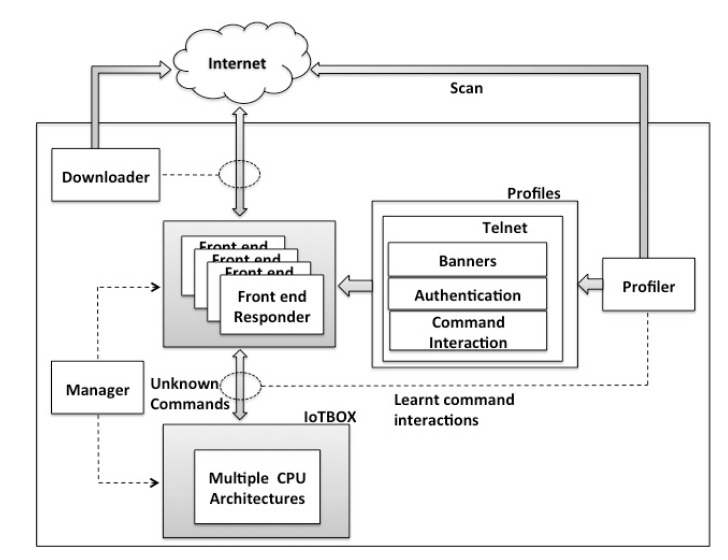
\includegraphics[width=150mm, scale=1]{Images/iot-pot-sys-arch.PNG}
      \caption{The IoTPot Honeypot Architecture} 
      \medskip
	  \small
		This diagram is originally from a paper published by the researchers who developed the IoTPot honeypot, and illustrates the operation of the IoTPot system. \cite{IoTPot2016} 
\label{fig:Images/iot-pot-sys-arch.PNG}
\end{figure}
    
    IoTPot was designed in recognition of the fact that there are too many different types of IoT device to be able to develop honeypots for all of them. The principles behind the operation of IoTPot are very much based on a honeypot network called SGNET, where low-interaction sensors forward attacks that they receive to a high-interaction honeypot to handle. \cite{SGNET} This is similar to the function of the \textit{front-end responder} in IoTPot, which is the component of the system that interacts directly with attackers. A diagram of the system architecture can be seen in figure \ref{fig:Images/iot-pot-sys-arch.PNG}.
    
    \begin{itemize}
    \item The \textit{front-end responder} component deals with negotiating the Telnet protocol with an attacker based on what it believes they are looking for. It emulates a number of different device profiles, and for each device profile deals with authentication attempts, command interactions and emulation of device-specific telnet options.
\item If a command is issued by the attacker that the \textit{front-end responder} doesn't know how to handle, it connects via Telnet to the \textit{back-end responder}, a component called \textit{IoTBox}. This component contains emulated operating systems for a number of different CPU architectures, meaning that the command can be executed on each of these and an appropriate response returned to the attacker as a result.
    \end{itemize}
     
    Most honeypots are far more passive in their approach to handling incoming commands from attackers, and are incapable of providing any more than one valid response to a given request. At the time that it was developed, the researchers claimed that there existed no other IoT honeypot ''that can mimic IoT devices of many different CPU architecture while listening on 23/TCP with the ability to learn unknown command interactions.'' 
    
    As an adaptive telnet honeypot, IoTPot appears to be very effective. However, it is relatively restricted in that it can only deal with telnet-based attacks, limiting the attacks it can capture. According to the paper, the researchers ''plan to extend IoTPot to support more protocols that are likely the target of attacks'' in the future.

	
	\subsubsection{IoTCandyJar} \label{AboutIoTCandyJar}
IoTCandyJar is a recent IoT honeypot developed by Luo \textit{et al.} who classify it as an \textit{intelligent-interaction} honeypot rather than as low, medium or high-interaction. \cite{IoTCandyJar} The researchers explain that ''the goal of intelligent interaction is to learn the 'correct' behaviors to interact with clients from zero knowledge about IoT devices''. Their approach is to utilise machine learning techniques to determine the most appropriate tactics to prolong attacks.

The IoTCandyJar honeypot is composed of a number of primary modules, which can be seen in figure \ref{fig:Images/iot-candy-jar-sys-arch1.PNG} as follows:
\begin{itemize}
        \item The \textit{IoTScanner} module leverages the fact that there are powerful scanning tools freely available to identify IoT devices, using \textit{Shodan, Censys, Masscan} and \textit{Zoomeye} scanning tools to identify IoT devices on the internet. It actively probes these devices, collecting their responses to various requests that have previously been captured by IoTCandyJar. 

        \item The \textit{IoTLearner} module builds intelligence into the honeypot, using the responses captured by the \textit{IoTScanner} module to train a model using machine learning algorithms. The accuracy of the responses provided to requests improve with increasing numbers of interactions with attackers: If an attacker sends a second request after receiving a response from IoTCandyJar, the response is deemed to have been correct.

      \item The \textit{IoTDatabase} stores all of the captured requests and responses, and stores any information relating to the machine learning model.
\end{itemize}    

\begin{figure}[ht]
      \centering
      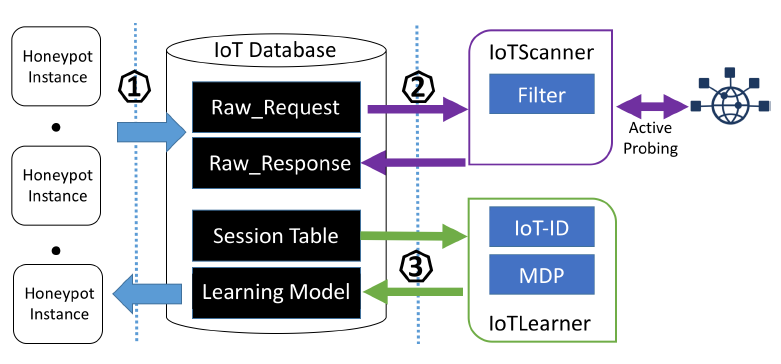
\includegraphics[width=150mm, scale=1]{Images/iot-candy-jar-sys-arch1.PNG}
      \caption{The IoTCandyJar Honeypot Architecture} 
      \medskip
	  \small
		This diagram is originally from a paper published by the researchers who developed the IoTCandyJar honeypot, and illustrates the operation of the IoTCandyJar system. \cite{IoTCandyJar} 
\label{fig:Images/iot-candy-jar-sys-arch1.PNG}
\end{figure}

The major selling point of IoTCandyJar is the dynamic approach that it takes to reacting to probing by IoT botnets. Similarly to IoTPot, IoTCandyJar aims to provide the best response to an attacker based on what they are determined to be seeking. The major difference between these two honeypots is in the approach they take to achiev this: Where IoTPot determines the most appropriate response by generating the correct response through execution of the request, IoTCandyJar learns the best response to a request based on interacting with attackers. Responses to attacker requests are generated based purely on what the system has learned from previous interactions with attackers, and not through any execution of requests. \cite{IoTCandyJar}

    
  	\subsubsection{Zigbee Honeypot} \label{AboutZigbeeHoneypot}
    Dowling \textit{et al.} developed a research honeypot targeted at attackers of Zigbee devices, which are devices commonly used in WSNs. \cite{Dowling2017} The development of this honeypot was motivated by the fact that as these IoT devices are being more widely-deployed and their vulnerabilities are also becoming well understood: Therefore, an assessment of the threat to these devices is essential.
      
    In their implementation of the honeypot, Dowling \textit{et al.} included a number of interesting measures to initiate the interest of attackers in the honeypot:
    
    \begin{itemize}
    \item The host name for the honeypot was configured to be \textit{zigbee-gateway} as a means of assessing whether there is any awareness of Zigbee devices amongst attackers;
    \item The researchers implemented a means of transmitting of fictitious medical traffic, which is transmitted in cleartext over an unfiltered network. 
    \end{itemize}
    
    The generation of potentially interesting network traffic in order to entice attackers to attack the honeypot is a thought-provoking feature of this solution. Though the research conducted is largely focused on identifying whether there is any awareness of Zigbee devices specifically, the idea of adapting the honeypot to the attackers it wishes to attract is a useful one.   
  

\subsection{Containerised Honeypots} \label{RelatedHoneynetProjects}
Related projects identified in the domain of containerisation of honeypots are limited in number, primarily because the security domain is still catching up with the migration of infrastructures to container-based architectures. The research conducted in these related projects focus on both the benefits of using containers for hosting honeypots, and the challenges that are faced in doing so.

	\subsubsection{Distributed Virtual Honeynets} \label{AboutDistributedVirtualHoneynets} 
    In 2014, Pisarcik \textit{et al.} developed a distributed honeynet of high-interaction honeypots using containers for OS-level virtualisation, an approach which at the time was relatively unexplored in research. \cite{Pisarcik:2014:FDV:2659651.2659685} Their motivations for developing such a solution were:
    \begin{itemize}
    \item The fact that administering honeypot-driven systems is time-consuming, motivating the use of containers to simplify their management; and
    \item The ability of honeypots to correlate attack events in order to determine whether they are localised or distributed in nature, quickly allowing for identification of attack trends.
    \end{itemize}
    
    Though the approach to designing and evaluating their honeynet solution is worthy of note, the more significant contribution made by this research is in relation to the containerisation of honeypots and honeynets. The research highlights that when compared to virtual machines or bare-metal systems, OS-level virtualisation incurs very little performance or maintenance overhead. \cite{Pisarcik:2014:FDV:2659651.2659685} As well as this, they note that using containers adds an additional layer of deception to honeypots: Since they are isolated environments sharing the kernel of a real OS, they are more likely to appear as a legitimate system when fingerprinted. 
    
    All of these features would make it seem that containers are a perfect deployment solution for honeypots: However, they also address the potential security pitfalls of using containers to host honeypots, particularly because of the risk to the host system by virtue of sharing its OS kernel with containers. These are interesting insights regarding the practicality of using containers in honeypot-driven solutions.

   
    \subsubsection{Using Linux Containers for Deceptive Honeypots} \label{AboutDeceptiveHoneypots}
    In a paper published in 2017, Kedrowitsch \textit{et al.} explore the use of Linux-based containers (LXCs) in honeypot deployments. \cite{LXCsForDeceptiveHoneypots2017} However, the use of LXCs here is examined from the perspective of their ability to evade detection by malware, which has often been found to change its behaviour after detecting a VM-based environment. \cite{SpotlessSandboxes} The motivation behind this is to identify whether container environments will be feasible in the long term as an approach to hosting honeypots without being detected by malware.

The researchers performed a number of experiments where they compared the fingerprinting weaknesses of LXCs to those of bare-metal systems and VMs. They focused on the typical techniques that malware employs in fingerprinting VMs: Comparing the response generated for a particular input against the response that would be expected from a bare-metal system. In particular, they chose to test and compare the following properties of VMs and containers as a means of fingerprinting:

\begin{itemize}
    \item Variability and execution time in CPU clock sampling;
    \item Reported CPU information;
    \item Instruction execution time.
\end{itemize}

When evaluating their experiments, it was found that containers were much less susceptible to fingerprinting than their VM counterparts, which was expected due to the fact that LXCs are executed directly on bare-metal hardware as isolated processes whereas VMs are not. However, it was strongly concluded that if a malware author wanted to detect a container environment as a means of fingerprinting a system, they would have no difficulty in doing so. 
    

\subsection{Honeypot-Driven Cyber-Incident Monitors} \label{RelatedIncidentMonitorProjects}
Projects listed in this section are relevant since they make the use of honeypots much more accessible to individuals and organisations. They recognise the importance of data aggregation and visualisation from multiple honeypots in order to provide important data to key decision makers, encouraging the use of active network defence by making it much easier to manage and benefit from.

	\subsubsection{TraCINg} \label{AboutTraCINg}
    
    TraCINg is a honeypot-driven cyber incident monitor developed by academic researchers Vasilomanolakis \textit{et al.} in 2015, \cite{Vasilomanolakis}. Its development was motivated by the observation that the consolidation of data gathered from honeypots in different deployment contexts can allow attack data to be correlated, enabling the identification of emerging outbreaks of related attacks. 
    
    The TraCINg system gathers data from a large number geographically distributed honeypots with the aim of correlating attack events. Many of these honeypots are deployed on cloud platforms, which was the approach determined by the researchers to provide the greatest diversity of deployment locations and maximum system uptime for uninterrupted monitoring. Arbitrary open-source honeypots can be used with the TraCINg system, provided that their data is logged in JSON format.
    
   This incident monitoring solution is not intended to be highly deployable or low-cost for use in production systems, but addresses the consideration of aggregating and summarising complex data in a meaningful manner through visualisation, enabling the succinct description of important data for key decision-makers. Their proposal for correlation of data from large deployments distributed honeypots is very interesting: However, their solution uses two low-interaction honeypots, limiting the level of detail of the attack data captured. An improved system would be able to capture more data about attack events in order to gain greater insights into the motivations and methods of attackers.

  
    \subsubsection{TPot} \label{AboutTPot}
    The TPot project is a honeypot-based incident monitor that was developed by Deutsche Telekom, and which they use in their production networks for early threat detection. They decided to open-source their development with the aim of making the deployment of honeypots in production networks more feasible for organisations. \cite{TPotWebpagev17}
    
    TPot supports multiple open-source honeypots hosted in containers. The system consists of a number of components, the most relevant of which are listed as follows:
    \begin{itemize}
    \item \textbf{Containerised Honeypots}

	The TPot system leverages the benefits of containers listed in \textit{Section \ref{SecurityThroughContainerisation}} in order to provide a highly deployable honeypot system. The containerised honeypots supported by the TPot platform are all actively maintained and target a variety of different interactivity levels and attackers\footnote{The honeypots supported by the TPot platform at the time of writing are Conpot, Cowrie, Dionaea, Elasticpot, eMobility, Glastopf, Honeytrap, Mailoney, rdpy and VNClowpot. \cite{TPotWebpagev17}}.

        \item \textbf{The ELK Stack}
    
    The Elasticsearch-Logstash-Kibana (ELK) stack is a collection of log management tools that perform search, logging and visualisation functions respectively. In TPot they are used to analyse, index and represent logged attack data captured by the honeypots.

    \end{itemize}
    
    \begin{figure}[ht]
      \centering
      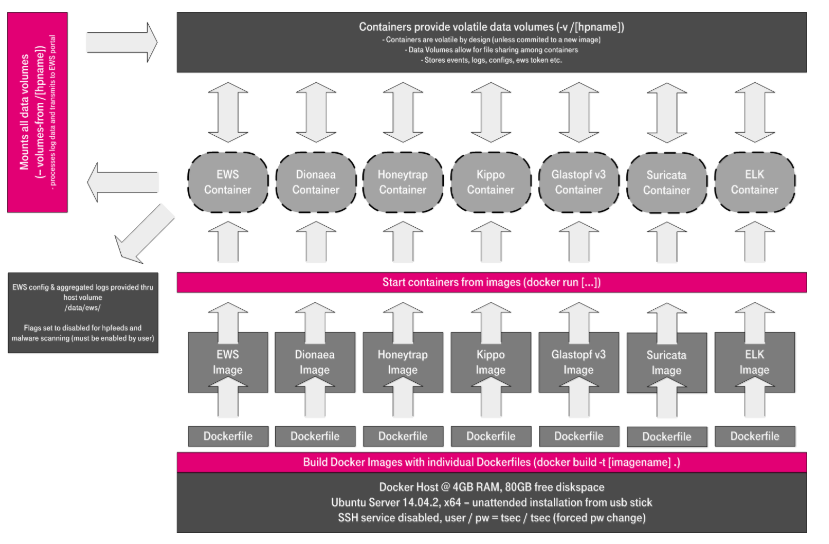
\includegraphics[width=160mm, scale=1]{Images/t-pot-diagram.PNG}
      \caption{Diagram of the TPot Architecture} 
      \medskip
	  \small
		This diagram is provided by the developers of the TPot project as an explanation of the operation of the system. \cite{TPotWebpagev16} Each honeypot is defined by a \textit{Dockerfile}, which is built into an \textit{image}. This image is then used to run the honeypot, and data generated by the honeypot is stored in volumes shared with the host system. The data can then be passed to other systems such as Deutsche Telekom's in-house data aggregation tool \textit{EWSPoster} as shown. 
\label{fig:Images/t-pot-diagram.PNG}
\end{figure}
    
    An infographic provided by the TPot developers can be seen in figure \ref{fig:Images/t-pot-diagram.PNG}. All container images for the honeypots are built based on the Alpine Linux\footnote{Alpine Linux describes itself as a security-oriented, lightweight Linux distribution based on \textit{musl}, \textit{libc} and \textit{busybox}.} container image, which has a particularly small image size meaning that its storage footprint is minuscule. A benefit of running the honeypots inside containers that the developers highlight on their webpage is that they can ''run multiple honeypot daemons on the same network interface while maintaining a small footprint and constrain each honeypot within its own environment''. \cite{TPotWebpagev16}

The proposition of leveraging the benefits of containers in order to host honeypots is an intriguing one, particularly since the difficulties of deploying and maintaining honeypots have been a huge barrier to their widespread adoption to-date. The work on this project by Deutsche Telekom strengthens the case for the coupling of containerised honeypot deployments and visualisation tools.
    
    \subsubsection{Modern Honey Network} \label{AboutMHN}
    The Modern Honey Network (MHN) is a production system developed by Anomali Inc. to manage enterprise honeypot deployments. Their decision to open-source the system was motivated by similar reasons as those given by the TPot developers, being that the deployment and maintenance of honeypot deployments has always been ''a complicated process reserved for security companies and security researchers.'' \cite{ModernHoneyNetworkLaunchAnnouncement} The result is that the MHN simplifies the process of deployment and management of honeypots, making it more feasible for organisations to use active network defence.
    
    The MHN is a centralised server system which is concerned with managing the deployment of honeypots as well as the aggregation of their data. It has support for a large number of open-source honeypots, including the Cowrie honeypot\footnote{The full list of supported honeypots is as follows: Amun, Cowrie, Conpot, Dionaea, ElasticHoney, Glastopf, Shockpot, and Wordpot. MHN also supports threat detection tools including Snort, Suricata and p0f.}. All of these honeypots are low or medium interaction open-source honeypots, which the MHN team say were selected to minimise the risk associated with a deployment of honeypots in a production environment. Honeypot data collected by the MHN system can be visualised with Splunk, a data analysis and visualisation tool: However, unlike TPot's support for the ELK stack, Splunk is not shipped as part of the MHN system.

    
\section{Summary} \label{SoASummary}
Based on the background provided in this section, it is obvious that the field of cybersecurity is dynamic and full of challenges. As aptly phrased by Fred Schneider, ''like good health, cybersecurity is never going to be a \textit{solved problem}''. 

Many of these challenges are the result of gross negligence on the part of manufacturers and system designers; Others are due to obvious oversights and mistakes resulting from a lack of usability; Yet others are a consequence of not understanding the implications that insecure technologies can have for privacy and safety. What all of these present is an opportunity for improvement of current approaches to the implementation of technologies and connected systems.

The work done by those researchers and developers behind the \textit{closely related projects} described in \textit{Section \ref{CloselyRelatedWork}} indicates the awareness and interest that exists around tackling the challenges that are being faced in the security of modern systems. It is a similar interest and awareness on the part of the author which motivates the decision to improve on the current state of the art in this area.

             %% STATE OF THE ART   
\chapter{Problem Formulation} \label{Chapter3}

As discussed at length in \textit{Chapter 2}, the rapid advancement of security threats in response to technological developments and innovations makes it crucially important for mitigation techniques and tools to keep pace. One thing is abundantly clear: That there is an urgent need for re-evaluation of current best-practice in cybersecurity defences, particularly for critical service infrastructures whose general lack of implemented security mechanisms is positively dangerous. It is this consideration that is at the heart of formulating objectives for this research.

\textit{Section \ref{IdentifiedChallenges}} explores a number of the major challenges identified in \textit{Chapter 2}, seeking out the heart of the issues and hypothesising about how these can be resolved in tandem.

\textit{Section \ref{ProposedWork}} addresses the identified challenges in the formulation of proposed work for this research, and outlines the basis of the research objectives. How these research objectives will be addressed in practise is the subject of \textit{Chapter 4}.


%
%
% 	SECTION 1: CHALLENGES IDENTIFIED
%
%

\section{Identified Challenges \label{IdentifiedChallenges}}

A number of challenges currently facing the security of modern infrastructures and systems were explored in \textit{Chapter 2}. The challenges found to be of most interest to this research are outlined in the following subsections.


\subsection{Incident Monitoring in Critical Service Infrastructures}
As explained in the context of the WannaCry ransomware attacks on the NHS in \textit{Section \ref{WannaCryNHSCase}}, IT systems in many organisations are comparable to a \textit{black-box system}\footnote{This is a term commonly used in control systems theory meaning that the inputs and outputs of a system are known whilst the internal workings are not.}, an illustration of which can be seen in figure \ref{fig:Images/black_box.png}. Such a system gives no indication of what is happening internally until it begins to behave unexpectedly, meaning that when issues arise they are difficult to diagnose and almost impossible to resolve. However, ineffective feedback mechanisms are often as bad as having no mechanism in place: Passive mechanisms like firewalls are imprecise in their suspection of malicious activity, meaning that when a significant event does occur it can easily go unnoticed. \cite{Voronkov:2017:SLR:3161158.3130876} It is crucially important that \textit{effective} feedback mechanisms are employed which are simple to use and capable of communicating key information to those who can act upon it.


%\includewidefigure{Images/black_box.png}{Illustration of a Black-Box System}{An illustration of a black-box system, where a known input \textit{f(x)} is provided to the system, unknown operations are performed on it, and a known output \textit{g(x)} is generated as a result.}{Images/black_box.png}

\begin{figure}[ht]
      \centering
      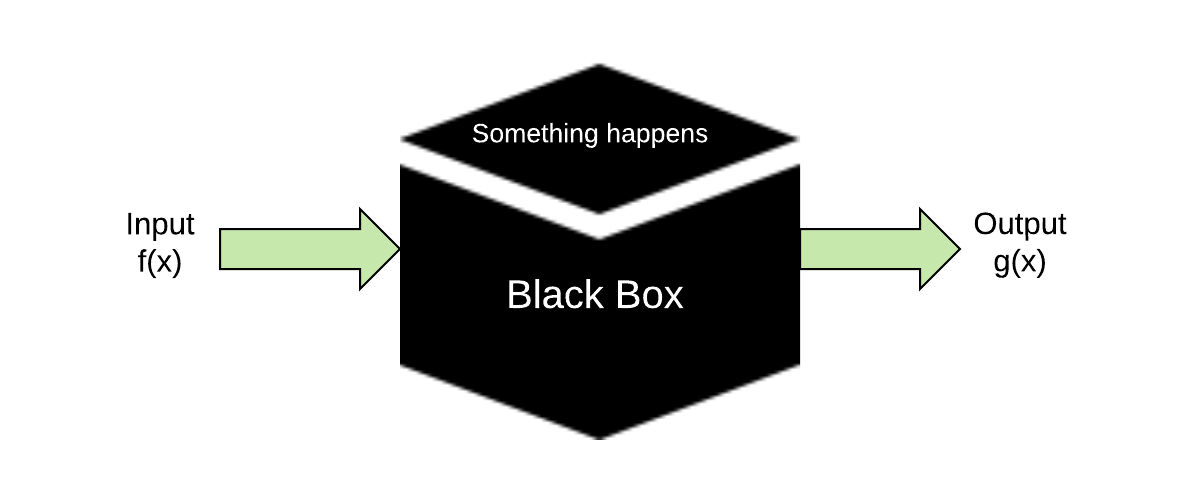
\includegraphics[width=175mm, scale=1]{Images/black_box.png}
      \caption{Illustration of a Black-Box System} 
      \medskip
	  \small
		An illustration of a black-box system, where a known input \textit{f(x)} is provided to the system, unknown operations are performed on it, and a known output \textit{g(x)} is generated as a result.
\label{fig:Images/black_box.png}
\end{figure}

It is obvious that in order to implement effective threat mitigation mechanisms, the most relevant risks to that system must first be understood: Something that was highlighted in an interview with Stuart Reed, senior director at NTT security, who argues that ''the best starting place is to understand where... risks come from''. \cite{MANSFIELDDEVINE201716} To illustrate this, consider critical service infrastructures such as the NHS: These are most at risk from those with a political motivation to do damage to a nation-critical infrastructure, such as nation-state attackers. While such infrastructures generally rely on firewalls which may protect against script-kiddies and other unsophisticated attackers, nation-states generally employ sophisticated technical attackers who are capable of discovering entirely new flaws and exploits in systems. This motivates and highlights the need for a technology that is able to provide intelligence on these active, dynamic threats for critical service infrastructures.


\subsection{The Need for Active Defence Mechanisms}
%As has been highlighted by their success in a number of the \textit{closely related projects} in \textit{Section \ref{CloselyRelatedWork}}, 
As discussed in \textit{Section \ref{ChallengesForFirewalls}}, although the use of passive intrusion detection technologies such as firewalls hold an important place in securing IT systems, they have limited diagnostic capabilities since they can only mitigate against \textit{known threats}. In an analogy comparing cybersecurity to health, Fred Schneider explains that ''as with medical problems, some attacks are best addressed in a reactive way''. \cite{Schneider11_BlueprintForScienceOfCybersecurity} 

Honeypot-driven solutions are promising in what they can offer with regards to active network defence and rapid incident response. Modern IT infrastructures are sorely in need of such \textit{adaptive} approaches to defence: Defence mechanisms that, in the face of uncertainty about the nature of attacks, can continue to provide threat mitigation. It is clear from the discussion provided in \textit{Section \ref{HoneypotsSection}} that honeypot solutions have the ability to address this requirement.

\begin{itemize}
\item The information that honeypots can capture enables continuous improvement of infrastructure design and defences;
\item The low number of false positives that result from honeypots make identifying threats straight-forward: All logged events can generally be assumed to be threats;
\item Honeypots are capable of alerting first-responders to highly-probable threats as soon as they occur, enabling rapid response before an attack has the opportunity to spread.
\end{itemize}

However, these benefits are identified in recognition of the fact that the widespread deployment of honeypot-based systems to-date has been impeded by the maintenance overhead that they incur for system administrators, as was identified by the developers of Deutsche Telekom's TPot as outlined in \textit{Section \ref{AboutTPot}}. In order for such a system to be practical and feasible to deploy in a production system, it must be:

\begin{enumerate}
    \item Inexpensive to deploy, operate and maintain;
    \item Effective and reliable in securing a network;
    \item Simple to use.
\end{enumerate}
    
In order to be viable for widespread adoption as a security service, a honeypot-based deployment solution must address all of these requirements.
	
\subsection{The Effectiveness of Honeypots in Enticing Attacks}
%This is in relation to how effectively honeypots are designed in order to entice attacks, which is a crucial element to their success.
As identified from the closely related work explored in \textit{Section \ref{CloselyRelatedWork}}, although there has been excellent progress made in the enhancement of honeypot design so that attack sessions are prolonged and more attack data is captured for analysis, there is little conclusive research found regarding how to enhance the design of honeypots in order to initiate the interest of attackers. 

In almost all research found, there was a heavy focus on encouraging the prolonged interaction of attackers with honeypots rather than on attracting that interaction in the first place. \cite{CowrieWebsite} \cite{IoTPot2016} \cite{IoTCandyJar} \cite{Dowling2017} Dowling \textit{et al.} explored some interesting measures to entice attackers seeking to compromise Zigbee devices, but the impact that these measures had on the number of attacks attracted was not a metric of interest in their research. \cite{Dowling2017}

The effectiveness of honeypot-based technologies in defending systems is influenced greatly by their ability to attract attacks away from valuable systems in the environment they serve to protect. Understanding how honeypots can be designed to be as irresistible as possible to attackers would further their adaptivity in rapidly alerting first responders to the fact that they have been attacked, allowing action to be taken before a subsequent attack is targeted at valuable systems.


%
%
% 		SECTION 2: PROPOSED WORK
%
%

\section{Proposed Work} \label{ProposedWork}

It is clear that taking an active approach to mitigating risks to critical service infrastructures is the way forward, and that the capabilities of honeypots can aid greatly in achieving this. Though there are a number of existing approaches both in research and production outlined in \textit{Section \ref{CloselyRelatedWork}} that have contributed excellent work towards such a solution, there exists no one solution which can provide a practical, feasible means of employing active network defence as a single networked deployable unit.

Given the challenges identified in \textit{Section \ref{IdentifiedChallenges}}, two research objectives were formulated as a proposal to tackle them.

\subsection{Objective 1: A Honeypot-Driven Cyber Incident Monitor for Critical Service Infrastructures} \label{Objective1}

This objective addresses the need for a feasible active intrusion detection solution to enable rapid response in critical service infrastructures by enabling action to be taken on threats with minimal operational overhead. 

The requirements of such a solution include:

\begin{enumerate}
\item A deployment solution that is cost-effective, quick to deploy and quick to scale, whilst compatible with existing IT infrastructure. 
\item A number of highly-attractive honeypots, which can effectively lure attackers away from valuable machines in the network in which they are deployed. 
\item A centralisation point for data collected from any deployed honeypots, such that administrators may be given a holistic view of their system in order to facilitate them in making quick, well-informed decisions.
\item An effective and reliable alert system, such that the key parties can be alerted as soon as possible after a threat event is detected by the system.
\end{enumerate}

The constituent components of such a system are addressed in the following sections.

\subsubsection{Honeypots for Active Network Defence}
As outlined at length in \textit{Section \ref{HoneypotsSection}}, honeypots enable the identification of vulnerabilities and flaws in the system in which they are deployed and are capable of mitigating against risks that were previously unknown to those administering the system, unlike passive defence mechanisms like firewalls. This makes them an obvious choice for the implementation of active network defence in critical service infrastructures.

In the proposed incident monitoring system, the use of a number of honeypots in a honeynet configuration has been identified as a ideal approach to providing effective incident monitoring. There are multiple benefits of a honeynet-based approach here, including the potential to study attack propagation through a network and the fact that there is an increased honeypot attack surface to distract an attacker away from valuable systems in the same environment. The honeypots in the proposed system would act as sensors, providing a feedback mechanism regarding threat events in the network by logging attack activities for analysis.



\subsubsection{Containerised Honeypots}
Containers have been identified as an effective deployment option for the proposed system, given the properties that were outlined in \textit{Section \ref{SecurityThroughContainerisation}}, since they cater for many of the requirements of a scalable honeypot-based incident monitoring system as outlined in the previous section.

By deploying honeypots in inter-networked containers it becomes possible to provide a flexible, low-cost, low-maintenance deployment solution for organisations. A single container will only use a relatively small proportion of a machine's CPU power and storage, and a number of containers on a single host can use the same physical network interface whilst implementing their own independent network stack. \cite{LXCsForDeceptiveHoneypots2017} Importantly, any container can be deployed and removed with minimal operational overhead because of their portable configuration. In the case of critical service infrastructures, using such an architecture would enable recovery of any containerised component of the system after compromise with minimal downtime. 

From the perspective of overhead and maintenance, containers are an excellent choice as a hosting platform for applications in today's IT infrastructures. The migration of security applications to container-based architectures is both beneficial and essential for organisations hosting their infrastructure in containers: The success of containerised honeypots in the TPot platform illustrates this. \cite{TPotWebpagev17} As well as this, containers enable a degree of reproducibility not usually achievable in computer science research, as pointed out by Cito \textit{et al.}. \cite{ReproducableResearchEnvironmentsContainers} All of these benefits give a strong basis for the use of containers in hosting a honeypot-driven solution. 



\subsubsection{Visualisation of Honeypot-Generated Data}
Analysis of honeypot data is simplified greatly through use of visualisation tools, which enable classification and visualisation of complex attack data in order to make meaningful deductions. 

As part of a honeypot-driven incident monitoring solution, it is clear that information gathered from honeypots would benefit from being aggregated, analysed and visualised in a central management system that consolidates the data and perform processing operations on it before making it available to a user: Both the MHN and TPot projects exemplify this approach. \cite{TPotWebpagev17} \cite{ModernHoneyNetworkLaunchAnnouncement}

Such a management system is a crucial component of the cyber incident monitoring system, where attack data is gathered centrally and made accessible to system administrators who require a holistic view of the state of the system. A management system performing this function should be directly reachable by the honeypots, but obscured from attackers within them.  


\subsubsection{Notification System for Threat Events}
The challenges faced in the aftermath of the WannaCry ransomware infection of NHS systems have illustrated the importance of having a feedback mechanism in place, which is capable of notifying first-responders in the event of undesirable behaviour being detected. An effective cyber incident monitor should provide this feedback mechanism, allowing threat data to be presented to those who can act on it as soon as it is detected.


\subsection{Objective 2: A Proposal for Adaptive Honeypots} \label{Objective2}

It is clear that the effectiveness of honeypots in intrusion detection depends heavily on their design, which in turn depends on the context of their deployment and the value that they are required to deliver. The single point of commonality between all honeypot deployments is that they must be \textit{adaptive} in order to deceive attackers effectively, assisting them in what they believe to be the successful progression of their attack whilst quietly monitoring their actions. 

This need for adaptivity is beginning to be addressed in research more commonly, but there are gaps in current research that have provide an opportunity for improvement. In particular, all of the closely related honeypot projects identified in \textit{Section \ref{RelatedHoneypotProjects}} which address the adaptivity of honeypots focus on approaches to \textit{maintaining} the interest of an attacker, rather than on initiating the interest in the first place. \cite{CowrieWebsite} \cite{IoTPot2016} \cite{IoTCandyJar} Designing adaptive honeypots such that they advertise the most commonly sought-after characteristics of victim systems is a problem of major interest.
% However, IoTCandyJar does not address what characteristics of their honeypots attracted the attackers in the first place: Their implementation is more focused on maintaining interest than initiating it.

%\begin{figure}[ht]
%     \centering
%      \includegraphics[width=100mm, scale=0.6]{Images/Baseline__SoA__proposed_and_optimal_solutions.png}
%      \caption{add caption}
%      \medskip
%	  \small
%		An illustration of the relative improvement that is possible in the design of a solution. In recognition of the fact that the theoretical optimal solution is not attainable, one would strive to improve upon the current state-of-the-art and devise a solution that is as close as possible to the theoretical optimum.
%      \label{TheoreticalOptimalSolution}
%\end{figure}

%\includefigure{TheoreticalOptimalSolution}{Improving upon a baseline implementation}{An illustration of the relative improvement that is possible in the design of a solution. In recognition of the fact that the theoretical optimal solution is not attainable, one would strive to improve upon the current state-of-the-art and devise a solution that is as close as possible to the theoretical optimum.}{Images/Baseline__SoA__proposed_and_optimal_solutions.png}


\subsubsection{Measuring the Effectiveness of Honeypot Characteristics} \label{BenefitsForUsingHoneynetForExperiments}
Conducting a robust evaluation of the effectiveness of particular honeypot characteristics in attracting the interest of attackers is an interesting but difficult problem. The effectiveness of a honeypot is difficult to quantify, but it is clear than an effective honeypot will provide effective intrusion detection and, depending on the context of its deployment, capture relevant attack data in a certain level of detail.

Honeypot effectiveness can potentially be measured through such properties as the number of attacks that are attracted, the number of true positives detected, the ability to deduce attacker motivation based on data captured, etc. \cite{Nawrocki2016} Credible measurement of any of these properties is largely dependent on maintaining a consistent research environment within which relative performance can be evaluated accurately.

A honeynet is an effective way of accurately and simultaneously measuring the appeal of certain characteristics of honeypots in experiments, since multiple characteristics can be trialled in the same environment over the same period of time. By using a honeynet configuration in the research environment, data can be captured from multiple honeypots under the same environmental conditions, and the relative performance based on slightly different configurations can be measured. 


\subsubsection{Targeted Honeypots for the Internet of Things}
From the outset of this research, one of the most interesting and active categories of botnet identified was that of IoT botnets, a revolutionary and recent phenomenon which is cause for serious concern. 

Proposing an approach to designing adaptive honeypots with a focus on making them maximally attractive to IoT botnets would contribute to current knowledge of these attackers by understanding more about their preferred vulnerabilities and target systems. The configurability and informative capabilities of honeypots makes them an attractive option in this regard. Targeting these attackers in the design and implementation of the proposed system would be a valuable additional contribution to the field of security as an application of the cyber incident monitor.





				%% PROBLEM FORMULATION
%%
%%
%%			CHAPTER 4: DESIGN
%%
%%

\chapter{Design} \label{Chapter4}

To meet the research objectives outlined in \textit{Chapter 3}, the requirements defined in \textit{Section \ref{ProposedWork}} must be addressed in the design of the proposed system. With these in mind, an initial system design was devised. 

There are countless factors that must be taken into consideration when designing a research environment, and particularly when a flawed design can have far-reaching implications and consequences for the security of others unaware of the project in the first place. In order to develop solutions that were both secure and effective, every aspect of the design required scrutiny and careful planning. 


\textit{Section \ref{FunctionalConsiderations}} details the \textit{initial} design decisions that were made to address the functional requirements of the research environment.

\textit{Section \ref{DesignChallenges}} addresses a number of identified challenges that required additional analysis to fully satisfy the requirements of the proposed system.

\textit{Section\ref{DesignSummary}} provides a summary, recognising in particular the unpredictable nature of research as it evolves. 

\section{Functional Considerations} \label{FunctionalConsiderations}
This section describes many of the functional design considerations and decisions made relating to the implementation of the research environment. These include initial design decisions regarding the environment deployment platforms, the configuration of the honeynet and the design of the monitoring system.

\subsection{Deployment Platform}
Selection of the hosting infrastructure and platforms for the proposed system was an important consideration in the design which would have a significant impact on the successful development of cyber-incident monitor as well as on the design proposal for adaptive honeypots.

\subsubsection{Choice of Hosting Solution}
%% Should talk about the considerations of hosting it on a local machine (cost, isolation from personal networks and devices a consideration)
The benefits of outsourcing the hosting of services to a third-party cloud platform were discussed at length in {\textit{Section \ref{IaaS}}.} As explained by Vasilomanolakis \textit{et al.}, ''cloud services provide resilience and uptime reliability ... which ensures uninterrupted monitoring.'' \cite{Vasilomanolakis}

Amazon Web Services (AWS) is a subsidiary of Amazon Inc., which describes itself as ''a secure cloud services platform, offering compute power, database storage, content delivery and other functionality to help businesses scale and grow.'' \cite{WhatIsAWS}
        
The AWS Elastic Compute Cloud (EC2) service is a very flexible means of quickly setting up configurable server instances on-demand. Though other hosting solutions including DigitalOcean and Trinity College's OpenNebula infrastructures were considered, the flexibility of options offered by AWS as well as the fact that it is an industry leader in providing cloud services resulted in it ultimately being the hosting platform of choice for this research.

\subsubsection{Use of Containers}
%% In Problem Formulation, should already have identified the fact that it would be most sensible to use containers. This doesn't need to be explained again here, but the reasons for choosing Docker should be.

After first deciding that containers were the platform of choice for deploying honeypots in the proposed system, it was decided that Docker container technology would be used to implement the research environment. Docker is the industry standard for container solutions and is an open-source technology with a global support community.

Some of the benefits of using of Docker containers in particular for the implementation of the research environment include:
\begin{itemize}
\item The fact that each container has an independent networking stack, simplifying the implementation of a honeynet compared to virtual networks or bare-metal.
\item The independence and flexibility of isolated container storage.
\item Docker repositories, the use of which means that a rigorously-audited base OS image can be used as a foundation for the honeypot containers and then built upon with customised configuration options.
\item The existence of research regarding the security of Docker technology. \cite{ExperimentingWithDocker} 
\item The presence of comprehensive documentation for the Docker ecosystem as well as a globally active support community. 
\end{itemize}

All of these factors would enable confident decisions to be made regarding the use of Docker in a security application.

\subsubsection{Host Operating System}
It was decided that Linux-based operating systems would be used for both the EC2 VM hosts and the container images used in the research environment, for a number of reasons.

\begin{enumerate}
\item Linux is regarded to be the most commonly deployed operating system for servers and embedded devices\footnote{Though it is not possible to determine the exact number, in the research conducted by Yinn Min Pa Pa \textit{et al.} it was measured that 91\% of hosts found to be scanning the darknet were running Linux. \cite{IoTPot2016}}.  Targeting the solution at deployment in Linux-based infrastructures is thus most likely to be the real deployment scenario for such a system.
\item Linux is natively supported by almost all open-source and industry tools, which would enable the use of almost any technology in the implementation of the project.
\item It is widely accepted that as a very popular OS for powerful servers, a very large proportion of cyber attacks are targeted at Linux-based systems.
\end{enumerate}
% In particular, Linux-based systems are very common in embedded devices such as those compromised by IoT botnets, making it an obvious choice for this research.
%
\subsubsection{Choice of Honeypot}
Motivated by the level of activity of IoT botnets, it was decided that an IoT honeypot was the most appropriate choice for this project. The Cowrie honeypot, which was discussed in detail in \textit{Section \ref{AboutCowrie}}, is a mature open-source IoT honeypot. It was identified as an ideal option for targeting IoT botnets in the proposed deployment, particularly since it is an SSH/telnet honeypot: The two protocols which have been found to be most highly targeted by recent IoT botnets. \cite{UnderstandingTheMiraiBotnet} \cite{HajimeMysteriousBotnet}

The fact that Cowrie is medium-interaction means that the risks of compromising a real system are mitigated whilst also enabling a relatively high level of interactivity with an attacker. As an open-source project it is also highly configurable, both offering a high degree of customisability and the ability to extend the source code. This is important in order to successfully conduct experiments with a view to proposing effective design approaches for IoT honeypots.

Crucially, Cowrie allows for a high level of interactivity with attackers, whilst also mitigating the risks of compromising a real system such as not providing the ability to execute code but instead storing the SHA-checksum of any attempted downloads. The fact that it is being actively maintained and supported, and that the rudiments of a containerised solution for the honeypot are already in place, are all selling points for the use of the Cowrie honeypot in this research.
        
        %%JSON logging also a benefit: Easy to use it with visualisation tools that are JSON-based such as Elasticsearch.

        
\subsubsection{Container Capabilities}
		It is clearly important to consider how restricted the capabilities of honeypot containers should be in order to capture attacks, whilst also keeping the systems secure. Since the Cowrie honeypot will be running in these containers, if an attacker managed to circumvent the Cowrie application they should be restricted in what activities they can engage in when interacting directly with the underlying container. Additionally, if an attacker was to discover they were being monitored by a honeypot, it is plausible they could launch an attack on the platform on which it is hosted. As quoted from Upi Tamminen a.k.a. \textit{desaster}, the original developer of the Kippo honeypot, ''By running kippo, you're virtually mooning the attackers. Just like in real life, doing something like that, you better know really well how to defend yourself!'' \cite{DesasterQuoteKippo} 
        
        These considerations are addressed more fully in an exploration of the security considerations of using Docker in \textit{Section \ref{DesignChallenges}}. However, overall precautionary measures identified regarding restricting container capabilities include:
        
        \begin{itemize}
        \item Running the honeypot containers as a non-root user, restricting the default privilege level of the containers.
        \item Installation of a minimal quantity of Linux utilities such that an attacker who manages to interface directly with the container will have very few tools at their disposal.
        \end{itemize}
		
        
\subsubsection{Honeynet Design}

As part of the design of the honeynet, a component that provides the functionality of a \textit{honeywall gateway} as described in \textit{Section \ref{HoneynetsExplanationSoA}} is required. This device is the first component of the honeynet that an attacker will interact with, and so should be maximally attractive as a gateway router which if compromised, promises the attacker the compromise of many more devices. % All of the devices could then capture attack data under consistent experimental conditions, allowing for accurate comparisons to be made regarding relative attractiveness.

In order to develop an effective solution using a honeynet, the final design should incorporate measures to meet a number of requirements.

\begin{itemize}
\item It should be simple to configure and maintain control of each component of the honeynet independently.
\item Honeypots in the honeynet should be isolated from the host system as much as possible.
\item It should be easy to scale the honeynet on-the-fly by adding or removing honeypots.
\item The configuration of the honeynet should be portable such that it is straight-forward to remove and redeploy the honeynet environment.
\item It should be possible for an attacker interacting with the honeywall component to map out the configuration of the remainder of the honeypots in the honeynet, facilitating attack propagation and the capture of valuable attack data. It should not however be possible to detect that the system is a honeynet.
\end{itemize}

It was well-understood that deploying and configuring a network of honeypots to meet all of these requirements would be an error-prone and time-consuming process, particularly given limited prior experience with the Linux networking stack. 

Given that it had already been decided to host the project on an AWS EC2 VM instance, hereafter referred to as the \textit{honeypot instance}, this instance would need to be dedicated to hosting multiple containers, inter-networked to appear as though they are individual machines within the same network. The idea of a \textit{honeywall} discussed in Lance Spitzner's 2003 paper \cite{Spitzner:2003:HCI:956415.956438} is clearly a component of major interest in the implementation of the honeynet: This component must be capable of being used as a \textit{jumpbox}\footnote{A jump-box is a term commonly used in networking to refer to a dedicated device on a network that is used to manage devices in a separate security zone.} with outbound network connection capabilities in order to give an attacker access to the rest of the honeynet.

%Also need to be able to evaluate against a baseline implementation: A control is required for the experiments. 
% Maybe this is more appropriate to discuss later, but I think it is important to have thought about during the design (which I did).

      
 \subsubsection{Ease of Deployment} \label{EaseOfDeploymentDesignDecision}
		
		As outlined in \textit{Section \ref{Objective1}}, in order for a honeypot-based system to be feasible to use in a production environment it is key that it is easy to deploy and maintain. In particular, if a honeypot becomes compromised in an attack it should be simple to remove and redeploy it in the system whilst also persisting any data captured by the removed honeypot. Containers have been identified as providing many of these required functions.
        
        One of the significant benefits of container technologies is the ease with which identically configured environments can be deployed. However, the same ease of deployment for a fully-networked system is not something that can be catered for by container technologies. This made it important that a deployment mechanism for the entire system be developed such that it could be removed and reinstated in minimal time.
        
        The identified approach to achieving this was to capture the configuration of the system in a set of bash scripts, which could be used to automate the deployment of the entire honeynet environment. These scripts could be maintained and updated as the configuration of the system evolved, such that if the system was removed it could be identically redeployed using the scripts. These scripts should also include some simple usability measures such as a \textit{usage} function\footnote{Such a function, when specified as a parameter to the script, will typically list the arguments and execution options that are available from that script.} to assist in the efficient and simple deployment of the system.
        
\subsection{Incident Monitoring} \label{IncidentMonitoringDesign}
The incident monitoring component of the proposed system would handle the aggregation, processing and visualisation of data as well as the generation of threat detection alerts. A number of decisions needed to be made regarding how best to achieve this, as explained in the following subsections.

\subsubsection{Isolating the Monitoring System} \label{IsolatingMonitoringSystem}
It is clearly crucial to ensure that the monitoring system which an administrator will rely on for key threat information is minimally susceptible to compromise. Given that the proposed honeypot-driven system is actually intended to invite attacks, this becomes an even more important consideration.

It was decided on this basis that physically isolating the monitoring system as much as possible from the honeypot system would reduce the likelihood of such an event occurring. Hosting the monitoring system on an independent remote EC2 instance would deliver some of this isolation, and so was included as part of the system design. This component is hereafter referred to as the \textit{management instance}. This brings some questions regarding obscuring communication between the honeypot instance and the remote monitoring system into the picture, since it is undesirable for an attacker to notice regular communications between one of their victims and another valuable device. 

\subsubsection{Secure Transfer of Honeypot Logs} \label{SecureLogTransfer}
As data that an attacker would not want captured in relation to their activities, it should not be possible for an attacker to view or to redirect the logs generated by the honeypots to another destination when they are being transported between the honeypots and the monitoring system. Thus, the mechanism for transferring logs between the honeypot instance and the management instance needed to be able to support both origin/destination authentication as well as confidentiality and integrity.


Filebeat is a widely used open-source log-shipping agent which transports log files from client servers to another host. This is exactly the kind of functionality that is required to send the logs generated by the honeypots from the honeypot instance to the management instance. As a technology that is widely supported and used, Filebeat seemed an obvious choice for transporting the log files in the research environment. 

Importantly, with Filebeat it is possible to add the required layer of security by generating an SSL certificate and key pair for the management server. The certificate can then be shared with the honeypot instance, ensuring that Filebeat sends encrypted data only to the trusted management server and vice-versa. \cite{FilebeatSSLProtection}

\subsubsection{Visualisation of Honeypot Log Data} \label{VisualisationDesignChoice}
Visualisation is clearly a key component of the proposed cyber-incident monitor, enabling greater usability and informational value through succinct description of attack data captured by the honeypots. 

The ELK stack is a well-established means of log analysis, aggregation and visualisation. Based on its successful use in the TPot development \cite{TPotWebpagev17} and the fact that it has been endorsed as a visualisation approach for the Cowrie honeypot, \cite{CowrieWebsite} it was decided that the ELK log management stack would be used to process and visualise log data generated by the honeypots\footnote{Though alternative visualisation tools such as Splunk used by the MHN project were also explored, \cite{ModernHoneyNetworkLaunchAnnouncement} the ELK stack was generally found to be less complex and so was the favoured option.}. The Filebeat application discussed in \textit{Section \ref{SecureLogTransfer}} above is also coincidentally developed by the same group, meaning that the interoperability of these tools should be straight-forward to achieve.



%The ELK stack is widely used for visualisation of log data, and in particular is used by the developers of Deutsche Telekom's \textit{TPot} incident monitoring solution.
 
\subsubsection{Intrusion Alert/Notification Mechanism} \label{DesignChoicePSAD}
PSAD is an open-source intrusion detection tool that is used to detect port scans and other malicious traffic on Linux systems. It operates by monitoring the networking logs of the device, and from this determining whether a scan or attack event has occurred. 

PSAD was identified as being a suitable alert mechanism for the purposes of the cyber-incident monitor, since by examining the networking logs of the honeypot instance email notifications could be configured to be sent to a specific email address upon noticing suspicious activity. This would enable timely notification of undesirable activity in a production environment so that remedial action can be taken as soon as possible.

Prior to this, another alerting mechanism built by the same group as the ELK Stack and Filebeat was considered as a potential notification option. The XPack plugin is capable of generating notifications based on the logs received by the ELK stack. \cite{Xpack} However, after consideration it was realised that this would mean that an alert would only be sent to an administrator after the honeypot logs had been processed by the management instance, meaning that there was potential for an unbounded delay in time-to-notification\footnote{It is possible that in an unreliable network, logs generated by the honeypots that contain crucial attack information may be delayed in reaching the management server, meaning that crucial time would be wasted before an alert can be sent to a system administrator. In this time, it is possible that the attacker could have compromised the entire system, rendering this option infeasible.}. This realisation motivated the decision to use PSAD, which would generate the notification as soon as suspicious activity was identified.

%It was also decided that an intrusion alert mechanism such as \textit{Tripwire/Snort/Suricata} could be investigated if there was more time towards the end of the project. However, for a proof-of-concept model the use of PSAD was more than sufficient. % Note that Snort is actually used as part of PSAD.
		


%
% 		SECTION 2: DESIGN CHALLENGES
%


	\section{Challenges} \label{DesignChallenges}
    Additional to the functional design considerations and decisions outlined in the previous section, a number of specific challenges to the implementation of the proposed system were encountered. These were carefully explored and resolved as part of the design of the system.
    
    \subsection{Fingerprinting Honeypot Environments} \label{ChallengeHoneypotFingerprinting}
    As highlighted in \textit{Section \ref{HoneypotSoAChallenges}}, the fingerprinting of honeypot environments by attackers presents an ongoing challenge for honeypot designers. 
        
As was discussed by Barron \textit{et al.} in their study of attacker behaviours using the Cowrie honeypot, it is likely that an informed attacker would be able to fingerprint the Cowrie honeypot as not being a legitimate environment and disconnect. \cite{PickyAttackers2017} For example, by default the Cowrie honeypot assigns hostname \textit{svr04} to the honeypot. An attacker interacting with this honeypot who is aware of the default properties of Cowrie will certainly be aware of this default value and detect that they are interacting with a Cowrie honeypot.

However, in order to conduct a fair comparison between the impact of differently configured characteristics of honeypots in the experiments in this research, it was important to have a plain, out-of-the-box Cowrie installation in the honeynet as a control. Thus it was concluded that in spite of fingerprinting concerns, in each experiment iteration there would need to be one such Cowrie honeypot deployed in the honeynet.
    
    	\subsection{Ethics of Honeypots} \label{EthicsOfHoneypots}
		There are a number of potential ethical issues associated with a project using honeypots that have already been outlined in \textit{Section \ref{HoneypotSoAChallenges}}. A further ethical concern is the ability for a honeypot to be compromised, and then used as an attack platform to launch attacks on other devices. 
  
It is difficult to balance obtaining useful results from research with the inherent risks of implementing a honeypot. This consideration required careful deliberation, after which the following conclusions have been drawn. 	
		
		\begin{itemize}
		\item This risk can safely be viewed as the general risk associated with using devices connected to the web, and not necessarily related to the use of honeypots in particular. This view is in line with that held by Nawrocki \textit{et al.}, who discuss the issue in a survey on honeypot software. \cite{Nawrocki2016}
		
		\item Although it is never possible to entirely eradicate the risk of attack propagation, the honeypot components of the project should be implemented so that they provide mitigation against this risk. The containers in which the Cowrie honeypots would be hosted would be heavily based on the official \textit{Docker-Cowrie} Docker image\footnote{The version of the Docker-Cowrie image off which the images in this research were based was that of January 29th 2017.} \cite{DockerCowrie} developed and endorsed by the maintainers of the Cowrie development community. This container image runs the Cowrie honeypot under a non-root user account with minimal services available within the container, so that even if an attacker did bypass the Cowrie application and gain direct access to the container it is unlikely that they would be able to launch any attacks on other devices.
            
			\item Dedicated research environments where honeypots are isolated from important devices and networks are also effective for protecting external systems. The fact that AWS instances are being used to host the research environment means that the system is being hosted in an environment with enterprise-level security. Given this fact, it is highly unlikely that an attack would have the ability to do any significant damage if it did propagate outside of the system.
		\end{itemize}		
	

    
    	\subsection{Persisting Volatile Container Content} \label{PersistingDockerContent}
        A characteristic of Docker containers is that by default, their contents are not persisted once they stop running: As explained by the developers of the TPot project,  ''all data in docker is volatile. Once a docker container crashes, all data produced within its environment is gone and a fresh instance is restarted.'' \cite{TPotWebpagev16} This is a design feature of containers: As well as enabling a container to be run without any affinity to a specific host, by separating the file system of a container from that of its host it is possible to achieve enhanced security through isolation. 

         In this system, the persistence of logs generated by honeypots running inside these containers is crucial. The solution to this data volatility issue, according to the TPot developers, is to have ''persistent storage ... on the host in order to make (the data) available and persistent across container or system restarts.'' \cite{TPotWebpagev16} This can be achieved through the use of \textit{Docker volumes}, a persistence mechanism available for container directories. Docker volumes are the recommended approach to persisting data that is generated and used by Docker containers. When a container accesses a volume, Docker's storage driver is bypassed and the container interacts directly with the mounted volume on the host file system. 
         
         It was decided that given these considerations, Docker volumes should be used to persist the log data generated by the honeypot containers in the research environment.
         
        
    	\subsection{Docker Security Considerations} \label{DockerSecurityConsiderations}
        As with any technology, there are security concerns about Docker. Though Docker Inc. have a historically excellent record for keeping on top of security of containers and providing extensive documentation, \cite{DockerSecurityDocumentation} there are inherent risks in using containers that have been highlighted in literaure. \cite{7742298} \cite{ExperimentingWithDocker} \cite{LXCsForDeceptiveHoneypots2017} \cite{Chelladhurai2016} \cite{Pisarcik:2014:FDV:2659651.2659685} These have been very carefully contemplated during the undertaking of the project.
   
The greatest security concern identified regarding the use of Docker containers is the potential for an attacker to propagate the attack to the system hosting the containers: Compromise of this system is highly undesirable.

\begin{itemize}
\item Inherently, Docker containers share the kernel of the host, and many claim that this increases the attack surface of Docker containers when compared to VMs: As described by Chelladhurai \textit{et al.}, VMs are only able to communicate with the VM kernel, and not with the host. \cite{Chelladhurai2016} This is a concern that is also raised by Kedrowitsch \textit{et al.} and Pisarcik \textit{et al.} in their use of containers for deploying honeypots. \cite{LXCsForDeceptiveHoneypots2017} \cite{Pisarcik:2014:FDV:2659651.2659685}
\item As described in \textit{Section \ref{PersistingDockerContent}}, a number of Docker volumes are being used to mount directories on the host system to each container. This presents a potential security risk, since an attacker inside a honeypot container could potentially interface directly with the linked host volume and place whatever they want into the mapped directory.
\item The Docker engine is known to automatically create a number of virtual networks on the host on which it is running, so that containers can communicate with the host and with each other. Any connectivity between containers and their host is a risk to the host, since it could potentially result in an attacker connecting into the host machine over a Docker network and compromising a real server.
\end{itemize}

These concerns are not insubstantial, and required careful consideration to handle correctly. The result is a number of reasonable precautionary measures to be incorporated into the initial design as follows:

\begin{itemize}
	\item The isolation characteristic described in \textit{Section \ref{SecurityThroughContainerisation}} in relation to containers addresses the concerns regarding the increased attack surface of containers compared to VMs. Since each container runs in its own namespace and uses its own network stack, provided that careful consideration is given to the shared resources to which it has access and to the privilege level allocated to the container it is possible to sandbox the container quite well from the host machine. This is discussed at length in the Docker security documentation. \cite{DockerSecurityDocumentation}
	\item All honeypot containers to be used in the research should be configured to run the bare minimum of services required to facilitate attacks. This is another measure designed to ensure that the activities of an attacker inside a container are relatively limited.
	\item The containers to be used in the implementation of the honeynet should be built upon well-maintained base OS images from the official Docker Hub repositories. \cite{DockerHub} This will ensure that the most recent security updates available for the base images are inherited by all containers as a robust security foundation.
	\item An effective measure identified by Chelladhurai \textit{et al.} \cite{Chelladhurai2016} is to restrict the networking capabilities of containers as much as possible, allowing communication only between trusted containers. To facilitate this, careful attention needs to be given to the configuration of the containers such that they do not expose any unnecessary ports or belong to any unnecessary networks.
\end{itemize}


\subsection{Enticing IoT Botnet Attacks}
Clearly in order to attract the attention of IoT botnets, identified as the target of choice for the honeynet deployment, the honeypots should be as attractive as possible based on the characteristics of devices that have been found to attract IoT botnets. \cite{UnderstandingTheMiraiBotnet} \cite{BrickerBotArticle} \cite{HajimeMysteriousBotnet} In their paper, the developers of IoTPot discuss the importance of (i) supporting all options that attackers want to use, (ii) providing realistic login interfaces and (iii) facilitating logins, in the successful design of an IoT honeypot. \cite{IoTPot2016}

Upon analysis of related publications and research, a number of IoT device characteristics which are likely to attract IoT botnets were identified as follows:
\begin{itemize}
\item The ability to use brute-force authentication to access a device, i.e. weak or default device credentials.
\item The presence of either or both of the SSH and telnet protocols on the device.
\item An unpatched or vulnerable version of either services present on the device, or of the OS.
\item The presence of ''interesting'' network traffic to or from the IoT device, particularly if that traffic is not encrypted, similar to what was implemented by Dowling \textit{et al.} \cite{Dowling2017}
\item The ability to fingerprint the device as a product of a particular vendor whose devices are widely known to be vulnerable.
\end{itemize}

These characteristics could all be considered as potential variables in the experiments to be conducted, assisting in the proposal of an effective, adaptive design for honeypots targeting IoT botnets.


\subsection{Identifying Attacks from IoT Botnets}
A further difficulty in evaluating any results captured by the honeynet is that of how attacks by human attackers can be distinguished from automated attacks by bots. This distinction is particularly important towards the second objective of the research, where a proposal for designing effective honeypots targeted at IoT botnet attacks is desired.

In a paper detailing observations about attacker behaviours elicited through the use of a large deployment\footnote{The experiments conducted by Barron \textit{et al.} included 102 individual Cowrie honeypots.} of Cowrie honeypots, Barron \textit{et al.} note that ''bots perform specific environment-agnostic actions... human attackers are affected by the underlying environment, e.g., executing more commands on honeypots with realistic files and folder structures''. \cite{PickyAttackers2017} Some of their more specific conclusions are that:

\begin{itemize}
\item Humans care about user files with realistic looking names and data, whereas bots do not;
\item Humans make spelling mistakes when using a shell, whereas bots do not;
\item Bots will behave in the same way regardless of the host that they are running on (i.e. environment agnostic);
\item The time taken between subsequent commands is greater for a human attacker than for a bot, whose sequence of attack commands is automated;
\item Most attackers are bots.
\end{itemize}

These observations are useful in distinguishing human attackers from bots. In order to distinguish IoT botnets from other botnets, observations from literature regarding active IoT botnets offer the most value in discriminating between IoT bots and other bots. \cite{UnderstandingTheMiraiBotnet} \cite{HajimeMysteriousBotnet} For example, both the Mirai and Hajime IoT botnets are known to test for the presence of the BusyBox shell\footnote{BusyBox is a lightweight shell which combines miniature versions of common UNIX utilities into a single
small executable, making it very popular for use in IoT devices.} on victim devices. \cite{Busybox} This test is conducted in order to verify that the device is running a real Linux shell: As explained by Edwards \textit{et al.} in a paper discussing the Hajime IoT botnet, \cite{HajimeMysteriousBotnet} ''a proprietary CLI is likely to reject the command, but a legitimate Linux shell would execute Busybox ... letting Hajime know that it has a bona fide Linux shell''. These kinds of indicators that can be observed through examining logged attack sessions will also aid in identifying the type of botnet behind any attacks captured by the honeynet.


\subsection{Credible Evaluation of Honeypot Experiments}
As already highlighted in \textit{Section \ref{BenefitsForUsingHoneynetForExperiments}}, the use of a honeynet in the proposed research environment enables credible evaluation of the relative performance of different characteristics of honeypots. The design of such an experimental setup however requires that there as few variables between honeypots as possible. Thus, in the honeynet it is necessary to include:
\begin{itemize}
\item A plain, baseline ''control'' device with no enhancements, as discussed in \textit{Section \ref{ChallengeHoneypotFingerprinting}};
\item A variety of improved honeypots, each exhibiting a different variation of the same potentially attractive characteristic. 
\end{itemize}

Taking this approach means that for the purposes of evaluation, the sources of variability in the experiment are maximally controlled: All honeypots will be exposed to attack under the same environmental conditions, with a single controlled variation per honeypot. This approach eliminates the need to account for many otherwise significant environmental variables, such as if the honeypots were each evaluated independently on different host servers. Such variables could otherwise bring the credibility of claims about relative effectiveness of different honeypot characteristics into question.



\section{Summary} \label{DesignSummary}
It was recognised from the beginning that given the unpredictability of research, and in particular the unpredictability of attacks, the requirements of the system and the resulting design were likely to evolve as the project progressed. However, a solid, robust and considered design based on informed decisions, and supported by previous research and current best practice, are sure to contribute positively to the effective implementation of the overall solution.

\begin{figure}[ht]
      \centering
      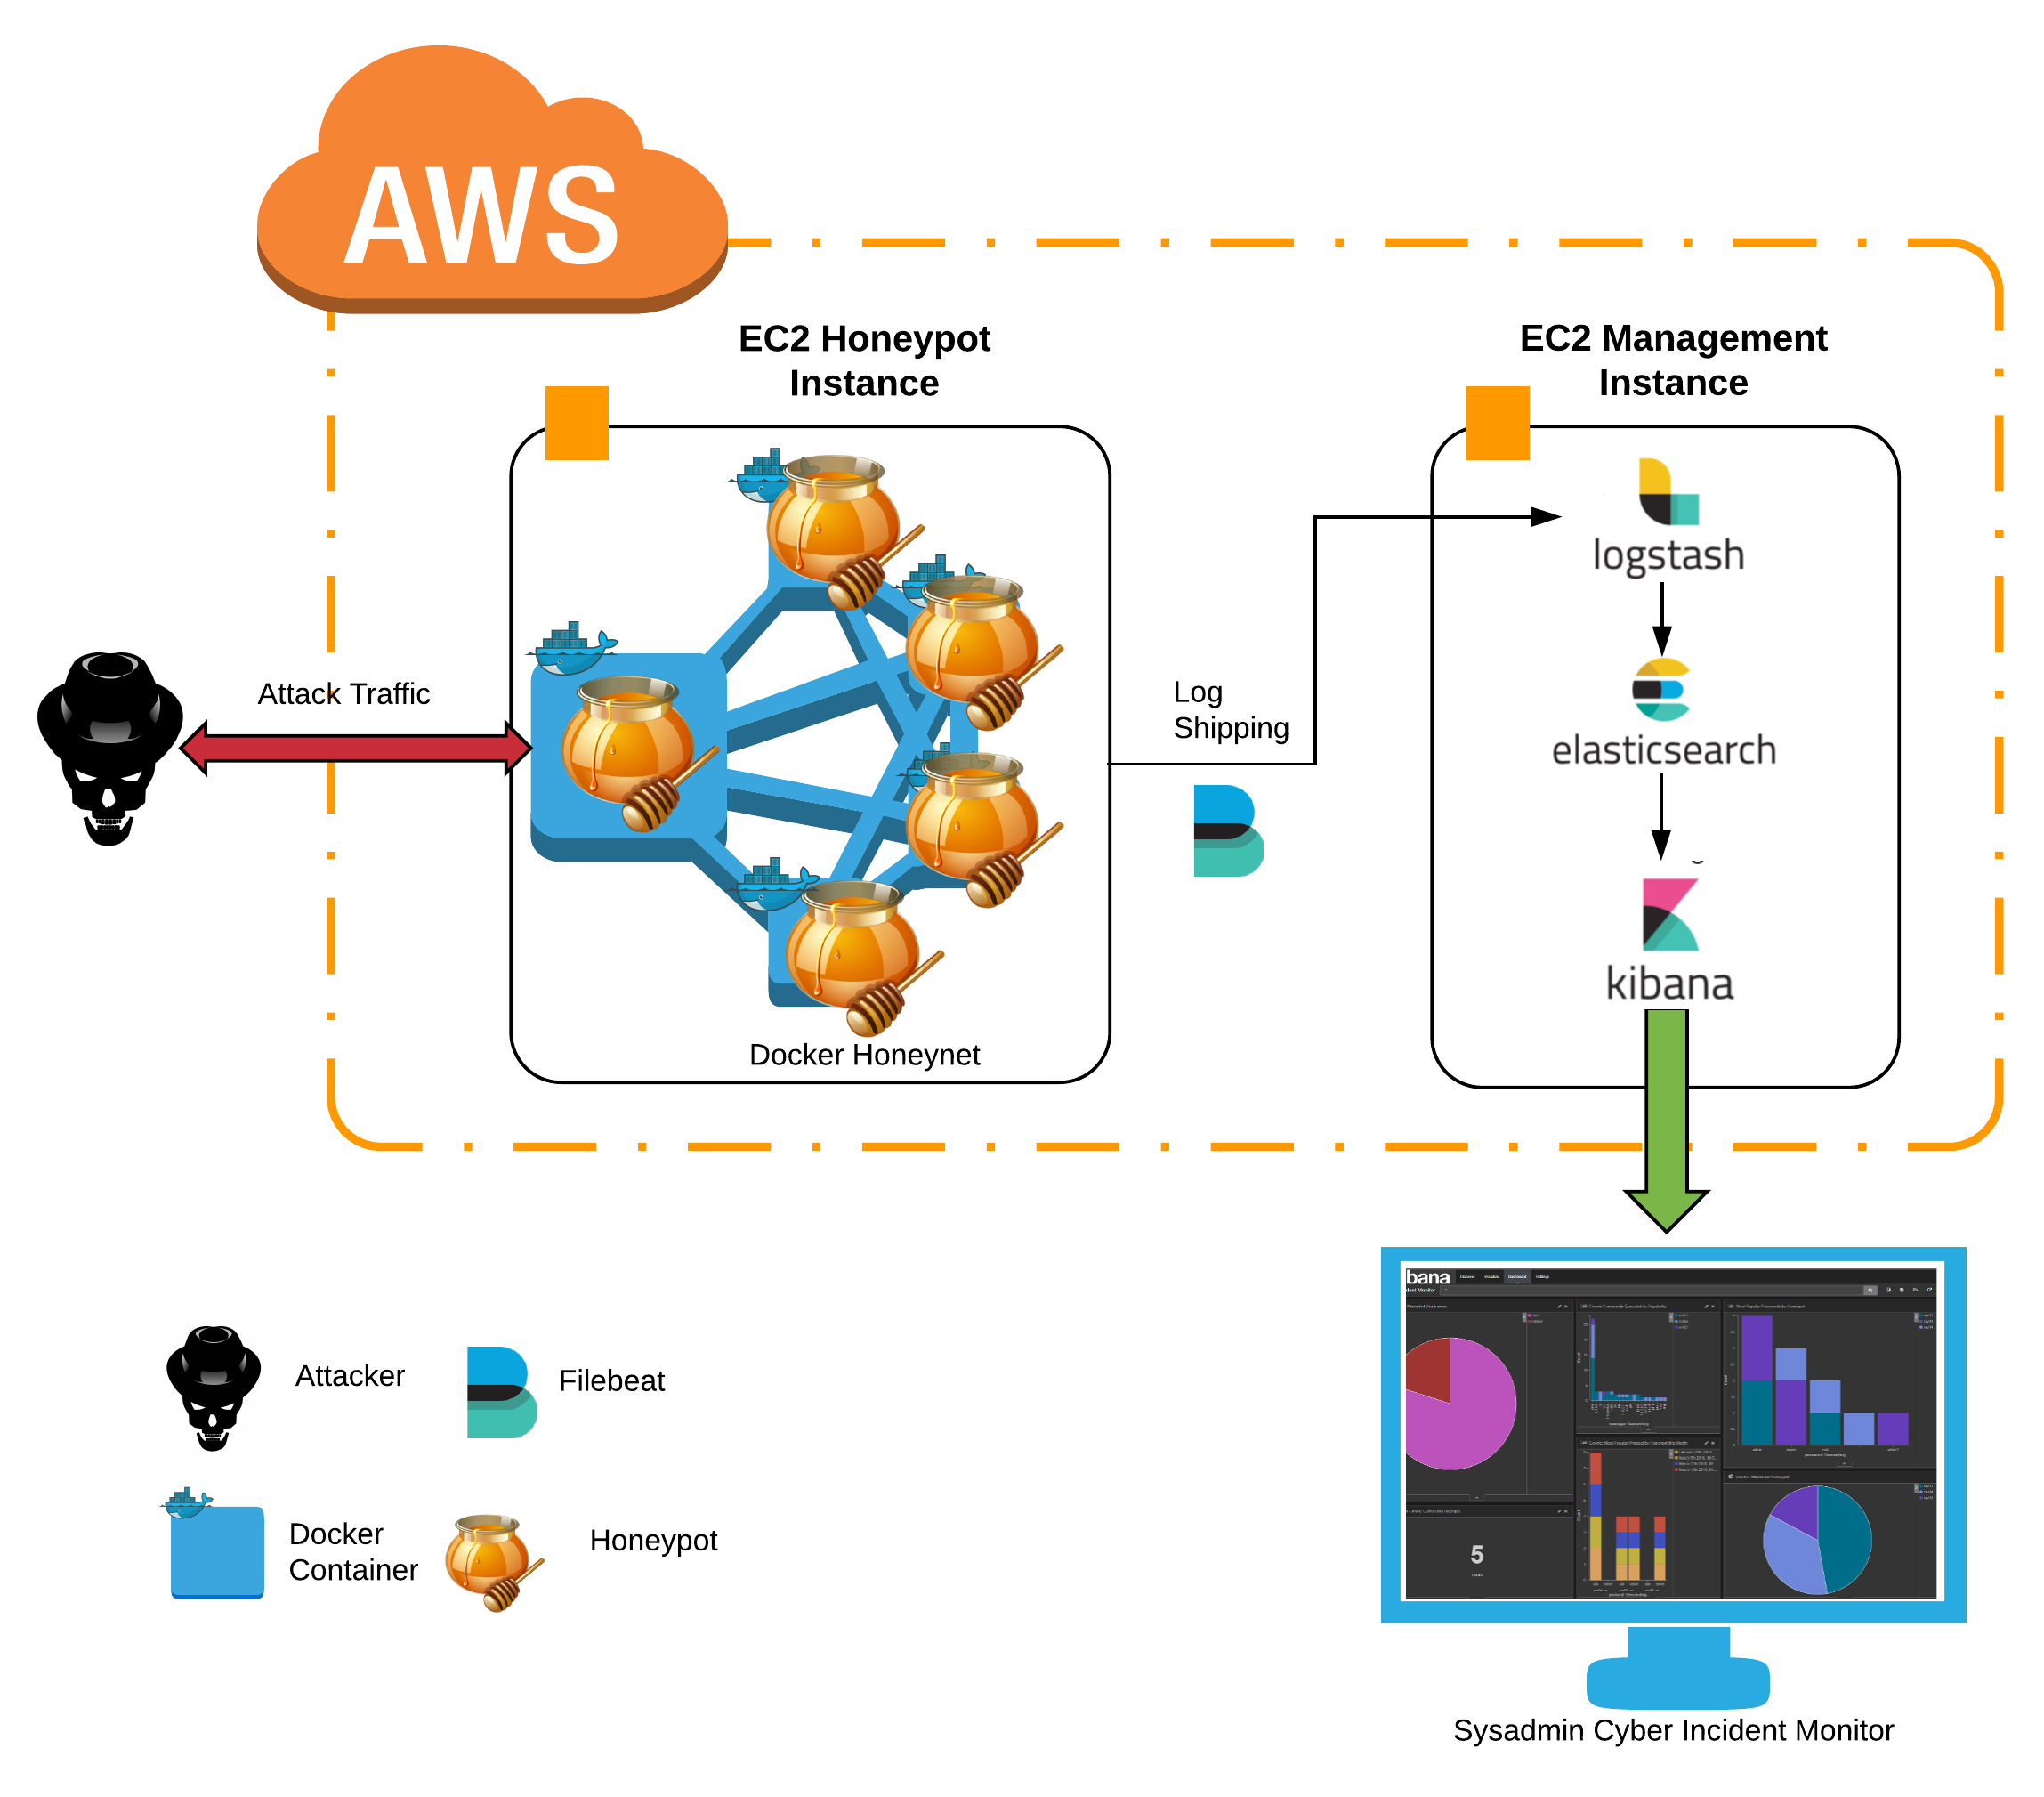
\includegraphics[width=160mm, scale=1]{Images/Cyber_Incident_Monitor_Architecture_Original_Design.png}
      \caption{Overview of the Proposed System Design} 
      \medskip
	  \small
		A high-level overview of the intended architecture and components of the system. The components include 2 AWS EC2 servers, a container network consisting of containerised honeypots hosted on the EC2 honeypot instance, an ELK log processing and visualisation pipeline hosted on the EC2 management instance, and a web console access to the visualisations generated by the system.
\label{fig:CyberIncidentMonitorSystemOriginalDesign}
\end{figure}

%\includewidefigure{CyberIncidentMonitorSystemOriginalDesign}{Overview of the Proposed System Design}{A high-level overview of the intended architecture and components of the system. The components include 2 AWS EC2 servers, a container network consisting of containerised honeypots hosted on the EC2 honeypot instance, an ELK log processing and visualisation pipeline hosted on the EC2 management instance, and a web console access to the visualisations generated by the system.}{Images/Cyber_Incident_Monitor_Architecture_Original_Design.png}

As part of a research progress update for this system 3 months after it had begun, a conceptual diagram similar to that provided in figure ~\ref{fig:CyberIncidentMonitorSystemOriginalDesign} was produced to give a high-level overview of the system architecture and operations. 


				%% DESIGN
\chapter{Implementation} \label{Chapter5}
In this chapter, the implementation of the various components of the research environment are described in-depth. This includes the challenges that were encountered in the implementation as well as alterations that were made to the system design as issues were unearthed.

In the interest of succinctness, low-level details of installation of tools etc. are not explained in great detail. Instead, attention in this section is given to the implementation of components of the system, detailing decisions that were made and the challenges that were faced in doing so.

\textit{Section \ref{UnderstandingContainerisedHoneypots}} describes an initial exploration of the major components that would be involved in the implementation of the proposed system: Namely AWS EC2, the Cowrie honeypot and Docker. The knowledge gained from this investigation is highlighted. 

\textit{Section \ref{HostServerSetup}} explains the process of deploying the AWS EC2 instances that would be used to host the research environment, and how they were configured to facilitate the requirements of the system.

\textit{Section \ref{BuildingTheDockerHoneynet}} details the configuration of the core component of the proposed system: The Docker honeynet. Details of the initial implementation of the containers and their inter-networking are described, before discussing a major challenge that was encountered in this process. A re-evaluated design and implementation is illustrated in detail, before finally explaining how the entire system was consolidated into a single deployable unit.

\textit{Section \ref{LoggingAndVisualisationSection}} explains the installation and configuration of the log processing and visualisation tools used, including how the honeypot data was provided to this system.

\textit{Section \ref{AlertSystemSection}} describes the configuration of PSAD, the alert generation system identified in the design phase as the tool of choice for notifying administrators of threats to their system.

Finally, \textit{Section \ref{ImplementationSummary}} provides a brief summary of what was achieved through the implementation of the system.



%% 
%% SECTION 1: Understanding Containerised Honeypots
%%

\section{Understanding Containerised Honeypots\label{UnderstandingContainerisedHoneypots}}
%Describing the initial setup that I had on the free tier instance, where I fiddled around with Cowrie and Docker.
In order to first understand the capabilities of AWS EC2, the Cowrie honeypot and Docker, some initial exploration of how these components work in practice formed a useful starting point. An AWS EC2 instance was first deployed, followed by a full installation of a Cowrie honeypot and finally some experimentation with Docker and its components.

\subsection{Deploying an AWS EC2 Instance} \label{DeployingAnAWSEC2Instance}
A single AWS EC2 instance was provisioned under the AWS 12-month free tier\footnote{The AWS free tier is an offer that allows certain AWS services to be used up to a limit for a defined period. For the EC2 service, the free-tier includes 750 hours of compute time on an EC2 server instance with 1 virtual CPU and 2GB of RAM for up to 12 months.} to facilitate exploring the Cowrie honeypot and the use of Docker containers.

\subsubsection{Provisioning an Instance}
Provisioning an EC2 instance on the free-tier is a straight-forward process, which involves creating an AWS account and following an EC2 deployment setup wizard, selecting the system specifications required. In this case, an Ubuntu 16.04 LTS server instance was provisioned with the same resource allocations as those provided with the free tier.

\subsubsection{Key Authentication}
As part of the deployment of an EC2 instance, an SSH public key\footnote{The encryption used by AWS for the generation of these keys is 2048-bit SSH-2 RSA encryption.} is generated. This key can then be used to securely authenticate with the instance over SSH  in place of password authentication. 

\subsubsection{Security Groups \label{AWSSecurityGroupsExploration}}
AWS EC2 uses \textit{security groups} to control the inbound and outbound traffic to an instance, and every EC2 instance must have at least one security group associated with it. Security groups act as a virtual firewall, with a set of security rules that define address ranges, protocols and ports that are permitted for communication with that instance. The default EC2 security group allows for SSH access over port 22/TCP from all IPv4 addresses. This default security group can be seen in figure \ref{fig:DefaultEC2SecurityRules}.

\begin{figure}[ht]
      \centering
      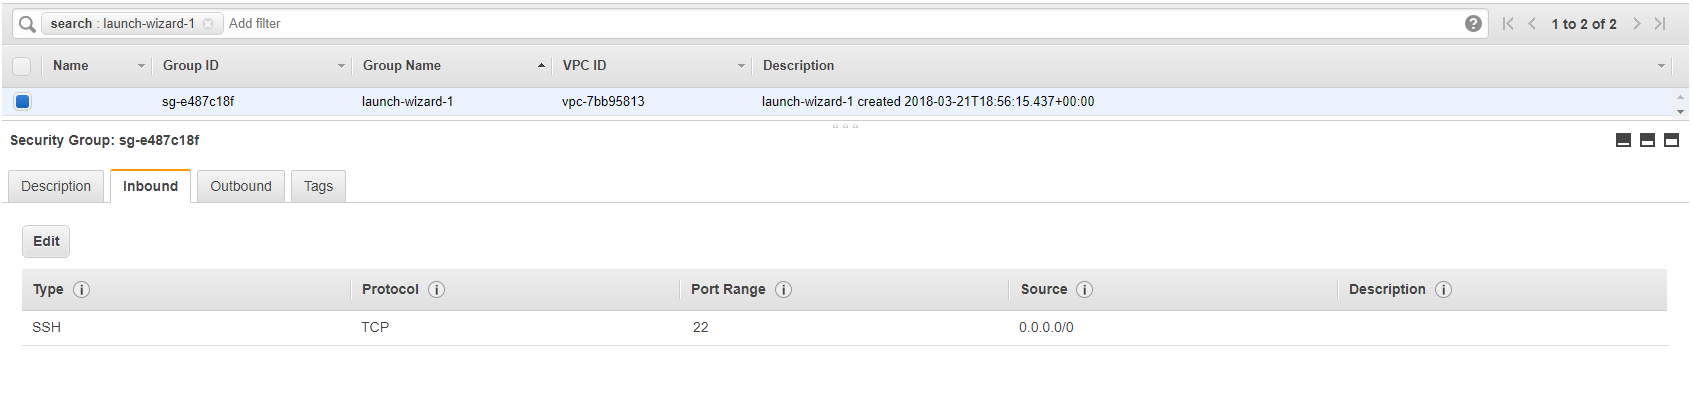
\includegraphics[width=160mm, scale=1]{Images/AWS_default_security_group_rules.PNG}
      \caption{AWS EC2 Default Security Rules} 
      \medskip
	  \small
		The default security group associated with an AWS EC2 instance when it is launched. The only security rule that is defined for this security group is SSH access over port 22/TCP from all IPv4 addresses.
\label{fig:DefaultEC2SecurityRules}
\end{figure}

%\includewidefigure{DefaultEC2SecurityRules}{AWS EC2 Default Security Rules}{The default security group associated with an AWS EC2 instance when it is launched. The only security rule that is defined for this security group is SSH access over port 22/TCP from all IPv4 addresses.}{Images/AWS_default_security_group_rules.PNG}
% TODO update with a snip


\subsection{The Cowrie Honeypot: A First Look}
By installing and configuring a plain Cowrie honeypot on the deployed AWS EC2 instance, it would be possible to understand the basic setup and configuration of the Cowrie honeypot before attempting to encapsulate it in a container environment. This was the next step undertaken in understanding the details of how the proposed system would be implemented.

\subsubsection{Installing Cowrie}    \label{InstallingCowrie}
As discussed in \textit{Section \ref{AboutCowrie}}, the Cowrie honeypot is an emulated of a Debian installation written in Python. A comprehensive installation guide for the Cowrie honeypot is provided on the Cowrie Github page. \cite{CowrieInstallationInstructions} By following this guide, it was relatively straight-forward to set up a Cowrie honeypot running as a Python \textit{virtualenv}\footnote{Python \textit{virtualenv} is a tool for creating isolated Python environments. It is used in Cowrie to create a virtual honeypot environment. \cite{VirtualEnvReference}}. The crucial requirement was to ensure that Cowrie is run by a non-root user, since it should be difficult for an attacker to achieve privilege escalation if they manage to interface directly with the host environment. Cowrie provides a safety net in this regard: If one was to attempt to launch the honeypot as a root user, it will fail to launch and output the log message \textit{'ERROR: You must not run cowrie as root!'}

The most significant configuration step in this process was to enable Cowrie to receive attack traffic destined for the EC2 host instance. By default, Cowrie listens for incoming traffic on ports 2222/TCP and 2223/TCP of its host, and thus for it to receive traffic from privileged ports 22/TCP (SSH) and 23/TCP (telnet)  some level of traffic forwarding was required. There are two approaches to achieving this recommended in the Cowrie installation guide: \cite{CowrieInstallationInstructions}

\begin{enumerate}
\item \textbf{Port Forwarding} 

Port forwarding involves using \textit{iptables} rules to forward incoming traffic on ports 22/TCP (SSH) and 23/TCP (telnet) to ports 2222/TCP and 2223/TCP.

\item \textbf{Direct Listening using Authbind}

As privileged ports, listening directly to incoming traffic on 22/TCP and 23/TCP requires root-user privileges. Cowrie will not run with such privileges, and so the \textit{authbind} Linux utility can be used to allow it to listen directly to traffic on these ports.

\end{enumerate}

In this initial installation of the Cowrie honeypot, listening as non-root using the \textit{authbind} utility was the approach taken.

The last step in this process is to update the configuration of the SSH daemon on the host instance so that it is still externally accessible by administrators. This is required since all incoming traffic on the default SSH port 22/TCP is now being forwarded to Cowrie, and involved a simple edit to the \textit{/etc/ssh/sshd\_config} file, changing the \textit{Port} value from 22/TCP to a different available port number. 



\subsubsection{Configuring Cowrie}
There are three primary components of Cowrie that can be used to customise the honeypot environment.
    \begin{itemize}
    \item \textit{\textbf{userdb.txt}}

    This file is used by Cowrie to determine what username-password combinations the honeypot should accept from an attacker. The default values for a clean Cowrie installation can be seen in figure \ref{fig:userdb_default}.
    
    \begin{figure}[ht]
      \centering
      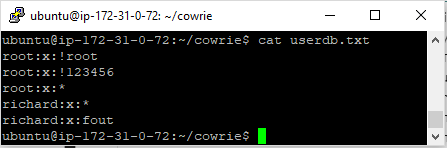
\includegraphics[width=160mm, scale=0.6]{Images/userdb_default_screenshot.PNG}
      \caption{Cowrie Honeypot Default Passwords} 
      \medskip
	  \small
		This image shows the default username-password combinations that are provided in Cowrie's \textit{userdb.txt} file. The first entry \textit{root:x:!root} specifies that username \textit{root} should be accepted, but not when the password specified is also \textit{root}. The third entry \textit{root:x:*} specifies that username \textit{root} should be accepted, with any other passwords for which there is no rule specified.
\label{fig:userdb_default}
\end{figure}
    
   % \includewidefigure{userdb_default}{Cowrie Honeypot Default Passwords}{This image shows the default username-password combinations that are provided in Cowrie's \textit{userdb.txt} file. The first entry \textit{root:x:!root} specifies that username \textit{root} should be accepted, but not when the password specified is also \textit{root}. The third entry \textit{root:x:*} specifies that username \textit{root} should be accepted, with any other passwords for which there is no rule specified.}{Images/userdb_default_screenshot.PNG}
    \item \textit{\textbf{cowrie.cfg}}

    This file is the main configuration file that is used by Cowrie to determine how to set up the honeypot environment. It comes with a multitude of settings, including parameters for integration with external tools\footnote{Currently, the external tool support for Cowrie listed on the Github repository README is listed as follows: Cuckoo Sandbox, ELK stack, Graylog, Kippo-Graph, Splunk, SQL (MySQL, SQLite3, RethinkDB). \cite{CowrieGithub}} and other parameters to control how the honeypot environment appears to an attacker. 
\item \textbf{honeyfs/}

It is possible to configure the file system contents of the honeypot environment through the addition of files and directories to the \textit{honeyfs/} directory. 
    \end{itemize}
    
    For this initial investigation into the operation of Cowrie, the configuration of all of  these components were left almost completely unaltered with default values.


\subsubsection{Exposing the Honeypot to Attacks}
\label{ExposingCowrieToAttack}
In order to understand the logging data produced by Cowrie, the honeypot was set up and exposed to the public internet. The installed Cowrie honeypot was configured with a name corresponding to a particular model of TPLink IP camera\footnote{The TPLink-TL-SC3171 model was chosen, since upon conducting a brief web search this model was immediately identified as having a Remote Code Execution (RCE) vulnerability: A highly desirable target. \cite{TPLinkIPCameraRCE}}, devices which are commonly targeted by IoT botnets. The default EC2 security group was left unaltered, meaning that the honeypot was exposed to the entire IPv4 address space on port 22/TCP (SSH). 

The environment was exposed for 1 hour, and in that time logged brute-force authentication attacks from 4 different IP addresses. These attacks were identified to be  bot attacks\footnote{Based on the timestamps logged by Cowrie, subsequent login attempts were spaced broadly 1 second apart: A speed which would be difficult for a human attacker to achieve consistently, leading to the classification of these attacks as bot attacks.} whose source IP addresses were identified to be from multiple different countries including Egypt, Russia, China and Vietnam\footnote{The source location was determined by using \textit{Maxmind GeoIP Database} which approximates the geolocation of IP addresses. \cite{MaxmindGeoipDatabase}}. 

One of the attack sessions was of particular interest, since upon comparison of the attempted login credentials it was observed that several of the passwords were the same as those identified by Antonakakis \textit{et al.} in the source code of the Mirai botnet\footnote{A number of the default passwords observed by Antonakakis \textit{et al.} in their research can be seen in \textit{Section \ref{IoTBotnetsSoA}}. Of these, passwords \textit{admin}, \textit{7ujMko0admin}, \textit{1234}, \textit{admin1234}, \textit{default}, \textit{password} were passwords in common with the bot attack observed here. The highly unusual password \textit{7ujMko0admin} would appear to indicate that this attack was conducted by a device that had been compromised by Mirai or one of its variants.}. \cite{UnderstandingTheMiraiBotnet} This was an interesting find, and illustrates the sheer scale of the infection of devices by this botnet and its variants.

The Cowrie log, which captured the attack session data in JSON format, gave an insight into the level of detail of information that Cowrie can capture. The information captured in these sessions included:

\begin{itemize}
\item The source IP and port of the connection;
\item The remote SSH protocol version and encryption algorithm used;
\item The username-password combinations that were attempted, and whether the attempt succeeded or failed;
\item How long the connection was maintained for, and the reason why the connection was terminated\footnote{For example, this could be something like too many incorrect login attempts, in which case the message ''too many bad auths'' would be logged by Cowrie.};
\item Timestamps corresponding to each event, and a unique session ID per connection.
\end{itemize}

As information that would later be processed by the ELK stack tools in the incident monitoring system, seeing the level of detail of JSON logging provided by Cowrie was useful towards understanding what visual data could potentially be generated from honeypot logs.

%
%	Building Docker Containers (Experimentation)
%

\subsection{Building Docker Containers}
The Docker ecosystem is straight-forward in principle, but is composed of a number of distinct components that together enable the stateless hosting of applications in containers. Understanding the components of this ecosystem and how they interoperate would be essential to effectively using this technology to implement the honeynet.

The basic Docker-Cowrie source code provided by the Cowrie Project \cite{DockerCowrie} was used to understand the construction of container environments and how to interoperate them before progressing to the implementation of the containerised honeynet.

\subsubsection{Docker Images}
A Docker container environment is completely specified by its image definition. This image definition can be defined using a \textit{Dockerfile}. The Dockerfile defines what the environment inside a container looks like, and consists of a set of text commands that are used to build the image\footnote{The full set of commands that can be specified in a Dockerfile can be found in the Docker documentation. \cite{AllCommandsForDockerfiles}}. Any external files referred to within the Dockerfile form part of the \textit{build context} of the image.

The lifecycle of a container is often referred to as the \textit{build-and-run} cycle, illustrated in figure \ref{fig:DockerBuildAndRun}\footnote{This illustration is adapted from a diagram in a presentation given by the authors of the paper \textit{Using Docker Containers to Improve Reproducibility in Software and Web Engineering Research.} \cite{ReproducableResearchEnvironmentsContainers} \cite{DockerBuildAndRunDiagram}.}.

\begin{enumerate}
\item \textbf{Building a Docker Image}

By issuing the \textit{docker build} CLI command with reference to a Dockerfile, a container image is generated by the Docker engine using the Dockerfile and the build context. The instructions in the Dockerfile are executed one-by-one and committed incrementally to the new image before finally generating an ID for the image. The new image usually uses a \textit{base image} as a foundation, which is a top-level image upon which other images can be built.

\item \textbf{Running a Docker Container}

If the \textit{docker create [arguments] [image-ID]} CLI command is issued with reference to an image ID, a writeable container layer is created based on that image and is prepared for running using any arguments provided. The resulting container layer is tagged with a container ID. However, the container is not automatically launched after being created: Issuing a \textit{docker start [container-ID]} CLI command will launch the container.

If instead the \textit{docker run [arguments] [image-ID]} command is issued with reference to the image ID, the same writeable container layer is created and the container is immediately launched. 

\item \textbf{Stopping or Removing a Container}

After being launched, a container can be stopped using the \textit{docker stop [container-ID]} command. The container can also be removed using the \textit{docker container rm [container-ID]} command, but only if either (i) it is not running, or (ii) it is running but the removal is forced by specifying additional arguments.

\end{enumerate}

    \begin{figure}[ht]
      \centering
      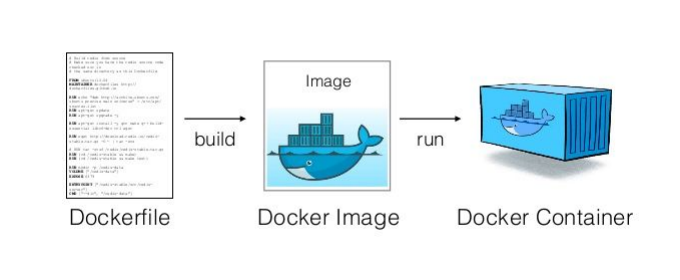
\includegraphics[width=160mm, scale=1]{Images/Docker_build_and_run_cycle.png}
      \caption{The Docker \textit{build-and-run} Cycle} 
      \medskip
	  \small
		An adapted illustration of the Docker \textit{build-and-run} cycle. The Dockerfile is used to build a Docker image, which in turn is used to run a Docker container.
\label{fig:DockerBuildAndRun}
\end{figure}

%\includewidefigure{DockerBuildAndRun}{The Docker \textit{build-and-run} Cycle}{An adapted illustration of the Docker \textit{build-and-run} cycle. The Dockerfile is used to build a Docker image, which in turn is used to run a Docker container.}{Images/Docker_build_and_run_cycle.png}


\subsubsection{Entrypoint Scripts}
Different elements of a container environment must be configured at particular points in the container lifecycle: Certain configuration options can be specified pre-runtime, whilst others must be specified at runtime. For example, one cannot update a container's internal routing table until that container is actually running, and hence this configuration cannot be directly specified as part of the static Docker image. This seems a nuisance since it means that not all environment configuration can be directly defined within the container image, but it is here that the use of the Docker \textit{ENTRYPOINT} command becomes useful.

The \textit{ENTRYPOINT} command can be used in a Dockerfile to specify a script which should be run when a container using that image is launched. This means that in the previous example, a script defining updates to the container's internal routing table can be specified as the \textit{ENTRYPOINT} command in the Dockerfile. After launching the container, this script will be executed and the routing table will be updated. This is a useful and flexible option in the configuration of a container environment.

%- Needed to be able to allow non-root container user to write to a docker volume directory.

\subsubsection{Docker Volumes} \label{DockerVolumesExperimentation}
Docker volumes were discussed in \textit{Section \ref{PersistingDockerContent}} as a means of persisting volatile content generated by a container. They can be mounted by using the \textit{VOLUME} command in the Dockerfile for a container image, and the corresponding host directory to which they are mapped is specified as an argument to the \textit{docker create} or \textit{docker run} CLI commands at a later stage. Once a container is stopped, any volumes that are mounted to it and their contents are persisted: It is only when the container is completely removed that the volume is also removed.

Figure \ref{fig:DockerVolumes} shows a conceptual view of how volumes can be used to persist content generated within a container, on the host system. 

    \begin{figure}[ht]
      \centering
      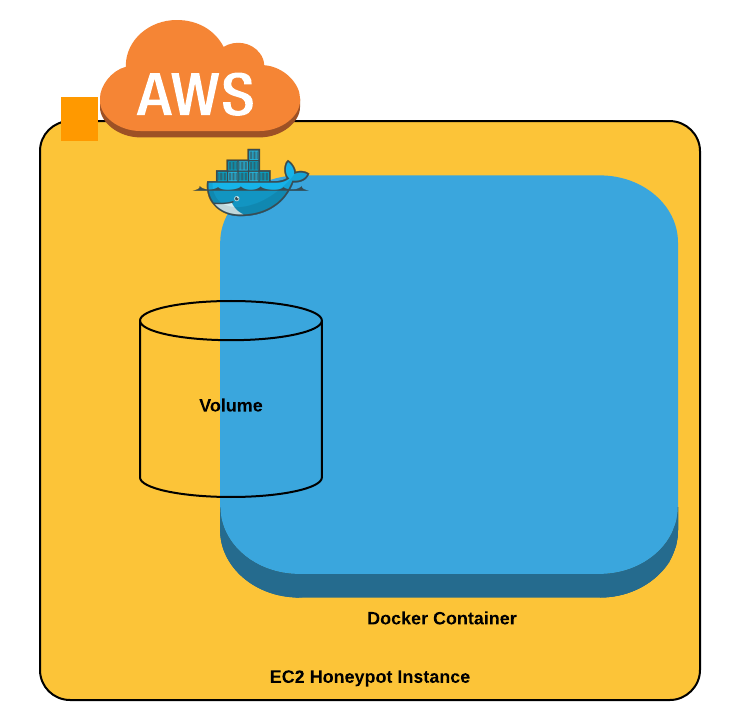
\includegraphics[width=125mm, scale=1]{Images/Another_illustration_of_how_a_Docker_volume_looks.png}
      \caption{A Conceptual Representation of Docker Volumes} 
      \medskip
	  \small
		A conceptual view of how Docker volumes operate. Files in this volume are accessible both from the host and the container in a specific directory on each system. Changes can be made dynamically to the contents of either directory and are immediately available in the corresponding mapped directory. 
\label{fig:DockerVolumes}
\end{figure}

%\includewidefigure{DockerVolumes}{A Conceptual Representation of Docker Volumes}{A conceptual view of how Docker volumes operate. Files in this volume are accessible both from the host and the container in a specific directory on each system. Changes can be made dynamically to the contents of either directory and are immediately available in the corresponding mapped directory. }{Images/Another_illustration_of_how_a_Docker_volume_looks.png}


\subsubsection{Docker Networking}
    Containers, like a physical machine, have their own networking stack. Each container has its own ports, and can have virtual interfaces connecting them to virtual Docker networks. This is the key piece of functionality that makes Docker so well-suited to the implementation of the honeynet in the proposed system.
    
    There are two different ways of exposing ports through the \textit{docker create} and \textit{docker run} CLI commands, which have different effects. 
\begin{itemize}

\item Using the \textit{--expose} argument exposes the specified container port to the host machine and to other containers. It is not however published to the host's network interfaces.

\item On the other hand, using the \textit{--publish} argument publishes the specified container port to the host's network interfaces meaning that it is accessible through these ports on the public internet.
\end{itemize}

An \textit{EXPOSE} argument can also be specified in the Dockerfile of an image, meaning that when a container is built from that image the specified ports are exposed for \textit{inter-container communication} only.  This is the default option specified in the Docker-Cowrie Dockerfile built by the Cowrie Project developers. \cite{DockerCowrie}

All containers, unless a network is otherwise specified, are automatically connected to a default Docker bridge network\footnote{As explained in the Docker documentation, \cite{UseBridgeNetworksDocker} ''a bridge network is a Link Layer device which forwards traffic between network segments... In terms of Docker, a bridge network uses a software bridge which allows containers connected to the same bridge network to communicate.''} called \textit{bridge} once created. This network allows the containers to communicate directly with each other and with the host machine through a virtual network interface called \textit{docker0}. Additional networks can be manually defined as bridge or overlay\footnote{An overlay network is described in the Docker documentation as ''a distributed network among multiple Docker daemon hosts. This network sits on top of (overlays) the host-specific networks, allowing containers connected to it ... to communicate securely. \cite{UseOverlayNetworksDocker} } networks. 

\subsection{Conclusions} \label{ConclusionsToExperimentationSection}
%Anything in relation to the use of these tools together.
Having explored the operation of AWS EC2, the Cowrie honeypot and the Docker container ecosystem, a solid understanding and some basic configuration had been achieved regarding the next steps in the implementation of the research environment described in \textit{Chapter 4}.  In particular, by the time all of the aforementioned Docker functionalities had been explored a rudimentary deployment script named \textit{do\_honeypot.sh} had been developed for the rapid removal and deployment of containers. This script could, based on simple parameters, perform functions including:

\begin{itemize}
\item Building the basic Docker-Cowrie image;
\item Creating a container based on the pre-built image, given a unique container name;
\item Launching and stopping a container given its name;
\item Entering a running container, presenting an internal container CLI to the user;
\item Providing usage instructions on how to use the script to manage containers on the system.
\end{itemize}

This, coupled with the knowledge gained about the operation of Cowrie and AWS EC2, formed a solid starting point from which to begin implementing the research environment.



%% 
%% SECTION 2: Host Server Setup
%%


\section{Host Server Deployment} \label{HostServerSetup}

There were two AWS EC2 server instances deployed for the implementation of the system: A honeypot server instance and a management server instance, as designed in \textit{Chapter 4}. The same deployment process described in \textit{Section \ref{DeployingAnAWSEC2Instance}} was followed. Both instances were hosted in the Amazon US East (Ohio) availability zone\footnote{As explained in the AWS EC2 documentation, ''Amazon EC2 is hosted in multiple locations world-wide. These locations are composed of regions and Availability Zones. Each region is a separate geographic area. Each region has multiple, isolated locations known as Availability Zones.'' \cite{WhatAreAWSAvailabilityZones}} running Ubuntu 16.04 LTS operating systems. Each instance was allocated different hardware resources depending on their requirements. In both cases, the hardware requirements were such that those provided by the AWS 12-month free tier were not sufficient, meaning that more expensive cost-incurring instances were needed.

\subsection{The EC2 Honeypot Server Instance}
	
	In order to host a number of Docker containers as part of the proposed containerised honeynet, a relatively powerful server instance was required. Based on the initial experimentation with running Docker containers on the free-tier instance, an EC2 instance with 16GB RAM and 4 virtual CPUs was provisioned in order to allow multiple Docker containers to be hosted\footnote{The free-tier specifications of 2GB RAM were determined to be insufficient for hosting multiple Docker containers, since it was found that multiple Docker containers launched simultaneously would cease to run due to memory shortages.}. 
	
    To be able to attract the attention of IoT bots scanning the public internet for vulnerable devices, the SSH (22/TCP) and telnet (23/TCP) default ports needed to be visible on this server instance. In total, just these two ports were exposed to the entire public internet by configuring security rules\footnote{It was deemed unnecessary to allow access on other ports, since for the purpose of collecting data for experiments the activities of interest were limited to attacks over SSH and telnet as are typical of IoT botnets.}\textsuperscript{,}\footnote{During the initial development of the system, access to these two ports was restricted through the AWS EC2 security rules to a select IP address for testing purposes.}. 
    
    One other port was opened on the server instance but with greater access restrictions. As described in \textit{Section \ref{InstallingCowrie}}, the purpose of this port is to ensure that administrative access to this server instance would be maintained. The port was chosen at random as 45678/TCP, and was exposed only to the IP address of the management instance to obscure the fact that this port was open as much as possible.
    
All security rules configured for the honeypot server instance can be seen in figure \ref{fig:HoneypotInstanceSecurityRules}.

    \begin{figure}[ht]
      \centering
      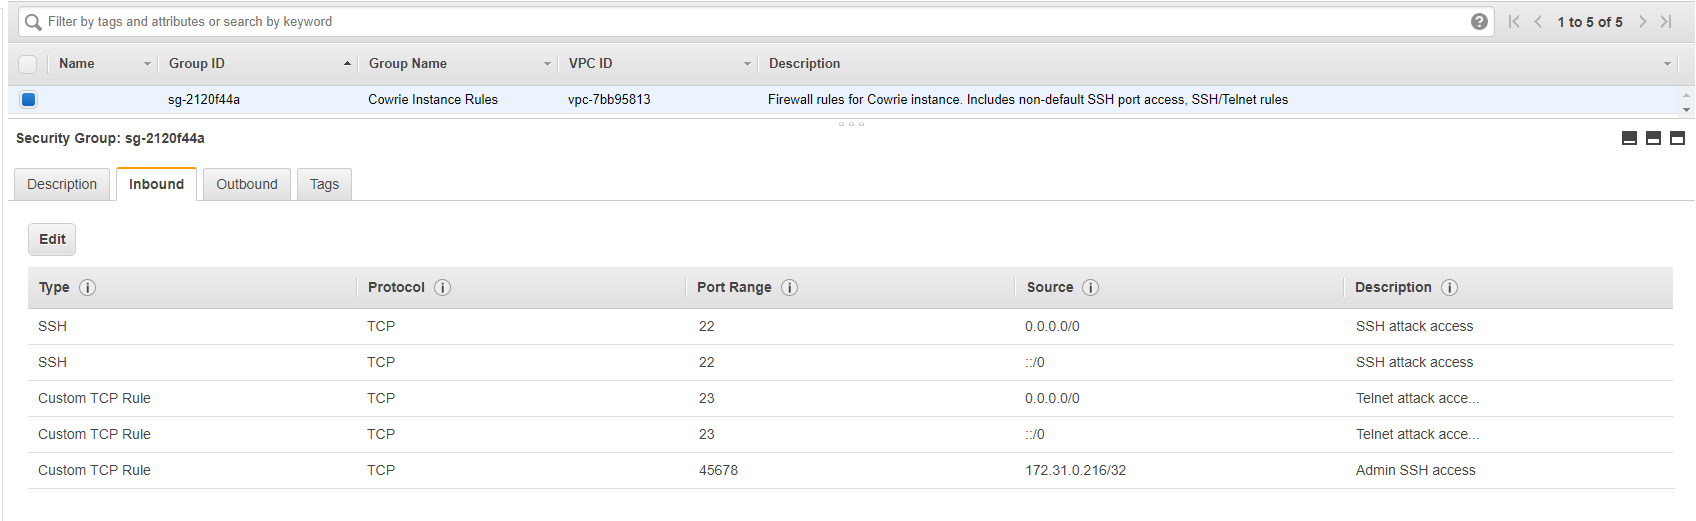
\includegraphics[width=160mm, scale=1]{Images/AWS_honeypot_instance_security_group_rules.PNG}
      \caption{AWS EC2 Honeypot Server Instance Security Rules} 
      \medskip
	  \small
		The 'Cowrie Instance Rules' security group, showing the rules defined for access to the AWS EC2 honeypot server instance. For each of SSH (22/TCP) and telnet (23/TCP), these ports were exposed to the entire IPv4 and IPv6 address spaces, whilst port 45678/TCP was only exposed to the IP address of the management server instance.
\label{fig:HoneypotInstanceSecurityRules}
\end{figure}

%\includewidefigure{HoneypotInstanceSecurityRules}{AWS EC2 Honeypot Server Instance Security Rules}{The 'Cowrie Instance Rules' security group, showing the rules defined for access to the AWS EC2 honeypot server instance. For each of SSH (22/TCP) and telnet (23/TCP), these ports were exposed to the entire IPv4 and IPv6 address spaces, whilst port 45678/TCP was only exposed to the IP address of the management server instance.}{Images/AWS_honeypot_instance_security_group_rules.PNG}
	
    
\subsection{The EC2 Management Server Instance} \label{DeployingTheManagementInstance}
    
	Since the management server instance was required to host the ELK log processing stack, there were certain minimum hardware resources required to be able to run these tools. Due to cost considerations, a minimal set of resources were allocated to meet the requirements: A server with 4GB of RAM and 2 virtual CPUs\footnote{The default RAM allocated to Elasticsearch, which is more resource-hungry than Logstash and Kibana, is 1GB. \cite{ElasticsearchHeapSizing} Upon the first installation of Elasticsearch on a server with 2GB RAM, it was found that this memory allocation was insufficient since Elasticsearch would continuously run out of heap memory. In a comprehensive tutorial by DigitalOcean which explains the steps required to configure these tools on an Ubuntu installation, 4GB of RAM was deemed sufficient. \cite{DigitalOceanELKTutorial} This led to the eventual decision to allocate a server with 4GB of RAM.} . The installation and configuration of the tools to be hosted on this EC2 instance are described later in \textit{Section \ref{LoggingAndVisualisationSection}}.

On this server instance, there were three ports which were exposed using security rules:
	\begin{itemize}
    	\item Port 22/TCP for SSH administrator access;
        \item Port 5045/TCP, which was a port randomly chosen to allow the honeypot server instance to transfer logs to the management server instance;
        \item Port 80/TCP, to allow HTTP access from a web browser to view the visualisations that would later be available from this server.
	\end{itemize}
    
 All security rules configured for the management server instance can be seen in figure \ref{fig:ManagementInstanceSecurityRules}.

 \begin{figure}[ht]
      \centering
      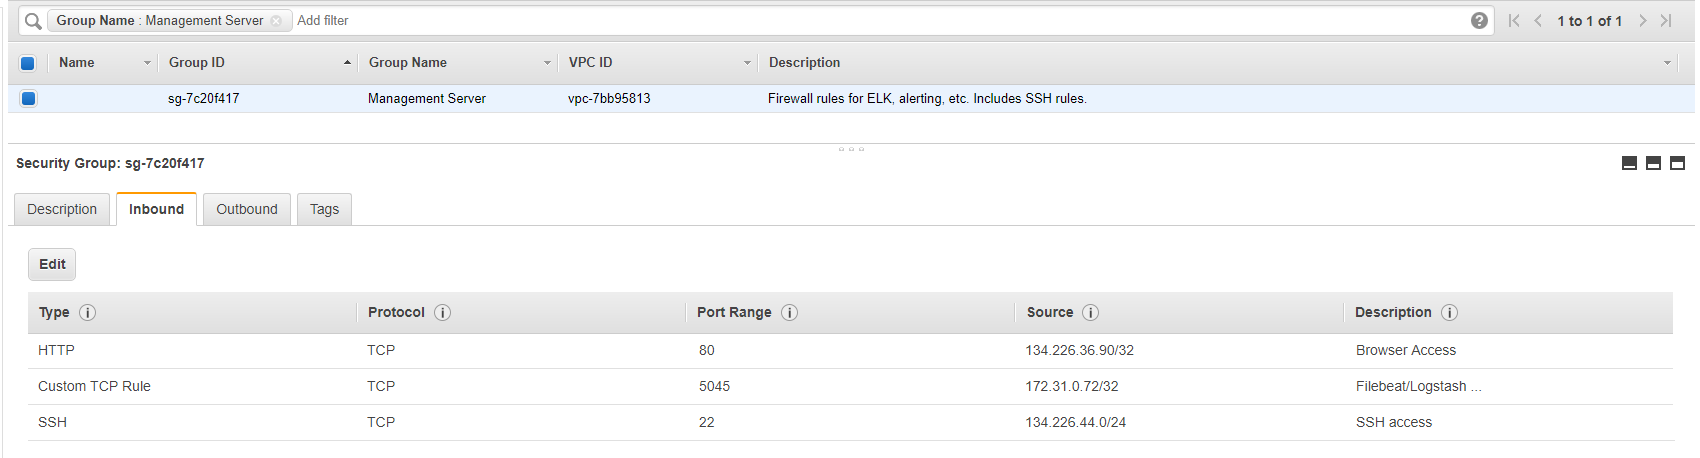
\includegraphics[width=160mm, scale=1]{Images/AWS_management_instance_security_group_rules.PNG}
      \caption{AWS EC2 Management Server Instance Security Rules} 
      \medskip
      \small
		The 'Management Server' security group, showing the rules defined for access to the AWS EC2 management server instance. Port 80/TCP here is seen to be exposed to a single IP address, from which access to the visualisations generated could be accessed via a web session. Port 5045/TCP is exposed to the IP address of the honeypot server instance to allow the Filebeat log-shipping application to transfer encrypted log files to the management server instance. Port 22/TCP is also exposed to a single IP address to allow administrative access to the instance.
\label{fig:ManagementInstanceSecurityRules}
\end{figure}

%\includewidefigure{ManagementInstanceSecurityRules}{AWS EC2 Management Server Instance Security Rules}{The 'Management Server' security group, showing the rules defined for access to the AWS EC2 management server instance. Port 80/TCP here is seen to be exposed to a single IP address, from which access to the visualisations generated could be accessed via a web session. Port 5045/TCP is exposed to the IP address of the honeypot server instance to allow the Filebeat log-shipping application to transfer encrypted log files to the management server instance. Port 22/TCP is also exposed to a single IP address to allow administrative access to the instance.}{Images/AWS_management_instance_security_group_rules.PNG}




%% 
%% SECTION 3: The Docker Honeynet
%%


\section{Building the Docker Honeynet\label{BuildingTheDockerHoneynet}}
One of the initial considerations that was described in \textit{Section \ref{EaseOfDeploymentDesignDecision}} was that the Docker honeynet should be deployable automatically by recording all commands required to build the networked environment in bash scripts. Throughout the development of the Docker honeynet described in this section, the \textit{do\_honeypot.sh} deployment script described in \textit{Section \ref{ConclusionsToExperimentationSection}} was incrementally expanded to include multiple functions and verbose output messages for easy deployment, removal and maintenance of the honeynet.

%
% COWRIE CONTAINER    
%
\subsection{The Cowrie Container}
It was decided in the design phase that the Docker image for the Cowrie honeypot containers would be heavily based off the existing image developed by the maintainers of the Cowrie Project, which had already been explored in the experimentation phase. \cite{DockerCowrie} This image definition provides a sound basis for building an enhanced Cowrie container image which can facilitate the inter-networking of multiple containers in a honeynet configuration.


\subsubsection{Building an Enhanced Docker Image}
The Dockerfile developed by the maintainers of the Cowrie Project performs the following operations when being built into an image:

\begin{itemize}
\item The \textit{debian:jessie-slim} base OS image is downloaded and used as a foundation for the container image.
\item All dependencies required by Cowrie are installed, most of which are build dependencies.
\item The Cowrie application is configured in accordance with the mandatory installation steps specified on the Cowrie Github repository, \cite{CowrieInstallationInstructions} before removing all unnecessary build packages.
\item A non-root user \textit{cowrie} is created, and set as the default user for the container.
\end{itemize}

The Dockerfile also specifies a command to launch Cowrie at runtime under the \textit{cowrie} user, as well as specifying a working directory \textit{/cowrie/cowrie-git/}, mounting two Docker volumes and exposing ports 2222/TCP and 2223/TCP, the default host ports on which Cowrie listens for incoming traffic. 

The creation of a default non-root user and removal of unnecessary build packages make the container environment suitably restrictive in the event that an attacker was able to bypass the Cowrie application and interface directly with the underlying container. Additional customisations were added to this base image definition to facilitate functions required by the Cowrie honeynet.

\subsubsection{Additional Linux Utilities}
The Cowrie application is capable of emulating many common Linux utilities including \textit{cat}, \textit{wget}, \textit{echo} and many others. As an open-source project it is even possible to add new utility emulations if desired. Thus, there are very few packages that actually need to be installed on the Cowrie container, and those that are required are mostly build dependencies. \cite{DockerCowrie} The only additional dependency required was \textit{authbind}, to allow Cowrie to receive incoming attack traffic from its host container. 

In the customised Cowrie Dockerfile, an \textit{entrypoint script} was specified to be executed at container runtime. This script was used to configure \textit{authbind} as in \textit{Section \ref{InstallingCowrie}} so that Cowrie could listen to traffic on ports 22/TCP (SSH) and 23/TCP (telnet) of the container. The script is shown in Snippet 5.1. \mbox{}\\ 
\mbox{}\\
\mbox{}
\linebreak

\includecode{Cowrie entrypoint script}{The entrypoint script specified in the customised Cowrie Dockerfile. This shows the configuration of \textit{authbind} by creating 2 new empty files using \textit{touch}, the assignment of ownership of these files to the \textit{cowrie} user, and full read-write-execute permissions being given to \textit{cowrie} user for both of these files. This allows the \textit{cowrie} user to use \textit{authbind} to receive incoming traffic on these ports. Cowrie then needs to be notified that \textit{authbind} is being used, achieved by setting the \textit{AUTHBIND\_ENABLED} configuration parameter. Finally, the script launches the Cowrie honeypot under the \textit{cowrie} user.}{Code_snippets/cowrie_listen_authbind.sh}\label{cowrie_entrypoint_script}


\subsubsection{Sharing and Persisting Container Data}
As identified in \textit{Section \ref{PersistingDockerContent}} and explored in \textit{Section \ref{DockerVolumesExperimentation}}, volumes are useful for dynamically sharing information between a container and its host. The use of volumes in the Cowrie containers in this system serves two purposes:

\begin{enumerate}
\item Cowrie configuration files can be specified on the host, and accessed by a container through a shared volume;
\item Logs generated inside a container by Cowrie can be accessed by the host through a shared volume, making them both accessible and persistent outside the container.
\end{enumerate}

Thus, in the honeynet deployment script an extended function was defined for the creation of Cowrie containers, specifying a number of volumes to be mounted to them.

\begin{itemize}
\item The \textit{dl/} directory in the Cowrie container was mounted as a volume to allow container access from the host. This is the default location where checksums of attempted downloads by attackers are stored.
\item The \textit{log/} directory in the Cowrie container was mounted as a volume to allow container access from the host. This is the default location where log files generated by Cowrie are stored.
\item The \textit{data/} directory in the Cowrie container was also mounted as a volume to allow host access from the container. This is the default location for the \textit{userdb.txt} password configuration file used by Cowrie.
\end{itemize}

As well as using volumes to make configuration files available inside Cowrie containers, the \textit{docker cp} command was used to copy the \textit{cowrie.cfg} file from the host into the container without using a volume\footnote{This was necessary because of an intricacy in the mounting of nested volumes from the host to a container: If the directory containing this file was mounted as a volume to the container, an issue would arise where the volumes corresponding to the nested \textit{/data}, \textit{/log} and \textit{/dl} directories would be overwritten.}. 


\subsubsection{Port Publication}
Because all containers need to be able to communicate with each other over ports 22/TCP and 23/TCP to enable the desired attack propagation between honeypots in the honeynet, the \textit{EXPOSE} command was used in the Cowrie Dockerfile. This meant that when launched, ports 22/TCP and 23/TCP on any Cowrie container would be visible to any other containers on the default Docker \textit{bridge} network.

In the case of the honeywall Cowrie container, the situation was slightly different: In order to be able to receive attacks, it needed to be able to access incoming traffic from the network interface of the host. To achieve this, when creating the honeywall container the \textit{--publish} argument was used to map ports 22/TCP and 23/TCP on the host network interface to the corresponding ports on the container. The use of the \textit{--publish} argument also meant that the container would automatically be assigned a virtual network interface on the \textit{bridge} Docker network, such that it would be able to receive the incoming network traffic on these ports from the host instance. Figure \ref{fig:HoneywallPortPublication} illustrates how this looks conceptually.

 \begin{figure}[ht]
      \centering
      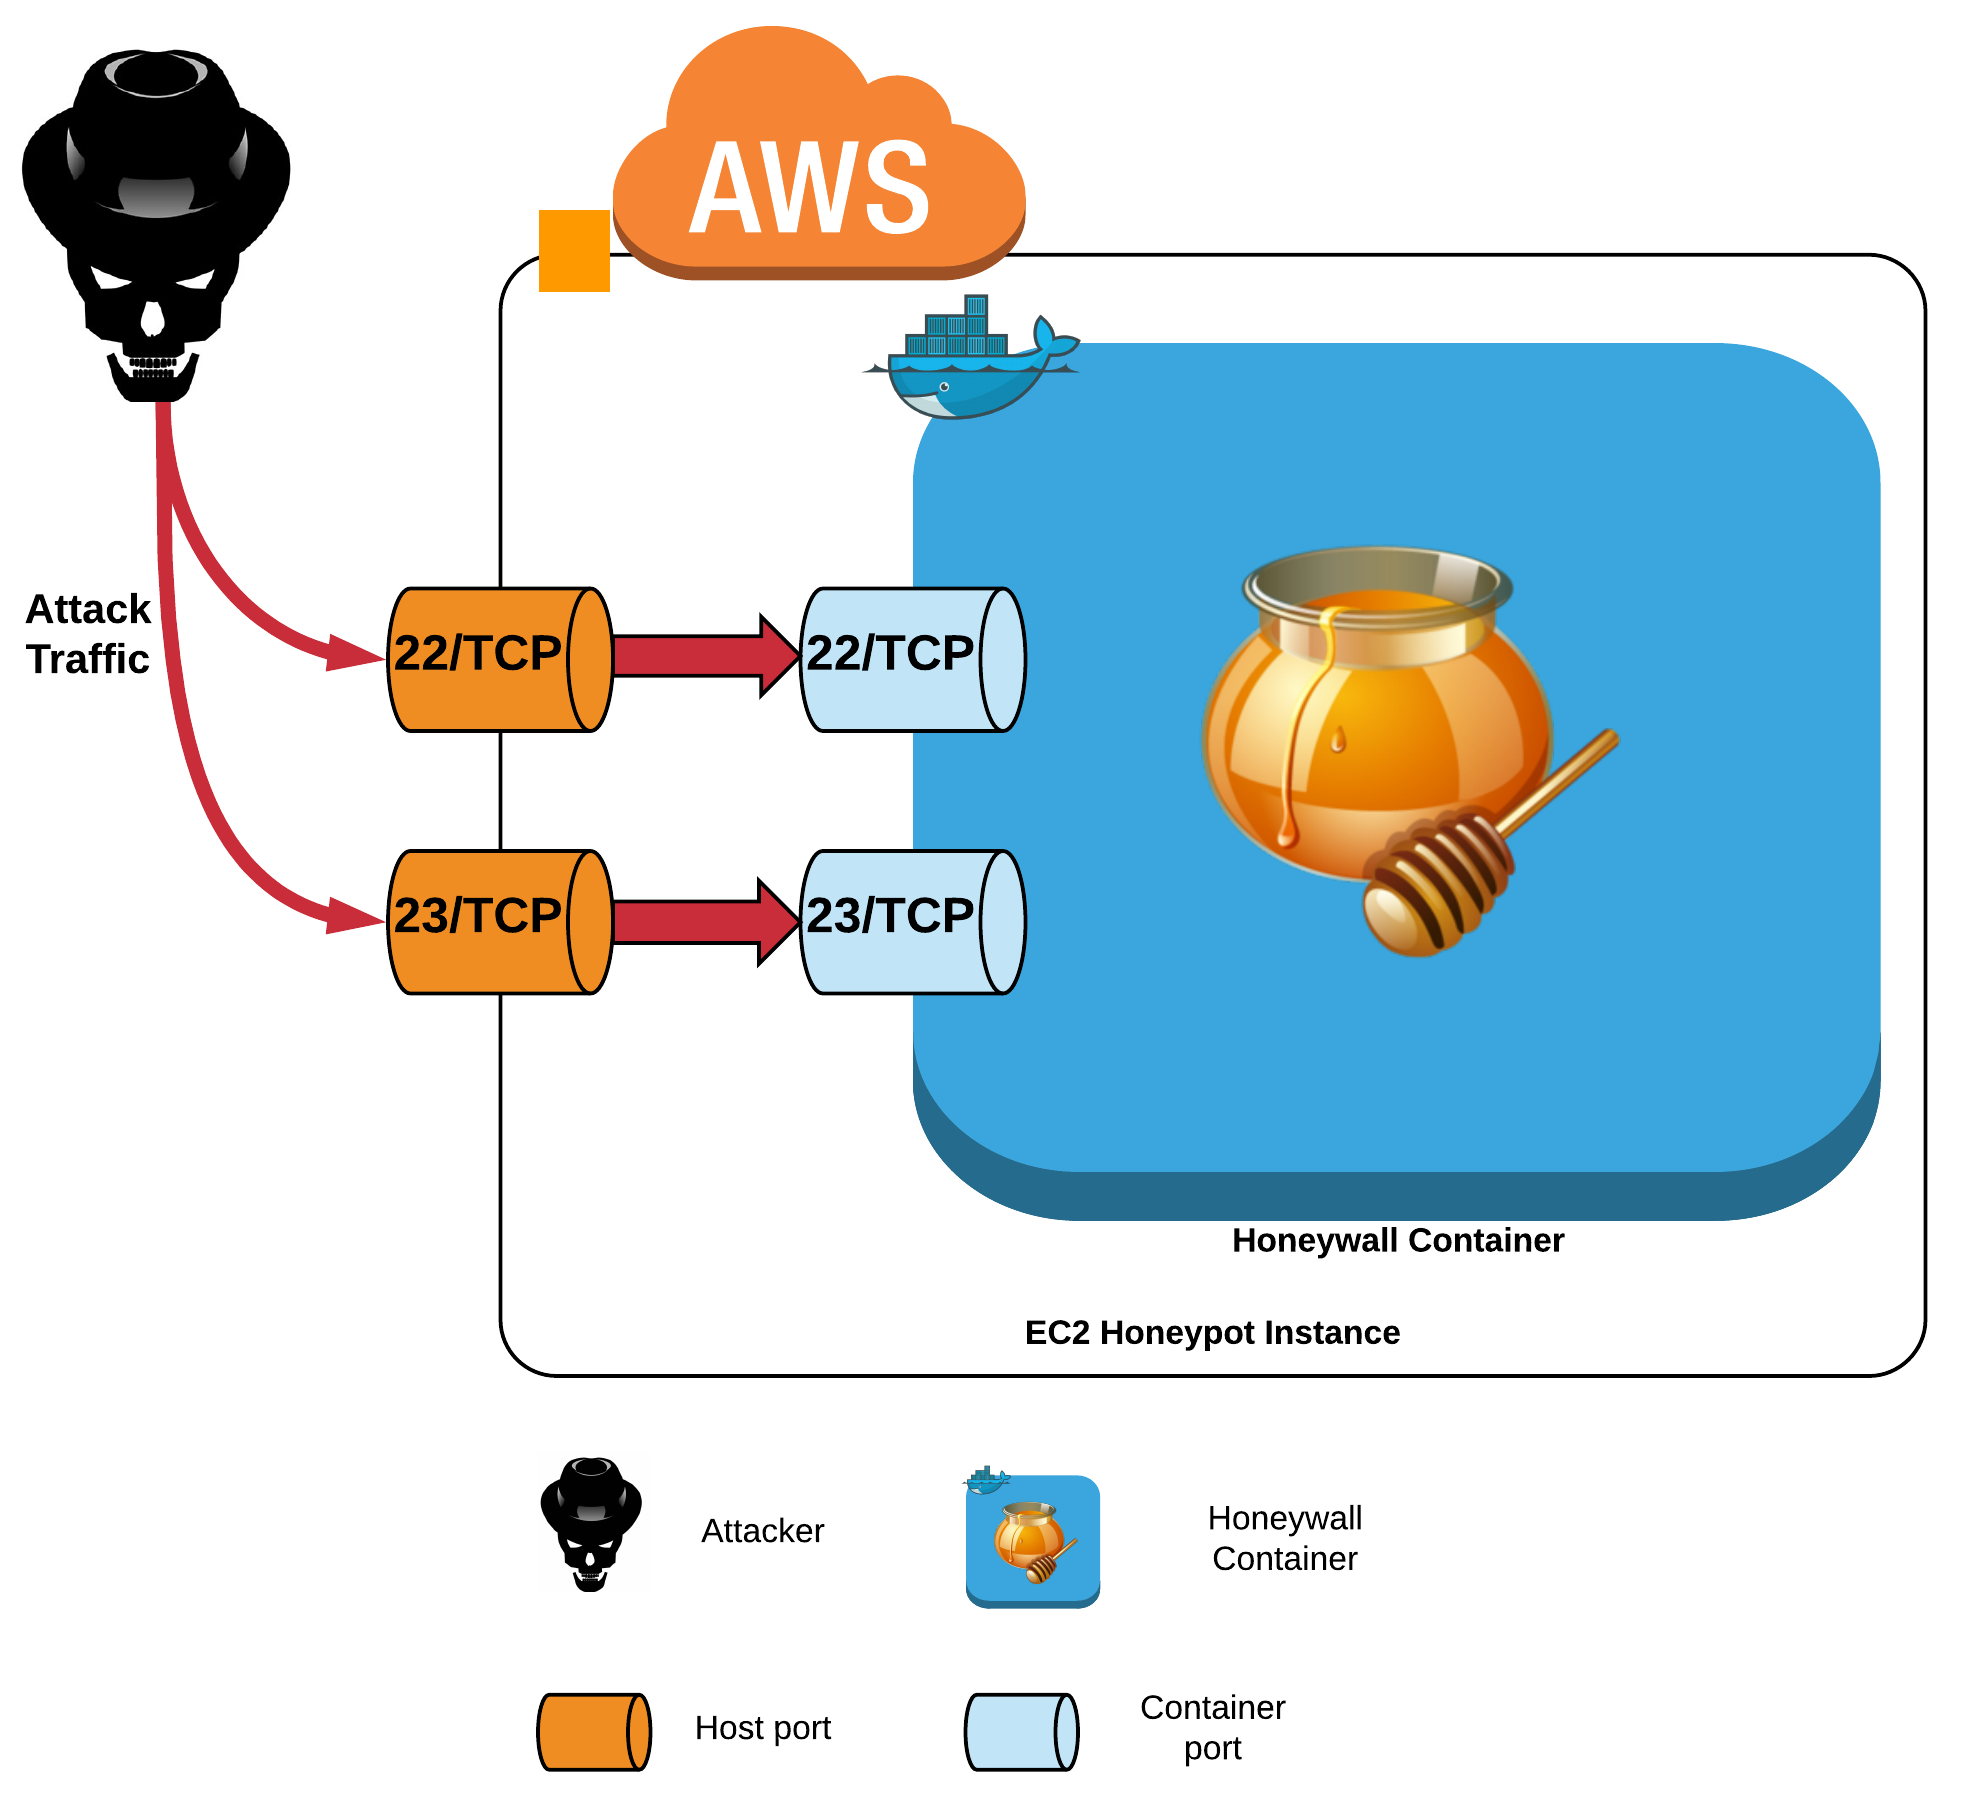
\includegraphics[width=125mm, scale=1]{Images/Port_mapping_for_the_honeywall_container.png}
      \caption{Port Publication on the Honeywall Container} 
      \medskip
      \small
		An illustration of the publication of ports 22/TCP, 23/TCP on the honeywall container to ports 22/TCP, 23/TCP on the host. Any traffic received by the host on these ports is mapped directly to the corresponding ports on the container, essentially making these container ports directly available from the Internet.
\label{fig:HoneywallPortPublication}
\end{figure}

%\includewidefigure{HoneywallPortPublication}{Port Publication on the Honeywall Container}{An illustration of the publication of ports 22/TCP, 23/TCP on the honeywall container to ports 22/TCP, 23/TCP on the host. Any traffic received by the host on these ports is mapped directly to the corresponding ports on the container, essentially making these container ports directly available from the Internet.}{Images/Port_mapping_for_the_honeywall_container.png}

A separate function was added to the \textit{do\_honeypot.sh} script to create and launch this container as distinct from an ordinary Cowrie container which would not be publishing these ports. 





%
% DOCKER HONEYNET
%
\subsection{The Docker Honeynet}
The Docker honeynet is one of the novel components of the system design, and would consist of new Docker network with a number of Cowrie containers connected to it. The honeywall Cowrie container would act as a gateway between the EC2 honeypot instance and this Docker network, meaning that it would need to have virtual interfaces on both the \textit{bridge} Docker bridge network and the new Docker network hosting the other Cowrie containers.

\subsubsection{Defining a Docker Bridge Network}
    The new Docker network that would host the Cowrie honeypot containers was defined as a bridge network with address 10.0.0.0/8\footnote{A /8 subnet can have up to 16,777,214 nodes with different IPv4 addresses. Though this scale is certainly not required here, the fact that these subnets are supported in Docker allows for many containers to belong to a single network.}. This network address was chosen because it is an address reserved for use in private networks, i.e. those not directly connected to the public internet. \cite{rfc1918}  The network was given the name \textit{dmz} corresponding to the notion of a DMZ explained in \textit{Section \ref{MotivationsForIntrusionDetection}}.
    
    In the \textit{do\_honeypot.sh} deployment script, a new function was added to allow a user to automatically define this network without needing to provide configuration details. This function can be seen in \textit{Snippet 5.2}.
    \mbox{}\\
    \includecode{Script to Create the Docker DMZ Network}{This script shows the commands used to create the virtual Docker bridge network, \textit{dmz}. The script uses the \textit{docker network ls} command to check whether the network already exists, and if not creates it. The \textit{-d bridge} argument specifies that the Docker bridge network driver should be used to create the network, and the \textit{attachable} argument indicates that containers can be added to the network manually on-the-fly.}{Code_snippets/create_dmz_net.sh}\label{create-dmz-net-code}

\subsubsection{Connecting Containers to the Honeynet}
% Specify IP addresses for everyone on the network
% What is the visibility of each container on the network? What ports are open (22, 23) and who can see that?
    
    As discussed in \textit{Section \ref{DockerSecurityConsiderations}}, ensuring that the honeypot containers did not have any unnecessary networking capabilities needed to be considered in the implementation. By specifying that Cowrie containers should be connected to the \textit{dmz} network as part of the \textit{do\_honeypot.sh} deployment script, they would not be added to any other networks by the Docker engine, ensuring this. 
    
    Connecting these containers to the \textit{dmz} network involved adding a single extra argument to the \textit{docker create} CLI commands for the Cowrie and honeywall containers in the \textit{do\_honeypot.sh} script: \textit{--network ''dmz''}. When executed, the \textit{docker create} command would now randomly assign an IP address on the \textit{dmz} network to the Cowrie containers, and a specific IP address to the honeywall container\footnote{The address 10.0.0.254/8 was specified for the honeywall container, since this address is commonly configured as the address for routing devices in real-world networks and so was determined to add to the attractiveness of this container from an attackers perspective.}. 
   

\subsubsection{Network Configuration of the Honeywall Container}
The function of the honeywall Cowrie container differs from that of other Cowrie containers in that it should act as a gateway between the Cowrie honeynet and the EC2 host. This requires that the honeywall Cowrie container have two virtual network interfaces: One on the default \textit{bridge} network in order to communicate with the host instance, and the other on the \textit{dmz} honeynet.

Configuring the honeywall container as the gateway for the \textit{dmz} network was not as easy to achieve as it first seemed. The issue encountered was as follows:
    \begin{itemize}
    \item The IP address of the network gateway must be specified at the time of creation of the network. It is not possible to specify a network component as the gateway, i.e. the honeywall container cannot be specified as the gateway, but in theory its IP address could be.
\item Clearly, a container cannot have an IP address for a network that has not already been created: Thus, a container cannot first be given an IP address and then that IP address specified as the gateway during the creation of the network.
    \end{itemize}
    
    In essence, it is not possible through Docker to the honeywall container as the gateway for the \textit{dmz} network, since the network must already be defined with a gateway before the container can be a part of it in the first place. As an issue for which no reference documentation existed, overcoming this issue took substantial troubleshooting and trial-and-error. Eventually, it was resolved by manual manipulation of the \textit{iptables} rules and routing table configuration once the container was running.
    
    To ensure that this configuration would always be present when this container is launched in future,  a new Dockerfile was created for the honeywall container. The Dockerfile contained the same configuration options as that of the other Cowrie containers, but used a different entrypoint script at runtime that would configure the \textit{iptables} rules and routing tables.


\subsection{Design Pivot: A New High-Interaction Honeypot}\label{DesignPivot1}
     
    It was discovered during the configuration of the honeywall container that the Cowrie honeypot does not have outbound networking capabilities such that it can make outbound SSH or telnet connections. This was something that was not fully understood about the Cowrie honeypot initially\footnote{It was understood before beginning the implementation of the system that the Cowrie honeypot \textit{did} have this functionality, since it is known that issuing a \textit{wget} download request inside the Cowrie honeypot downloads the requested resource and computes its SHA-checksum whilst appearing to the attacker to have failed. Such functionality would require the honeypot to make an outbound network connection, and the same approach was assumed to have been taken to the implementation of the SSH and telnet services in Cowrie.}, unearthed through implementation issues and verified by the maintainer of the Cowrie honeypot, Michel Oosterhof. In response to an email query on the subject, he outlined the following:
    
\begin{center}
''\textit{Cowrie by design doesn't do any outbound connections from within the honeypot... So if you want communicatoin between the instances, that'll be a fairly significant programming exercise. You'll need to learn some Python/Twisted and basically implement an SSH/Telnet client inside Cowrie that can connect to the next instance. Or you'll have to create some way to bypass this and make it appear that this is what happens to the attackers.}''
\end{center}    

When this realisation was made, the original approach to implementing the honeynet required immediate re-evaluation. The ability to make outbound network connections from the honeywall container is essential so that an attacker can access the honeynet. However, the honeywall container should also be a maximally restricted environment to minimise the risk of attack propagation outside of the system. These considerations motivated a re-assessment of the system design.

\subsubsection{Re-Evaluation of Initial Design \label{DesignReEvaluation}}
Given the time within which the research was being conducted, it would not be possible to extend the Cowrie source code to give the honeypots the ability to make outbound network connections over SSH and telnet. Instead, a decision was made to implement a new high-interaction Docker honeypot\footnote{It was decided to implement an entirely new high-interaction honeypot since there are very few high-interaction honeypots that exist, and none that were found to be actively maintained. In their survey of honeypot software, Nawrocki \textit{et al.} found that the majority of honeypot solutions are low-interaction, and that when it comes to high-interaction solutions ''only few exist''. \cite{Nawrocki2016}} to facilitate the propagation of attacks beyond the honeywall: A component referred to hereafter as the \textit{router container}. 

As a high-interaction honeypot, the router container faced an array of new challenges.

\begin{itemize}
\item Since attackers would no longer be interacting with an emulated environment inside the Docker container, real libraries and toolkits would have to be made available to encourage them to interact with the system.
\item The Cowrie application gives a simple configuration option for specifying username-password combinations that should be allowed or disallowed for authentication by the honeypot. This is not so easy to replicate in a real system, where a user account can only be configured to accept either (i) a single correct password\footnote{This also presents an additional issue, since if only a single correct password is permitted per user the probability of an attacker actually attempting this password is low.} or (ii) no password to authenticate a login. 
\item Attackers will always seek to gain root access to a system in order to have unrestricted control over it. Cowrie emulates this root access effectively, but this cannot be falsified in a real system and would require giving real root privileges to the attacker\footnote{This would be required since if attackers are not permitted to login as root, it is less probable that any attackers will ever reach the Cowrie honeynet.}. This is highly risky, since there is no limitation on what actions they can then perform inside the system.
\item An approach to logging network traffic and command execution would need to be identified in order to capture attack data, since these capabilities of the Cowrie honeypot would also no longer be available to this container.
\end{itemize} 

The approaches taken to deal with each of these new difficulties are detailed in the subsequent sections.

\subsubsection{Defining a New Container Image}
Since the requirements of the router container would be significantly different to that of the highly-restricted Cowrie container, a new Docker image definition was required. 

It was decided that in order to have access to a wide variety of powerful Linux utilities\footnote{This variety would be required to facilitate an attacker in accessing whatever utilities they required in order to progress with their attack: It would be undesirable for the attacker to disconnect from this container without progressing to the Cowrie honeynet, since experimental data would then never be captured by the honeynet.}, the \textit{ubuntu:latest} Docker base OS image would be used as a foundation for the router container image. The container would also need to expose ports 22/TCP and 23/TCP as with the Cowrie containers, and so these were specified in the Dockerfile using the \textit{EXPOSE} command.

The most generic Linux utilities that were specified as part of the Docker-Cowrie image were also included in this new image: In particular, the \textit{apt-utils} and \textit{build-essential} packages, which are required as basic utilities in almost all Debian-based Linux environments.

Once the basic Dockerfile was defined, the \textit{do\_honeypot.sh} script was updated to use the new router container image instead of the old honeywall container image. The \textit{docker create} arguments for adding the container to the \textit{dmz} network and publishing ports 22/TCP and 23/TCP to the host interface were left unchanged, since the router container would still require this configuration.

\subsubsection{Configuring SSH and Telnet}
Since there was now no emulation of SSH and telnet connectivity, it was necessary to install and configure utilities for these on the router container. The installation of the required packages was specified as part of the router container Dockerfile, and their runtime configuration properties specified in an entrypoint script.

\paragraph{SSH}\mbox{}\\
The installation of the \textit{openssh-server} utility was specified in the Dockerfile. Then, the entrypoint script was used to update the configuration of the SSH daemon \textit{sshd} to facilitate SSH logins to the container. Some noteworthy configurations specific to enabling easy access by attackers to the container include the following:

\begin{itemize}
    \item The \textit{PermitRootLogin} field was updated to allow SSH logins as user \textit{root};
    \item The \textit{PasswordAuthentication} field was updated to allow authentication by password and not just by using an encryption key;
    \item The \textit{PermitEmptyPasswords} field was updated to allow authentication with an empty password, if this was valid for a particular user.
\end{itemize}

Lastly, the entrypoint script was updated to restart so that the updated configuration would take effect.

\paragraph{Telnet}\mbox{}\\
The installation of the \textit{telnet}, \textit{openbsd-inetd } and \textit{telnetd} package utilities were also added to the Dockerfile. A number of configuration steps were also added in the entrypoint script to be applied at container runtime: In particular, the allocation of a number of \textit{ttys}\footnote{In Linux systems, a tty is a representation of a text input/output device to the system, such as a terminal session.} to allow multiple simultaneous telnet sessions to take place. 

A telnet configuration file called \textit{telnet} was also added to the container, which included a number of essential configuration options as well as some logging parameters. This required use of the Dockerfile \textit{COPY} command to copy the file into the container's \textit{/etc/xinetd.d} directory. As with the configuration of SSH, the telnet daemon is restarted to allow the changes to take effect.

\subsubsection{Device Banner Configuration}
As part of the \textit{enumeration} phase of an attack, an attacker will often use a scanning tool such as \textit{Nmap} or \textit{Masscan} to fingerprint the target system. These scanning tools usually send a message probe over particular protocols with the intention of receiving an acknowledgement (ACK) from the target, allowing the attacker to deduce some properties of the system. In the case of IoT devices, being able to fingerprint the device type and model is very useful to an attacker in identifying a vulnerable target, and so the router container needed to be capable of presenting such information.

There are two primary messages that are presented to those initiating a user authentication connection with a Linux-based system: The \textit{issue.net} and \textit{mot.d} files.
\begin{itemize}
\item \textbf{issue.net / issue}

        This file is used to set the banner that is sent in a protocol negotiation, e.g. for a client requesting to connect to the system via telnet, this would be the information that is used to greet the client prior to the login step. For SSH, this file is called \textit{issue} whereas for telnet the file is called \textit{issue.net}.

\item \textbf{motd / legal}

        This file is used to display a message to a client after they have successfully logged into the system. Often, administrators will use this to present a notice about permitted uses of the system after a user has successfully logged in. For SSH, this file is called \textit{legal} whereas for telnet the file is called \textit{motd}.
		\end{itemize}
        
In the Dockerfile for the router container, commands were added to copy customised \textit{issue.net}, \textit{issue}, \textit{legal} and \textit{motd} files defined on the host into the container. Some additional updates were then made to the entrypoint script so that these banners would be presented in connection negotiations. Figure {fig:router-telnet-banner} shows how these banners appear to an individual attempting to gain access to the system via telnet.

 \begin{figure}[ht]
      \centering
      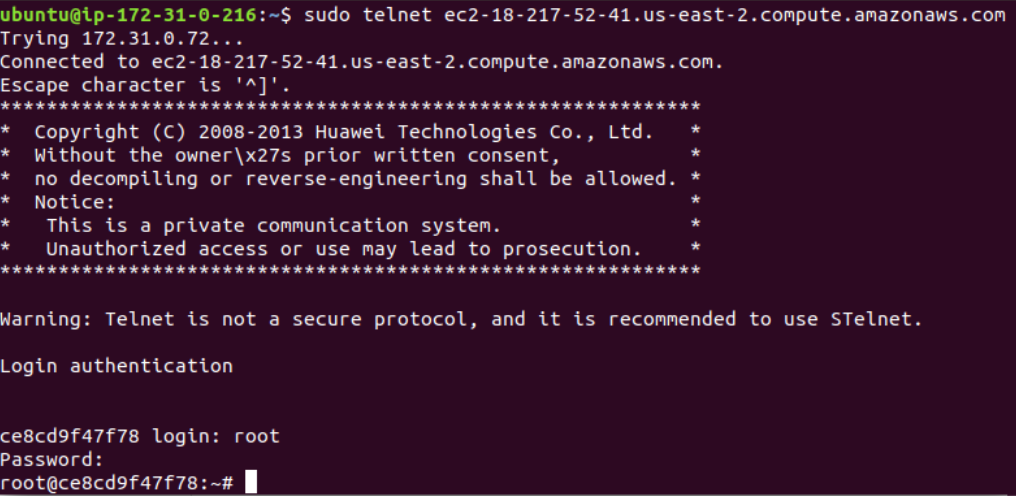
\includegraphics[width=160mm, scale=1]{Images/logging_into_router_container_with_telnet.PNG}
      \caption{The Router Container Honeypot Telnet Banner} 
      \medskip
      \small
		This screenshot shows a login attempt via Telnet to the EC2 honeypot server instance. It can be seen that a banner advertising a Huawei device is presented as part of the login prompt. It can be observed that the ''attacker'' proceeds to successfully log in as user \textit{root}.
\label{fig:router-telnet-banner}
\end{figure}

%\includewidefigure{router-telnet-banner}{The Router Container Honeypot Telnet Banner}{This screenshot shows a login attempt via Telnet to the EC2 honeypot server instance. It can be seen that a banner advertising a Huawei device is presented as part of the login prompt. It can be observed that the ''attacker'' proceeds to successfully log in as user \textit{root}.}{Images/logging_into_router_container_with_telnet.PNG}

\subsubsection{Privileges and Authentication}
As identified in \textit{Section \ref{DesignReEvaluation}}, for an attacker to interact with the system they would need to believe that they have gained root-level access to the router container. This is not something that can be falsified without the use of an emulated environment like Cowrie, and so the decision was made to allow root access by default for all user accounts on this container. 

A related issue is the fact that arbitrary user-name password combinations could not be accepted in the same way on a real Linux environment as they could be with the emulated Cowrie environment. 
\begin{itemize}
\item In  order for an attacker to log in to the router container under a particular user, an account needs to exist for that user.
\item  As well as this, it is only possible to specify one valid password per user account.
\end{itemize} 
The reality of this was that the number of username-password combinations that could be accepted for this honeypot would be greatly restricted. 

The solution to these issues was to define a number of user accounts with usernames commonly observed in brute-force authentication attacks, and give each of these users root privileges by default. Since the exact username-password combinations used in the system would be determined through experiments, a single account for user \textit{admin} was created as part of the Dockerfile. 

In order to give root privileges to user accounts, they needed to be declared as \textit{sudo} users\footnote{A sudo user is one which has root privileges on the system, with unrestricted read, write and execute capabilities.}. This involved the installation of the \textit{sudo} package as part of the Dockerfile, and the use of the \textit{COPY} command in the Dockerfile to copy a pre-configured sudoers file into the container from the host. This sudoers file was configured such that it granted root-level privileges to the \textit{admin} user for all utilities in the container.


This configuration should now allow an attacker authenticated as user \textit{admin} to successfully carry out unrestricted activities inside the container.


\subsubsection{Logging Attack Events}
As with the Cowrie honeypot containers, it was essential that the router container could monitor the activities of an attacker on the system. This container is a high-interaction honeypot: A fully-fledged container with a real networking stack, toolkits and file system. As described in \textit{Section \ref{HoneypotInteractivityLevels}}, these honeypots offer the highest value in terms of capturing information about interactions with attackers since attacker activities are usually unrestricted. The most important elements of attack activities that needed to be captured in logging were the commands executed by attackers, and details of the attacker's connection session. 

 \paragraph{Network Event Logging}\mbox{}\\
  The most commonly used logging utility for network events is \textit{syslog}. Syslog is IETF standard Linux logging utility, which logs network and process events that occur on a system. It is heavily used by system administrators for system management and security auditing purposes. \cite{rfc5424} It was identified as a straight-forward logging solution for capturing information about attacker connections to the router container, since it is capable of capturing logging information for both SSH and telnet.
  
 In order to use syslog, the \textit{rsyslog} package was added to the Dockerfile as part of the image installation for the router container. A custom-defined configuration file called \textit{rsyslog.conf} was then added to the container image, and in the entrypoint script for the container the \textit{rsyslog} utility was launched\footnote{The launching of the \textit{rsyslog} utility was the last operation specified in the entrypoint script in order. This was to ensure that none of the environment configuration updates applied by the script were included in the log files, meaning that if an attacker was to inspect the syslogs on the container they would not see any records relating to the configuration of the environment, reducing the likelihood of them fingerprinting it as a honeypot.}. 
  
 In order to persist the logs generated by \textit{rsyslog} inside the router container, a volume was mounted to the router container in the \textit{/var/log} directory as part of the function to create the router container in the  \textit{do\_honeypot.sh} script. SSH and telnet events are logged to a number of different log files within this directory, including \textit{auth.log}, \textit{messages}, \textit{secure} and \textit{syslog}.
    

	  \paragraph{Keylogging}\mbox{}\\
      \textit{Logkeys} is an open-source Linux keylogger. \cite{LogkeysGithub} As one of the only identified Linux keyloggers freely available and relatively recently maintained, it was originally selected as a keylogging solution for monitoring the activities of attackers inside the router container.
      
      There were a number of significant difficulties encountered with the use of \textit{logkeys}: Seemingly, these were due to its incompatibility with Docker.
      % event interface of the Linux input subsystem
      \begin{itemize}
      \item There was no single reference which specified all of the dependencies required to be installed in order for \textit{logkeys} to operate. Since Docker containers take a lean approach to sharing libraries and packages with their host\footnote{In general, Docker base images such as the Ubuntu Docker image are shipped only with the bare minimum of packages included, and require a lot of additional packages to be installed in order to run and manage applications.}, many of these dependencies had to be installed from the \textit{apt} repositories. These dependencies were eventually identified through investigating \textit{dumpkeys}, an ancient Linux keylogger which shares a lot of the same library dependencies. \cite{dumpkeysKeyloggerManpage}
      \item The fact that \textit{logkeys} depends on being able to reference a keyboard device driver on the host machine presented a number of issues to the use of keylogging. Input device drivers are stored in Linux systems in a device file, which appears as an ordinary file under the \textit{/dev/input} directory. Although a \textit{--device} argument exists for the \textit{docker create} CLI command which can be used to reference a device driver on the host, the keyboard input device remained inaccessible by \textit{logkeys} inside the Docker container despite over a week of dedicated effort.
      \end{itemize}
 
 After exhausting all identified venues for implementing keylogging with \textit{logkeys}, a number of additional options were investigated.
 
 \begin{itemize}
 \item The idea of using the Linux \textit{.bash\_history} file for keylogging was explored. This file is created by the Bash utility, and captures all executed command-line inputs. This initially seemed a reasonable approach to keylogging: However, the fact that commands are not logged with timestamps would render the data largely unusable for identifying distinct attack sessions, making this an unsuitable approach.
 \item A manual keylogging approach was attempted, inspired by a recommendation on the online forum \textit{askubuntu.com}. \cite{ManualKeyloggingAskUbuntu} This keylogging approach involved using pure shell command manipulation, leveraging off SSH and telnet environment variables generated as part of \textit{syslog} network event logging. However, this approach was found to be unreliable and brittle, and so was also abandoned.
\end{itemize}
 
With the time constraints involved in the implementation of the system, the idea of keylogging was eventually put to one side as future work to improve the router container honeypot. 
     
\subsubsection{Package Utilities}
As identified in the design re-evaluation in \textit{Section \ref{DesignReEvaluation}}, a number of Linux utilities that an attacker would expect to find in a legitimate system needed to be made available  in the container, since the emulation of these utilities provided by Cowrie were no longer available. In particular, it was important to facilitate an attacker in probing the \textit{dmz} network in order to discover the Cowrie honeypot containers, and so providing common networking packages was a must.

The initial utilities that were added to the Dockerfile for the router container were \textit{net-tools}, \textit{nmap}, \textit{traceroute}, \textit{inetutils-ping}, \textit{iptables }and \textit{tcpdump}. These are all networking packages that would allow an attacker to perform actions such as viewing and manipulating the container's routing table, scanning nearby hosts and capturing packets on the network. 
   
\subsection{Finalising the Docker Honeynet}
Now that all required components of the Docker honeynet had been implemented, all that remained was to ensure that the network configuration was operating correctly. An attacker should be able access the router container from the public internet and from there, interact with any available Cowrie containers on the \textit{dmz} network. 

The targeted network configuration for the deployment is illustrated in figure \ref{fig:honeypot-instance-networking}.

\begin{figure}[ht]
      \centering
      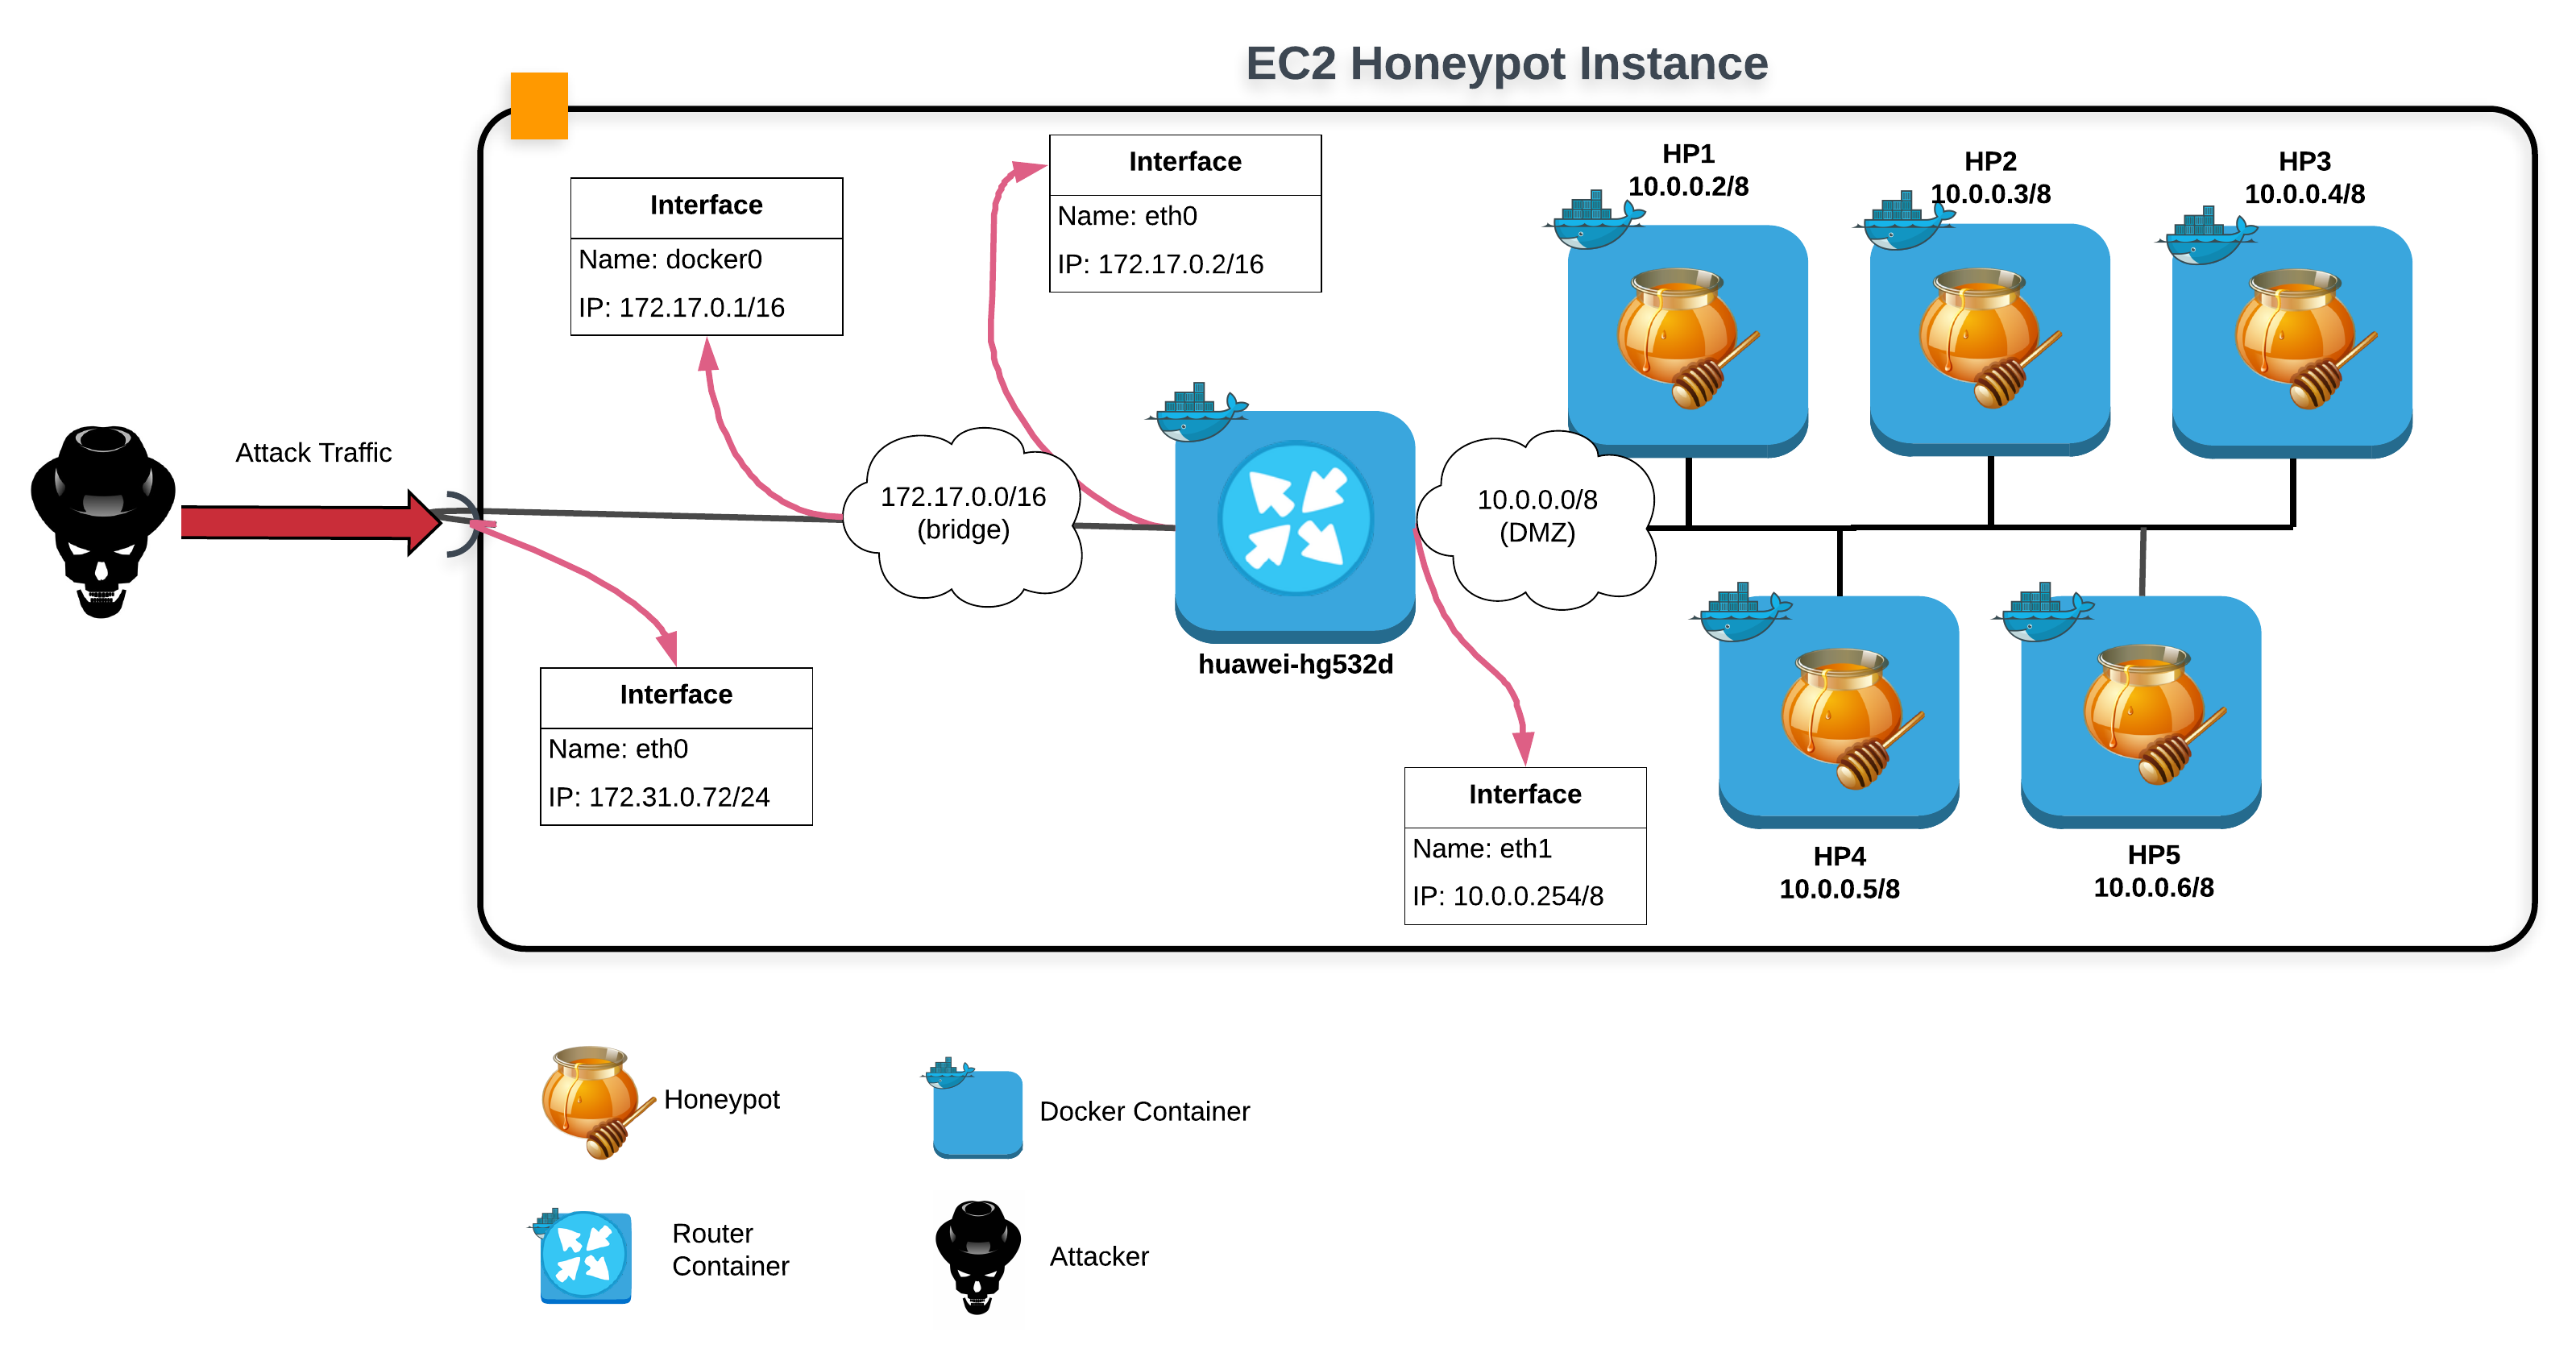
\includegraphics[width=160mm, scale=1]{Images/Honeypot_Instance_Networking.png}
      \caption{Docker Network Configuration of the EC2 Honeypot Instance} 
      \medskip
      \small
		This figure illustrates the desired network configuration for the honeynet deployment on the EC2 honeypot instance. It can be observed that there are two bridge networks: \textit{bridge} and \textit{dmz}. The host instance is forwarding its incoming traffic on ports 22/TCP and 23/TCP to the \textit{docker0} virtual interface on the \textit{bridge}. This interface connects the host to the router container's virtual interface \textit{eth0}. The router container also has a second virtual interface, \textit{eth1} which connects it to the \textit{dmz} network. It is through this interface that the Cowrie honeypots in the \textit{dmz} network can be accessed.
\label{fig:honeypot-instance-networking}
\end{figure}

%\includewidefigure{honeypot-instance-networking}{Docker Network Configuration of the EC2 Honeypot Instance}{This figure illustrates the desired network configuration for the honeynet deployment on the EC2 honeypot instance. It can be observed that there are two bridge networks: \textit{bridge} and \textit{dmz}. The host instance is forwarding its incoming traffic on ports 22/TCP and 23/TCP to the \textit{docker0} virtual interface on the \textit{bridge}. This interface connects the host to the router container's virtual interface \textit{eth0}. The router container also has a second virtual interface, \textit{eth1} which connects it to the \textit{dmz} network. It is through this interface that the Cowrie honeypots in the \textit{dmz} network can be accessed.}{Images/Honeypot_Instance_Networking.png}


\subsubsection{The Docker \textit{bridge} Network Configuration}
For the router container to be accessible from the public internet, its configuration on the \textit{bridge} Docker network needed to  be set up to facilitate this. The first step was to inspect the configuration of the \textit{bridge} network and the routing table on the EC2 instance itself. The desired configuration is illustrated in figure \ref{fig:router-container-config}.

\begin{figure}[ht]
      \centering
      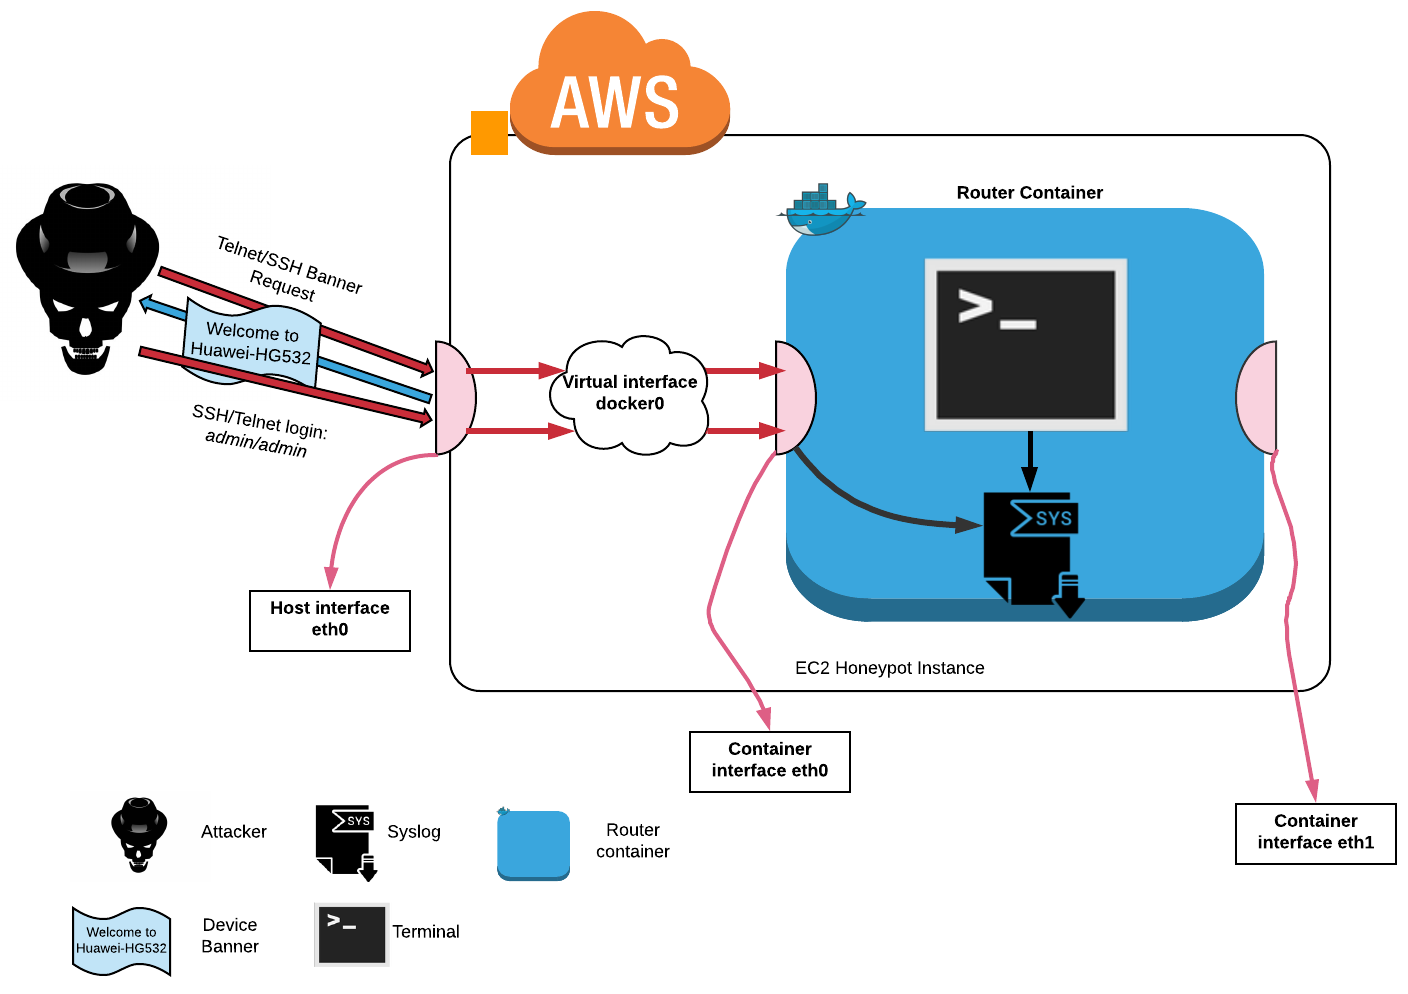
\includegraphics[width=160mm, scale=1]{Images/Router_container_config.png}
      \caption{Routing of Attack Traffic to the Router Container} 
      \medskip
      \small
		An illustration of the desired routing of attack traffic from the host network interface to the router container. The attacker is shown to attempt a brute-force authentication attack over either SSH or telnet, which is forwarded from the real host interface \textit{eth0} to the \textit{docker0} virtual interface on the \textit{bridge} network. From this interface, the traffic is forwarded to the \textit{eth0} router container interface. For the response to the attacker, the flow of traffic through the network is in reverse order through these interfaces. 
\label{fig:router-container-config}
\end{figure}

%\includewidefigure{router-container-config}{Routing of Attack Traffic to the Router Container}{An illustration of the desired routing of attack traffic from the host network interface to the router container. The attacker is shown to attempt a brute-force authentication attack over either SSH or telnet, which is forwarded from the real host interface \textit{eth0} to the \textit{docker0} virtual interface on the \textit{bridge} network. From this interface, the traffic is forwarded to the \textit{eth0} router container interface. For the response to the attacker, the flow of traffic through the network is in reverse order through these interfaces. }{Images/Router_container_config.png}

The internal routing table of the EC2 honeypot instance can be seen in table \ref{table:host-routing-table}, showing the networks associated with its physical network interface \textit{eth0} and Docker virtual network interface \textit{docker0}. By design, the host cannot interface directly with the \textit{dmz} bridge network: As discussed in \textit{Section \ref{DockerSecurityConsiderations}}, by preventing the host and containers from being connected to unnecessary networks the risk of these systems being compromised in an attack is minimised.

\begin{table}[!h]
	\begin{center}
		\begin{tabular}{|c|c|c|c|c|c|c|c|} 
			\hline
			\bf Destination  & \bf Gateway  & \bf Genmask  & \bf Flags & \bf Metric & \bf Ref & \bf Use & \bf Iface \\
			\hline
			0.0.0.0 & 172.31.0.1 & 0.0.0.0 & UG & 0 & 0 & 0 & eth0  \\
            172.17.0.0 & 0.0.0.0 & 255.255.0.0 & U & 0 & 0 & 0 & docker0  \\
            172.31.0.0 & 0.0.0.0 & 255.255.240.0& U & 0 & 0 & 0 & eth0  \\
			\hline
		\end{tabular}
	\end{center}
	\caption[Routing Table of the EC2 Honeypot Instance]{The routing table produced by the command \textit{route -n} executed on the honeypot instance, which hosts the Docker honeynet. Two interfaces can be observed: \textit{eth0} and \textit{docker0}. \textit{eth0} connects the host to the 172.31.0.0/24 network, which is an external network managed by AWS. The \textit{docker0} interface corresponds to a default bridge network called \textit{bridge} with address 172.0.0.0/16, which containers are connected to by default if not specified otherwise.}	
	\label{table:host-routing-table}
\end{table}

By executing the command \textit{docker network inspect bridge}, the properties of the Docker \textit{bridge} network can be inspected. The output of executing this command can be seen in figure \ref{fig:docker-network-inspect-bridge}. It can be seen that there is only 1 container on this network, corresponding to the router container \textit{router}. If the command \textit{docker container inspect router} is subsequently executed, the output obtained\footnote{The volume of output generated by this command is not feasible to include as a figure in this document, and so a description of the most important contents of the output was deemed sufficient.} demonstrates the following expected properties:

\begin{itemize}
\item The \textit{router} container is connected to the \textit{bridge} network with an IP address of 172.17.0.2/16;
\item The router container is also connected to the\textit{dmz} network with an IP address of 10.0.0.254/8;
\item Ports 22/TCP and 23/TCP of the \textit{router} container are published to ports 22/TCP and 23/TCP of the host interface.
\end{itemize}

\begin{figure}[ht]
      \centering
      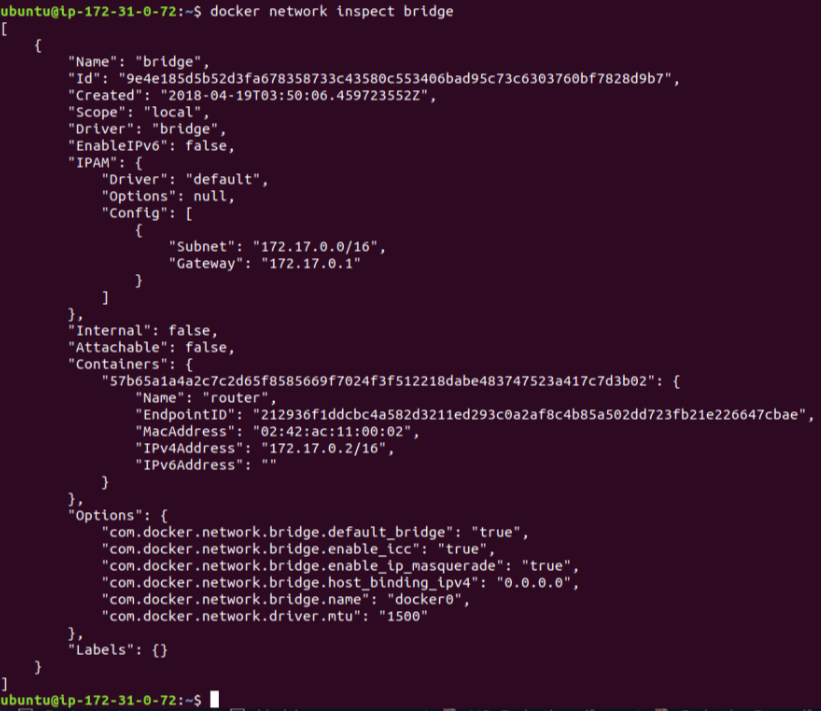
\includegraphics[width=160mm, scale=1]{Images/docker_network_inspect_bridge.PNG}
      \caption{Console Output of \textit{docker network inspect bridge}} 
      \medskip
      \small
		An image showing the console output obtained by executing the command \textit{docker network inspect bridge}. It can be observed that there is only 1 container on this network: The \textit{router} container. 
\label{fig:docker-network-inspect-bridge}
\end{figure}

The correct routing of attack traffic through the \textit{bridge} network could be tested from outside the EC2 honeypot server instance, by connecting over SSH or telnet to the instance and verifying that the router container login prompt is presented. Figure \ref{fig:ssh-to-router-successful} shows the console output when an SSH connection is made to the EC2 honeypot server instance, demonstrating the correct routing of this traffic to the router container.

\begin{figure}[ht]
      \centering
      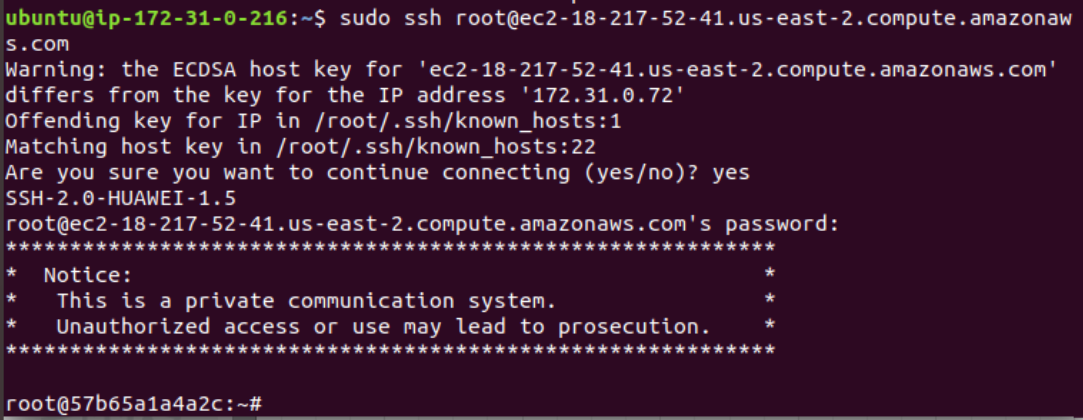
\includegraphics[width=160mm, scale=1]{Images/ssh_to_router_successful.PNG}
      \caption{Attempted SSH Login to the Router Container} 
      \medskip
      \small
		An image showing the console output obtained when a connection attempt is made over SSH to the EC2 honeypot instance. It can be observed that a Huawei banner is presented, and that the attacker is permitted to log in as \textit{root}. 
\label{fig:ssh-to-router-successful}
\end{figure}





\subsubsection{The Docker \textit{dmz} Network Configuration}
To verify that attack traffic could reach the Cowrie containers in the \textit{dmz} network,  the configuration of the router container and the \textit{dmz} network needed to be verified. An attacker, once inside the router container, should be able to connect through an interface on the router container to any Cowrie container on the \textit{dmz} network. The desired configuration is illustrated  in figure \ref{fig:cowrie-honeynet-container-config}.

\begin{figure}[ht]
      \centering
      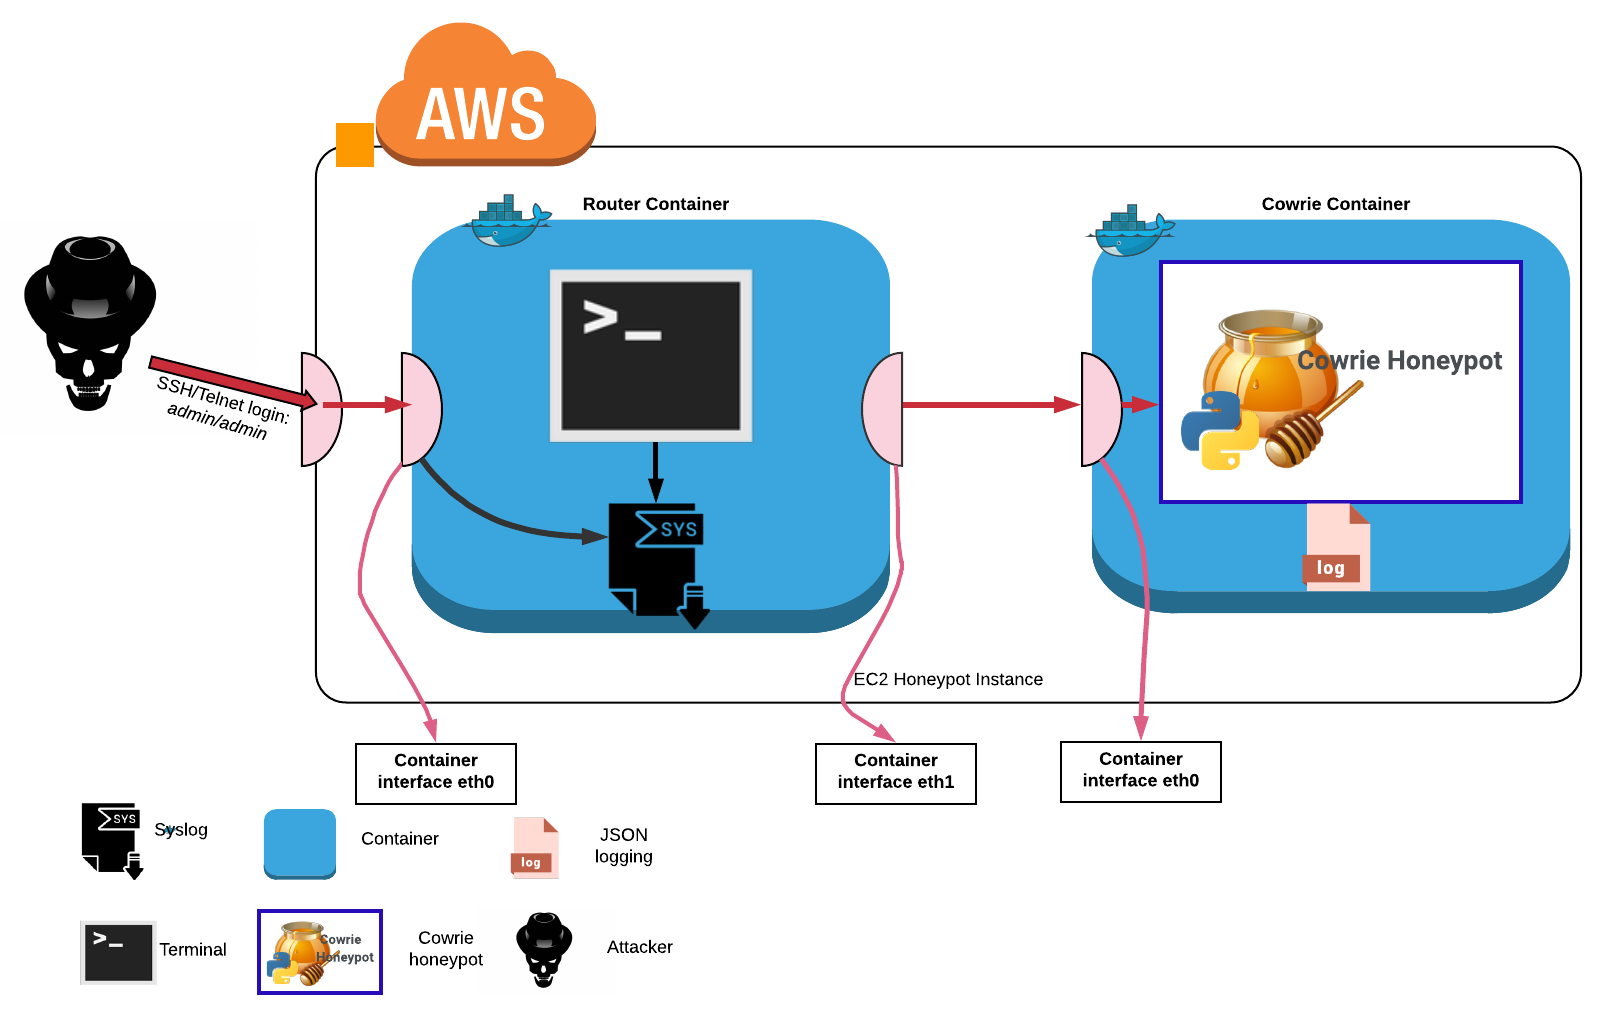
\includegraphics[width=160mm, scale=1]{Images/Cowrie_container_config.png}
      \caption{Routing of Attack Traffic to a Cowrie Container} 
      \medskip
      \small
		An illustration of the desired routing of attack traffic from the host network interface to a Cowrie container. Assuming that the attacker has already successfully compromised the router container through the process in figure \ref{fig:router-container-config},  they should be able to connect to the Cowrie container over SSH or telnet in the same way through the router container's \textit{eth1} interface on the \textit{dmz} network. 
\label{fig:cowrie-honeynet-container-config}
\end{figure}

%\includewidefigure{cowrie-honeynet-container-config}{Routing of Attack Traffic to a Cowrie Container}{An illustration of the desired routing of attack traffic from the host network interface to a Cowrie container. Assuming that the attacker has already successfully compromised the router container through the process in figure \ref{fig:router-container-config},  they should be able to connect to the Cowrie container over SSH or telnet in the same way through the router container's \textit{eth1} interface on the \textit{dmz} network. }{Images/Cowrie_container_config.png}[HD]

The internal routing table of the router container can be seen in table \ref{table:router-routing-table}, showing the networks associated with the container's two virtual interfaces \textit{eth0} and \textit{eth1}. These networks correspond to the \textit{bridge} network 172.17.0.0/16 and the \textit{dmz} network 10.0.0.0/8.

\begin{table}[!h]
	\begin{center}
		\begin{tabular}{|c|c|c|c|c|c|c|c|} 
			\hline
			\bf Destination  & \bf Gateway  & \bf Genmask  & \bf Flags & \bf Metric & \bf Ref & \bf Use & \bf Iface \\
			\hline
			0.0.0.0 & 172.17.0.1 & 0.0.0.0 & UG & 0 & 0 & 0 & eth0  \\
            10.0.0.0 & 10.0.0.254 & 255.0.0.0 & U & 0 & 0 & 0 & eth1  \\
            172.17.0.0 & 0.0.0.0 & 255.255.0.0 & U & 0 & 0 & 0 & eth0  \\
			\hline
		\end{tabular}
	\end{center}
	\caption[Routing Table of the Router Container]{The routing table produced by the command \textit{route -n} executed inside the router container. Two interfaces can be observed: \textit{eth0} and \textit{eth1}. \textit{eth0} connects the router container to the 172.17.0.0/16 \textit{bridge} network, whereas \textit{eth1} connects it to the 10.0.0.0/8 \textit{dmz} network.}	
	\label{table:router-routing-table}
\end{table}

From inside the router container, an attacker should be able to access a domain on the public internet in order to perform downloads to progress their attacks on the system. This is achieved through the configuration of Network Address Translation (NAT) rules in \textit{iptables}. The rules shown in snippet 5.3 were used to achieve this objective, enabling an attacker to perform downloads from external domains. This temporarily caused a diffiult-to-diagnose issue with the \textit{iptables} of the EC2 instance\footnote{The issue manifested as an inability to connect to containers on ports 22/TCP and 23/TCP, where Nmap would show these ports as being 'filtered'.}, which was eventually resolved by executing the command \textit{iptables -t nat --flush} to remove some conflicting NAT rules on the host.

\includecode{NAT iptables Rules}{The \textit{iptables} rules that were configured to enable NAT inside the router container.}{Code_snippets/NAT_iptables_rules.sh}\label{lst:nat-rules}

The routing table generated inside a Cowrie container can be seen in table \ref{table:cowrie-container-routing-table}. In this case, the container is connected to only one network: The \textit{dmz} network, which it accesses through its virtual interface \textit{eth0}.

\begin{table}[!h]
	\begin{center}
		\begin{tabular}{|c|c|c|c|c|c|c|c|} 
			\hline
			\bf Destination  & \bf Gateway  & \bf Genmask  & \bf Flags & \bf Metric & \bf Ref & \bf Use & \bf Iface \\
			\hline
			0.0.0.0 & 10.0.0.254 & 0.0.0.0 & UG & 0 & 0 & 0 & eth0  \\
            10.0.0.0 & 0.0.0.0 & 255.0.0.0 & U & 0 & 0 & 0 & eth0  \\
			\hline
		\end{tabular}
	\end{center}
	\caption[Routing Table of the Cowrie Container]{The routing table produced by the command \textit{route -n} executed inside a Cowrie container. One interface can be observed: \textit{eth0}. \textit{eth0} connects the container to the 10.0.0.0/8 \textit{dmz} network.}	
	\label{table:cowrie-container-routing-table}
\end{table}	
	
By executing the command \textit{docker network inspect dmz}, the properties of the Docker \textit{dmz} network can be inspected. The output of executing this command can be seen in figure \ref{fig:docker-network-inspect-dmz}. It can be seen that there are 2 containers on this network, corresponding to the router container \textit{router} and a Cowrie container \textit{hp1}. If the command \textit{docker container inspect hp1} is now executed, the following can be observed:

\begin{itemize}
\item The \textit{hp1} container has an IP address of 10.0.0.2/8 on the \textit{dmz} network;
\item Ports 22/TCP and 23/TCP of the \textit{hp1} container are exposed on the network, but have no mapping to the host.
\end{itemize}

\begin{figure}[ht]
      \centering
      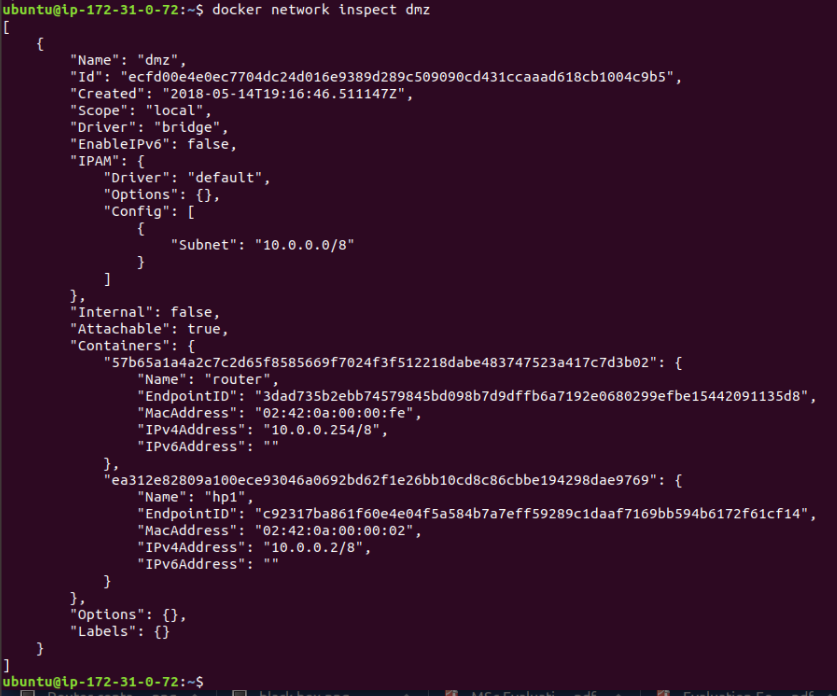
\includegraphics[width=160mm, scale=1]{Images/docker_network_inspect_dmz.PNG}
      \caption{Console Output of \textit{docker network inspect dmz}} 
      \medskip
      \small
		An image showing the console output obtained by executing the command \textit{docker network inspect dmz}. It can be observed that there are 2 containers on this network: The \textit{router} container, and the \textit{hp1} Cowrie container. 
\label{fig:docker-network-inspect-dmz}
\end{figure}


The correct routing of attack traffic from the \textit{router} container through the \textit{dmz} to the \textit{hp1} Cowrie container could be tested from inside the router container. Once inside the \textit{router} container, connecting over SSH or telnet to the \textit{hp1} honeypot and being presented with the Cowrie login prompt verifies the correct configuration of the network. Figure \ref{fig:cowrie-ssh-login-from-router} shows the console output when an SSH connection is attempted from the \textit{router} container to the \textit{hp1} container, demonstrating the correct routing of traffic within the \textit{dmz} network.

\begin{figure}[ht]
      \centering
      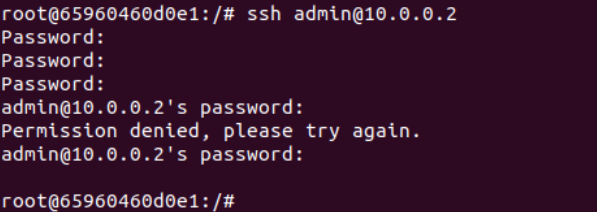
\includegraphics[width=160mm, scale=1]{Images/example-ssh-login-cowrie-container.PNG}
      \caption{A Denied SSH Login from the Router to a Cowrie Honeypot} 
      \medskip
      \small
		This screenshot shows a simulated attack session from the \textit{router }container to the \textit{hp1} Cowrie honeypot container. It can be observed that the ''attacker'' attempts to log in to  the \textit{hp1} container as user \textit{admin}. The first password provided for login is rejected, and a second prompt for the correct password is requested by the \textit{hp1} Cowrie honeypot. In this case, the attacker decides to cancel the login attempt rather than proceeding with a second login attempt.
\label{fig:cowrie-ssh-login-from-router}
\end{figure}

%\includewidefigure{cowrie-ssh-login-from-router}{A Denied SSH Login from the Router to a Cowrie Honeypot}{This screenshot shows a simulated attack session from the \textit{router }container to the \textit{hp1} Cowrie honeypot container. It can be observed that the ''attacker'' attempts to log in to  the \textit{hp1} container as user \textit{admin}. The first password provided for login is rejected, and a second prompt for the correct password is requested by the \textit{hp1} Cowrie honeypot. In this case, the attacker decides to cancel the login attempt rather than proceeding with a second login attempt.}{Images/example-ssh-login-cowrie-container.PNG}

    
%% 
%% SECTION 4: Visualisation
%%

\section{Visualisation of Attack Data} \label{LoggingAndVisualisationSection}
As decided in \textit{Section \ref{VisualisationDesignChoice}} as part of the design process, the data generated by honeypots in the Docker honeynet would be visualised using the ELK log processing stack on a separate EC2 server instance. The deployment of the EC2 management server instance was already described in \textit{Section \ref{DeployingTheManagementInstance}}, and this section details the installation and configuration of the tools on this instance to enable the processing and visualisation of the honeypot data.

\subsection{Management Server Instance}
The EC2 management server instance had already been deployed with sufficient hardware resources to meet the requirements of the ELK stack. Since the ELK stack is widely used for log processing and visualisation, there were plentiful resources available from which to learn, showing how to configure these open-source tools to work together.

Some complementary tools were also used in order to facilitate the use of the ELK stack for analysis of logs from a remote machine: In particular, Nginx and Filebeat. The configuration and interoperation of all of these tools is described in the following subsections.

	\subsubsection{Elasticsearch}
    Elasticsearch is an open-source search and analytics engine built on the Apache Lucene API. The fact that it supports analysis of JSON-formatted files made it an ideal choice for the analysis and indexing of the Cowrie logs, which are logged in JSON format.
    
    To set up the environment to run Elasticsearch, Java 8 was first required as a prerequisite installation. Once Java 8 has been installed, Elasticsearch was then also installed. Next, in order to configure Elasticsearch securely external access to the application needed to be restricted. This is important, since Elasticsearch provides a HTTP API that can be queried to perform manipulation on the data stored in the Elasticsearch index. If access to this was not restricted, the data in the index could be modified or removed without authorisation.
    
    By editing the \textit{/etc/elasticsearch/elasticsearch.yml} configuration file for Elasticsearch, external access was completely restricted by setting the access address \textit{network.host} to \textit{localhost}\footnote{The IP address 127.0.0.1 is known as the localhost address.}. This meant that Elasticsearch could only be accessed from the management instance itself on localhost, on the Elasticsearch default port 9200/TCP. 
    
	\subsubsection{Kibana}
    
    The Kibana visualisation engine was the second component of the ELK stack to be installed and configured. Kibana is an open-source analytics and visualisation platform, designed specifically to work with the Elasticsearch search platform. The use of Kibana in this project was intended to make analysis of the honeypot log files painless and immediate. 
    
    Kibana provides a web interface through which visualisations can be accessed. By configuring rules to visualise incoming log data, Kibana makes it possible to understand crucial information about the state of the system instantaneously.
    
    Similarly to Elasticsearch, it was important to set up Kibana to have restricted accessibility from external systems. In order to achieve this whilst still allowing an administrator to access the visualisations through the web interface, the Nginx reverse proxying tool was used.
    
		\subsubsection{Nginx}
        
Nginx is an open-source tool focused on providing services like web serving, reverse proxying, caching, and load balancing. \cite{Nginx} In this system, it was used to allow access to the Kibana web interface using reverse-proxying. 

An authentication step was configured with a single valid username-password credential to allow for authenticated login from a web browser. A small amount of additional configuration was then required to direct incoming HTTP traffic to the Kibana application\footnote{This involved the addition of the EC2 management server instance's public IP address to a Nginx  configuration file in the \textit{sites-available} directory.}.
      
	\subsubsection{Logstash}
    Logstash is an open-source log pipeline tool which accepts, processes, transforms and outputs data from log files provided to it, and was the final component configured on the management server instance. 
    
    As discussed in \textit{Section \ref{SecureLogTransfer}}, an SSL certificate was generated by using the private IP of the server in the SAN field. This would later be used by Logstash to verify the origin of log data shipped by Filebeat.
    
    %%Nice diagram: https://www.elastic.co/guide/en/logstash/2.4/advanced-pipeline.html
    In order to configure the processing components of Logstash, a number of configurations needed to be defined to deal with each of the incoming log formats: Input, filter and output configurations. These were all specified as part of the same file, \textit{03-cowrie.conf}. 
 \begin{itemize}
    \item \textbf{Input}
    
    Inputs are a field used to pass data into the Logstash pipeline. In this system, a single input was defined to accept data of type \textit{beats}, corresponding to data shipped by Filebeat. 

A port number was specified from which this data should be received by Filebeat. The path to the generated SSL certificate was also specified, so that the data received on this port could be verified by Logstash.
    \item \textbf{Filter}
    
    Filters are an intermediary processing step in the Logstash pipeline, where operations can be applied to the input data. An excellent tutorial was identified which explained a number of different filtering operations that could be applied to the Cowrie logs. These formed the basis of the filtering operations configured in this field\footnote{It should be noted that although substantial effort was expended to perform the similar filtering operations on the \textit{syslog} files generated by the router container honeypot, there were multiple compatibility issues encountered which resulted in the failure to visualise these logs on the Kibana web interface.}. \cite{FernandoDominiguezCowrieLogstashConfig}
    \item \textbf{Output}
    
    Outputs are last field in the Logstash processing pipeline, piping the results of the processing to a designated output process. In this case, the output process was Elasticsearch, which had been configured to listen for incoming data on localhost, port 9200. Some additional options were specified regarding the formatting of the data to be stored in the Elasticsearch index.
    \end{itemize}
    
    
\subsection{Honeypot Instance}
To provide the EC2 management instance with honeypot data to visualise, the logs generated by the honeypot containers on the EC2 honeypot instance needed to be aggregated and then transferred securely to the management instance. This was achieved as described below.

	\subsubsection{CRON \label{CRON}}
		
		A CRON job was configured to run every 60 seconds on the honeypot instance, shipping the honeypot logs from their respective container volumes to a defined location on the honeypot instance: The \textit{/var/logs/} directory. This meant that logs generated by all honeypots present would be aggregated in a single location on the honeypot instance.
        
\includecode{CRON Log Shipping Job}{This snippet shows 2 tasks scheduled using CRON, which copy the contents of the honeypot container volumes to the \textit{/var/logs} directory. These jobs are run every 60 seconds, the maximum possible frequency for a CRON job.}{Code_snippets/cron.txt}

	\subsubsection{Filebeat}
    Filebeat is an open-source application which was discussed in \textit{Section \ref{SecureLogTransfer}} in the context of securely transferring honeypot logs from the EC2 honeypot instance to the EC2 management instance using SSL certificates. The SSL certificate previously generated by the management server was shared with the honeypot instance using Secure Copy (SCP).
        
    The Filebeat configuration file, \textit{/etc/filebeat/filebeat.yml}, was configured to inspect the \textit{/var/log} directory on the EC2 honeypot instance for the presence of log files any time updated log files were added to it by CRON. It was then configured to send the logs to the EC2 management instance using private IP addressing, specifying the destination port to be the same as that configured in the \textit{input} field of the Logstash configuration file. Lastly, Filebeat was configured to use the SSL certificate generated by the EC2 management instance for all data transferred.


\section{Alert/Notification System}\label{AlertSystemSection}
As another important element of the cyber incident monitor identified in \textit{Section \ref{IncidentMonitoringDesign}}, the configuration of a threat notification system was the final step in the implementation of the cyber incident monitor.

\subsection{PSAD}
As explained in \textit{Section \ref{DesignChoicePSAD}}, PSAD was identified as the tool of choice to enable alerting of system administrators to potential attacks happening on the honeypot host. It was deployed on the honeypot instance in order to provide an instantaneous notification to system administrators of potential attacks. A basic configuration generated email alerts when probing of the honeypot instance was detected, sending notification emails to the address \textit{itsmyjobtofixtheproblem@outlook.com}, which could be specified in the \textit{/etc/psad/psad.conf} configuration file. It was possible to configure PSAD to check the state of the network event logs as frequently as desired, for which a reasonable frequency was chosen to be every 5 seconds.

\begin{figure}[ht]
      \centering
      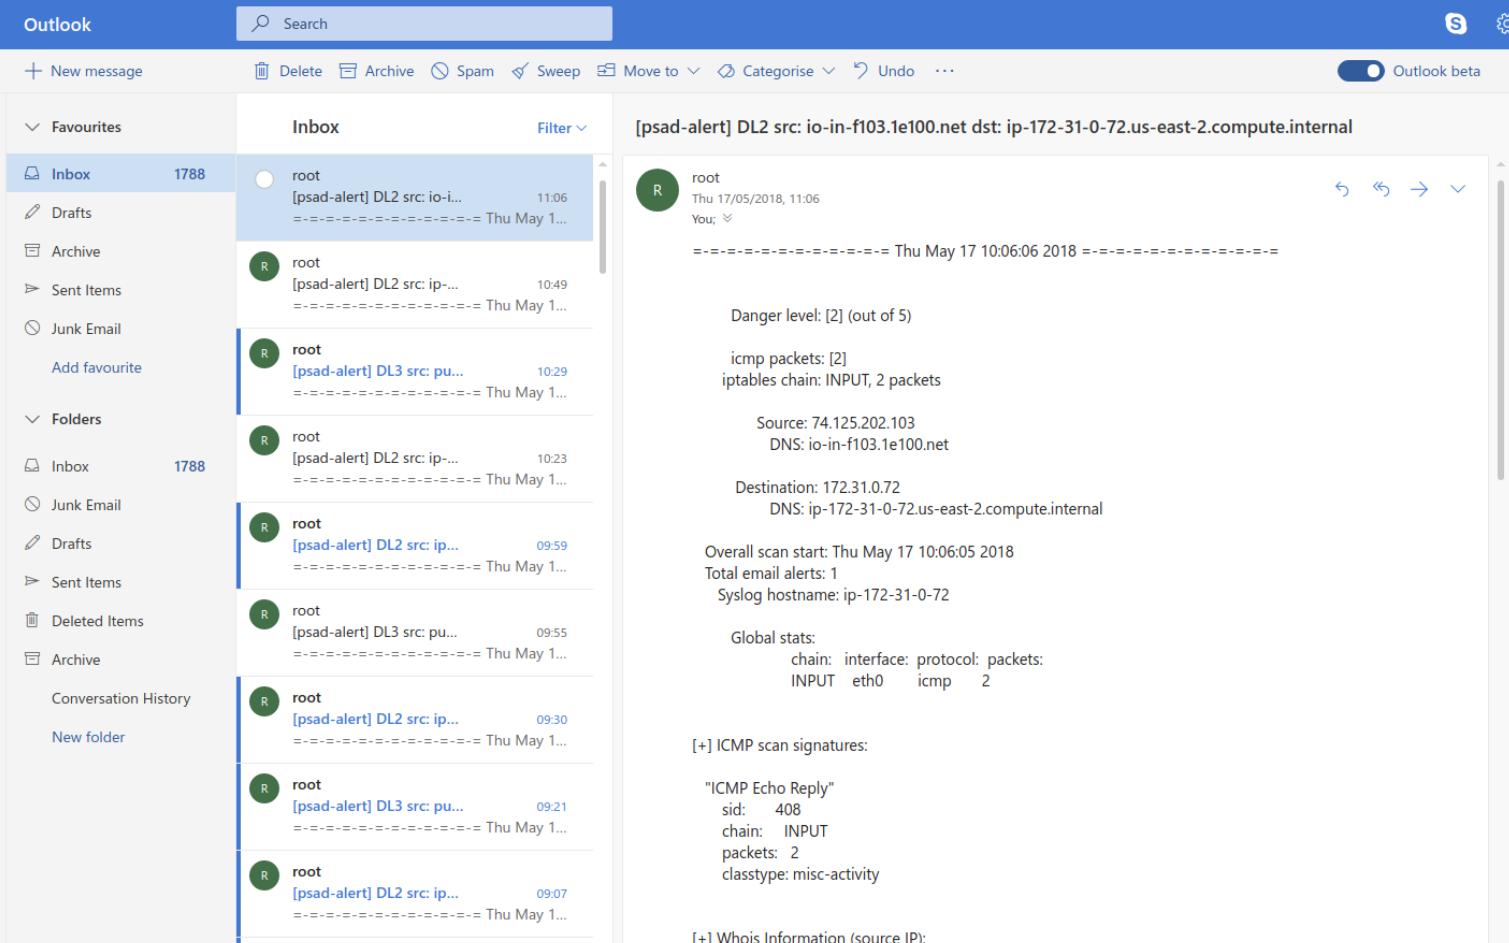
\includegraphics[width=160mm, scale=1]{Images/psad-email-alert.PNG}
      \caption{An Email Alert from PSAD} 
      \medskip
      \small
		This screenshot shows the email inbox to which PSAD was configured to send email alerts. It can be seen that a port scan generated an email alert shown in the right-hand pane of the email inbox. PSAD has detected that the source of the scan is a domain \textit{io-in-f103.1e100.net} which has sent a number of ICMP packets to the EC2 server instance, triggering this alert.
\label{fig:psad-email-alert}
\end{figure}

With PSAD it is also possible to completely blacklist or whitelist\footnote{Whitelisting an IP address means that it is added to a list of addresses that are considered trustworthy.} certain IP addresses by editing the \textit{/etc/psad/auto\_dl} configuration file. This functionality was used to reduce the number of false positives being generated by PSAD\footnote{After PSAD was initially configured, there were many email alerts generated from a particular server called \textit{chillipepper.canonical.com}. Upon contacting Canonical Ltd. about the possibility of their server being compromised and used to launch attacks, it was found that the alerts were being generated by benign Network Time Protocol (NTP) time synchronisation traffic.}.

\section{Summary \label{ImplementationSummary}}
By the time all of the system components had been configured and implemented as described in this chapter, an end-to-end system cyber incident monitoring system was in place.

\begin{itemize}
\item Attack sessions could be simulated, connecting to the EC2 honeypot instance over SSH or telnet and being presented with the router container login prompt. After authenticating with the router container, it was possible to connect in the same way to any container in the honeynet and interact with a Cowrie honeypot.
\item All activity generated from interactions with the Cowrie containers was being successfully shipped, processed and visualised, with the visualisation dashboard accessible from a web browser.
\item The entire Docker environment could be completely removed and redeployed with an identical configuration if required.
\end{itemize} 

Thus, the objective of developing a honeypot-driven cyber incident monitor had largely been achieved at this point, with much remaining scope for configuration of both the honeypots and the visualisations once attack data had been obtained. This system would be used to conduct a series of experiments focused on determining effective design for adaptive honeypots, detailed in \textit{Chapter 6}.				%% IMPLEMENTATION


\chapter{Evaluation} \label{Chapter6}

%; including, but not limited to, machine type advertised, publicly open ports, running processes etc.
This chapter focuses on providing an evaluation of the implemented cyber incident monitoring system, as well describing the design and conducting of experiments as part of the proposal for adaptive honeypot design.

\textit{Section \ref{DesignOfExperiments}} provides an in-depth explanation of how the experiments were designed for evaluating the impact of attractiveness honeypot characteristics on the number of attacks received.

\textit{Section \ref{ConductingExperiments}} discusses how the experiments were conducted and their limited findings, detailing the nature of numerous setbacks that occurred and how these were dealt with. An explanation for the early conclusion of these experiments is also provided.

\textit{Section \ref{DiscussionOfEvaluation}} discusses the limited findings of the experiments as well as a qualitative evaluation of the cyber incident monitoring solution produced.

Finally, \textit{Section \ref{SummaryOfChapter6}} provides some brief conclusions regarding the evaluation of the honeypot experiments.

\section{Design of Experiments \label{DesignOfExperiments}}
The conducting of experiments in this research is focused on the delivery of the second objective outlined in \textit{Section \ref{Objective2}}: To determine an improved design for effective, adaptive honeypots. It was decided that the measure of effectiveness in these experiments would be defined by how many attacks each honeypot received. From this, it would be possible to present findings and draw conclusions regarding the development of effective adaptive honeypots. 

The design of the experiments was influenced greatly by the time that remained to complete the entirety of the research: A period of just four weeks. A series of experiment iterations were devised to be run over the course of these 4 weeks. Table \ref{table:HoneypotExperimentsTable} describes the variables involved in each iteration, and the intended execution of these iterations with respect to time. 


\begin{table}[!h]
\begin{center}
\begin{tabular}{|*{17}{c|}}  % repeats {c|} 17 times
\hline
\multicolumn{1}{|c}{} & \multicolumn{4}{|c|}{\textbf{Vendor A}} & \multicolumn{4}{|c|}{\textbf{Vendor B}} & \multicolumn{4}{|c|}{\textbf{Vendor C}} & \multicolumn{4}{|c|}{\textbf{Control}} \\ \hline
\multicolumn{1}{|c}{} &
\multicolumn{4}{|c}{\textit{Week 1}} & \multicolumn{4}{|c}{\textit{Week 2}} & \multicolumn{4}{|c}{\textit{Week 3}} & \multicolumn{4}{|c|}{\textit{Week 4}} \\ \hline 
 & \textbf{LC} & \textbf{SA} & \textbf{DT} &  & \textbf{LC} &\textbf{SA} & \textbf{DT} &  &\textbf{LC} & \textbf{SA} & \textbf{DT} & & \textbf{LC} &\textbf{SA} & \textbf{DT} & \\ \hline
\textbf{HP1} & A & X & P &  & A &X & P &  &A & X & P & &A & X &P &  \\ \hline
\textbf{HP2} & B & Y & Q &  & B &Y & Q &  &B & Y & Q & &B & Y &Q &  \\ \hline
\textbf{...} & C & Z & R &  & C &Z & R &  &C & Z & R & &C & Z &R &  \\ \hline
\textbf{HPN} & D & W & S &  & D &W & S &  &D & W & S & &D & W &S &  \\ \hline
\textbf{Control} & * & * & * &  & * &* & * &  &* & * & * & &* & * &* &  \\ \hline
 \end{tabular}
\end{center}
 \caption[Planned Iterations of the Honeypot Experiments]{A set of planned experiment iterations in order to propose an optimal honeypot design. Three characteristics of the N Cowrie honeypots HP1, HP2 ... HPN are considered: The login credentials accepted (\textit{LC}), the services advertised to be running on the container (\textit{SA}), and the type of device advertised (\textit{DT}). For each week, only one characteristic of the router honeypot is varied: The device vendor, corresponding to columns \textit{Model A, Model B,} etc. Each variation of a Cowrie honeypot characteristic (\textit{LC, SA, DT}) should be in place for 2 days, with all 12 experiment iterations taking place over 4 weeks. There is one day allocated per 7-day week for setting up the experiments, represented by the empty column for each week. In each iteration there is a single \textit{Control} Cowrie honeypot used as an indication of baseline performance, and in \textit{Week 4} a \textit{Control} router honeypot is also employed for the same reason.}	
\label{table:HoneypotExperimentsTable}
\end{table}

An explanation of how this plan translates into the configuration of the research environment is explained in the following subsections.

\subsection{Router Honeypot Container}
As the gateway between the public internet and the Cowrie honeynet, it is obvious that the router container should aid an attacker in accessing the deployed system. Facilitating easy access to this container is likely to increase the chance of a successful venture into the Cowrie honeynet, enabling valuable data to be captured. Thus, it was important to configure the router container to be as attractive and open as possible to the targeted attackers, IoT botnets. 

The system had already been designed and implemented to facilitate exactly these requirements, and so the router container could easily provide:

\begin{itemize}
\item Remote access over either SSH or telnet from the public internet;
\item Authentication using a number of valid username-password combinations;
\item Root privileges inside the system;
\item A powerful OS and toolkits;
\item A network of nearby hosts to which an attack could be propagated;
\item An attractive device banner indicating a device type.
\end{itemize}

In order to gain some insights regarding honeypot design from the router container  and not just from the Cowrie honeypots, it was decided to vary a characteristic of the router container honeypot as part of the experiments: The device vendor advertised\footnote{In order to facilitate easy access to the Cowrie honeynet whilst also gaining some insights from allowing attackers to access the router container, the device vendor advertised in the SSH and telnet banners of the router honeypot was deemed to be a suitable and useful characteristic to measure. If this characteristic was found to impact upon the number of attacks received, it would give an indication of vendor awareness in IoT botnets.}. All other characteristics of the router container would be held constant, such that the same username-password credentials, services, toolkits, etc. would be available on this honeypot in all experiment iterations. 

% over a number of iterations of experiments, one characteristic of the router container would be varied: 


With reference to the experiment iterations plan in table \ref{table:HoneypotExperimentsTable}, the following experiments were designed for the measurement of the impact of device vendor on the number of attacks received:

\begin{itemize}
\item For each of \textit{Week 1}, \textit{Week 2} and \textit{Week 3} shown in the table, the router container would be configured to advertise a different brand of router to through SSH and telnet banners. Each banner will be left on the router container for 6 consecutive days of that week, with every other variable in the router honeypot environment being held constant.
\item In \textit{Week 4}, a \textit{Control} router container would be used: One which doesn't advertise any brand or model, but which simply uses the default 'Ubuntu 16.0.4 LTS' SSH and telnet banner with hostname \textit{router}. By having a control, it is possible to compare the results of the other three weeks against a baseline to determine whether or not it matters that a device is advertised as being from a particular vendor.
\end{itemize}

For the 3 device banners to be configured on this honeypot for \textit{Week 1}, \textit{Week 2} and \textit{Week 3}, it is desirable to base those device brands used in the banner configuration on real-world data. Masscan is a powerful asynchronous port scanner which was used by the researchers behind the IoTPot honeypot to capture device banners from devices on the public internet listening on the telnet 23/TCP port. \cite{IoTPot2016} The researchers used these banners to customise the honeypots to look like a real telnet-enabled device on the Internet. The effectiveness of this approach in their evaluation of IoT botnet behaviour motivated the decision to use Masscan to capture device banners in this research for use in the experiments. The most commonly occurring device vendor banners would be used as a basis for the experiments, since a more popular device vendor can be assumed to be more likely to be attacked than a less popular one.

%After the end of the first week, I will change the brand/model of the router advertised - e.g. Netgear, Cisco, etc. depending on the most common banners from the masscan data. I will repeat the same experiments as before for the cowrie honeynet however, in order to ensure that I can clearly attribute any trends to a particular variation in a single parameter.


\subsection{Cowrie Honeypot Containers}
In the Cowrie honeynet, there is substantially more scope for measuring the impact of varying honeypot characteristics since there are a greater number of honeypots available: As motivated in the formulation of the research objectives in \textit{Section \ref{BenefitsForUsingHoneynetForExperiments}}, a honeynet provides a solution to the accurate measurement of relative effectiveness of honeypots in the same environment, since the effects of time can be largely disregarded\footnote{Since all honeypots in the honeynet should be simultaneously exposed to the same environmental conditions, the effect of time variability in the experiments is minimised.}.
% * <rohiggin@tcd.ie> 2018-05-16T14:01:08.245Z:
% 
% > \textit{Section \ref{BenefitsOfUsingHoneynetsForExperiment}},
% Add correct Section, comes up as "??"
% 
% ^.

For each of the 4 weeks for which the experiments would be run, it was decided that 3 honeypot characteristics would be varied for a period of 2 days per week each. These characteristics are:


\begin{enumerate}
\item The login credentials accepted by the honeypot;
\item The services running on the honeypot's container ports\footnote{In the research conducted by Dowling \textit{et al.} in the implementation of a Zigbee honeypot, the generation of unencrypted network traffic was an interesting honeypot characteristic used in an attempt to attract the attention of attackers. \cite{Dowling2017} Measuring the impact that such a measure has on the number of attacks received by a honeypot was deemed a useful characteristic to measure.};
\item The type of device advertised by the honeypot.
\end{enumerate}

To illustrate how this translates into an experiment iteration, consider column \textit{LC} in \textit{Week 1} in table \textit{\ref{table:HoneypotExperimentsTable}} as an example.
\begin{itemize}
\item \textit{LC} corresponds to the variation of the \textit{login credentials} accepted by honeypots HP1, HP2, ... HPN over a 2-day period.
\item For each of honeypots HP1, HP2, ... HPN, the login credentials accepted should vary. Other variabls should be held constant\footnote{This means that if the \textit{login credentials} (\textit{LC}) are the characteristic being varied, both the \textit{services advertised} (\textit{SA}) and the \textit{device type} (\textit{DT}) should be held constant}.
\end{itemize}

It was decided that five Cowrie honeypots would be deployed in each experiment iteration, one of which would be the control honeypot. The presence of a control iteration is important, since it allows for definitive conclusions to be drawn as to whether or not the results obtained by customised honeypots have any impact on the number of attacks they receive. 

% Wikipedia definition of experiment control: designed to minimize the effects of variables other than the independent variable. This increases the reliability of the results, often through a comparison between control measurements and the other measurements.

 
%
%	SECTION 2: CONDUCTING EXPERIMENTS
%
 

 \section{Conducting Experiments} \label{ConductingExperiments}
The experiment iterations were planned to be conducted in the order in which they are specified in table \ref{table:HoneypotExperimentsTable}, starting with varying the login credentials of the Cowrie honeypots and the addition of a banner advertising a device manufacturer.


\subsection{Capturing Device Banners}
Masscan was used to scan the entire IPv4 address space for devices listening on ports 22/TCP (SSH) or 23/TCP (telnet) over the course of two days. The telnet and SSH banners of any device that responded were captured in log files. The IP addresses of these devices were also captured.

The banners were extracted from the log files into a new file, where they were counted using shell commands. In total, 71,149 banners were captured after scanning port 23/TCP (telnet) and 179,849 banners were captured after scanning port 22/TCP (SSH). 

Many of the banners obtained specified vague information regarding device models and manufacturers, with many not being identifiable from the device banners at all. In order to make the results obtained relatively usable for falsifying honeypot device banners, the Masscan results were used in conjunction with Google searches to identify vulnerable device models.

\subsection{Experiment 1, Attempt 1}
The first experiment iteration undertaken corresponds to the \textit{Week 1, LC} experiment shown in table \ref{table:HoneypotExperimentsTable}. This involved the variation of login credentials accepted by the Cowrie honeypots deployed in the Docker honeynet, and the configuration of a vendor-specific device banner on the router container.


\subsubsection{Configuration of the Router Honeypot}
Huawei devices were encountered 42 times explicitly in telnet banners, and 6 times explicitly in SSH banners\footnote{It is assumed that not all Huawei devices scanned will have provided an explicit Huawei banner in response to the Masscan probes. Thus, there could have been many more Huawei devices present in the results found which could not be identified simply from their banners. }. This made Huawei the most popular router manufacturer that could be identified from the captured banners. However, since no discernible models could be identified from these banners some research was conducted into vulnerable Huawei router models, immediately identifying their HG-532d model as being highly vulnerable to exploit. \cite{HuaweiHG532dVulnerabilityAdvisory} \cite{CheckpointHuaweiHG532dVulnerability} The device manual was found to contain the default username-password credentials \textit{user/user}. Thus for this experiment iteration, the router container was advertised as a Huawei HG-532d router. 

In order to facilitate as many successful logins as possible, the router container was configured to allow passwordless login for 14 different user accounts. These user accounts were added based on results captured from a temporary deployment of a plain Cowrie honeypot on an AWS EC2 instance, which was set up to capture credentials that are actually being used by IoT botnets for brute-force authentication\footnote{The full list of user accounts added were \textit{root}, \textit{admin}, \textit{cisco}, \textit{guest}, \textit{admin1}, \textit{support}, \textit{ubnt}, \textit{default}, \textit{Admin}, \textit{service}, \textit{supervisor}, \textit{Administrator}, \textit{administrator}, and \textit{user}. There were also a number of additional usernames captured: However, these contained numbers which are invalid characters for Ubuntu usernames, meaning that they could not be added as an user. The \textit{user} username was added based on the fact that the Huawei HG532d device manual specified this as the default username.}. 

\subsubsection{Configuration of the Cowrie Honeypots}
As discussed, five Cowrie honeypots were deployed as part of this experiment iteration. One of these honeypots was the control, a plain Cowrie honeypot with no customisations added to it.

Since the login credentials were the characteristic being varied across the remaining 4 honeypots in this experiment iteration, the device type and services available on the honeypots needed to be kept constant.

\begin{itemize}
\item \textbf{Device Type Advertised}

All honeypots were given device names similar to the default hostname assigned to Cowrie. Thus the Cowrie honeypots were named \textit{srv01}, \textit{srv02}, \textit{srv03}, \textit{srv04} and \textit{srv05}, where \textit{srv04} was the \textit{control} honeypot.

\item \textbf{Services Advertised}

The simplest solution to keeping the services advertised by the honeypots constant was to use the default Cowrie container configuration, where the emulated SSH and telnet services were the only services that would be detected by an attacker performing a port scan on these honeypots.

\item \textbf{Login Credentials Accepted}

Different accepted login credentials were configured on each of the Cowrie honeypots, with the exception of the control honeypot \textit{srv04}. These were as follows:
    \begin{enumerate}
        \item \textit{srv01} accepted username \textit{root} with any password;
        \item \textit{srv02} accepted username \textit{admin} with any password;
        \item \textit{srv03} accepted any credentials provided after a random number of attempts, which can be configured using the Cowrie's \textit{AuthRandom} option\footnote{By setting this option in the \textit{cowrie.cfg} file, access will be granted to an attacker after \textit{randint(minimum, maximum, cache\_combinations)} login attempts. In this case the parameters specified were 3, 5 and 10 respectively.} in the \textit{cowrie.cfg} file;
 		\item \textit{srv05} used the username-password combinations captured from one of the four attackers in the first exposure of Cowrie to attack\footnote{All of the brute-force login attempts from this bot used the username \textit{admin}, along with a total of 13 different passwords.}, explained in \textit{Section \ref{ExposingCowrieToAttack}};

\end{enumerate}
\end{itemize}

\subsubsection{Findings of the Experiment}
Once the system was exposed to the public internet on ports 22/TCP (SSH) and 23/TCP (telnet), there were immediately plenty of connection attempts captured by the router container over both SSH and telnet. However, it was soon observed based on the event timestamps that most connections were terminated immediately after connecting. 

It was concluded upon reflection that this behaviour could be due to detection of the system as a honeypot environment: Since attackers were being given passwordless root access to the router container, it would be reasonable to expect this to raise suspicions about the legitimacy of the system. This is not ideal, since the intention behind allowing passwordless access was to enable attackers to easily gain access to the system: The addition of password authentication, which allows only 1 password per system user, would restrict the number of attackers that could successfully access the system.

The experiment iteration was concluded after 2 days. By this time, there were no attacks logged by any of the Cowrie honeypots in the honeynet, since no attackers had progressed beyond the router container. It was decided on this basis that the experiment iteration should be repeated under the same conditions, with the exception that passwordless access to the router container should no longer be provided.

\subsection{Experiment 1, Attempt 2}
Based on the failure of the system to capture any substantial attack data in the first attempt of experiment iteration 1, the system was re-deployed with the same configuration. This time however, passwordless authentication to the router container would not be permitted.

\subsubsection{Reconfiguring the Router Credentials}
As an alternative to passwordless authentication, it was decided that the password for each existing user account would be configured to be identical to the username for simplicity: For instance, for user \textit{admin} the password would also be \textit{admin}. This seemed a reasonable choice for permitted login credentials for each user account on the router container, since identical username-password combinations are commonly used in brute-force authentication attacks.

Adding this involved some simple edits to the router container's entrypoint script.

\subsubsection{Findings of the Experiment}
\label{Experiment1Iteration2Results} It was discovered after less than 24 hours of running this experiment that the EC2 honeypot server instance had completely crashed. Upon investigation, this crash appeared to be due to an unusual \textit{fork bomb}\footnote{A fork bomb is an unintended behaviour of a system, where processes are continually made to replicate themselves until all available CPU resources are depleted, resulting in a crash failure of the system. It is often used as a DOS attack.} behaviour by CRON: The \textit{syslogs} showed that it had recursively restarted itself until there were too many processes for the EC2 host to handle, eventually crashing the instance entirely.

After checking the logs generated by the router container, there were a number of successful connection sessions logged for both SSH and telnet: However, after examining the \textit{.bash\_history} file none of the commands executed looked like they could have caused this fork bomb behaviour to occur intentionally. It was thus concluded that this had occurred due to a resource overload on the system

Though the system had been offline for quite some time before the failure was discovered, in the few hours that the experiment had been running there had been a number of successful login attempts to the router container. However, there were also no attacks that had reached the Cowrie honeynet. 

The contents of the \textit{.bash\_history} file showed only 6 commands had been executed during the time that the experiment was running. Three similar sequences of commands had been executed as follows:

\begin{center}
    \textit{cat /proc/mounts; (/bin/busybox LWQTL || :)}
    
    \textit{cd /dev/shm; cat .s || cp /bin/echo .s; (/bin/busybox LWQTL || :)}
    
    \textit{cat /proc/mounts; (/bin/busybox GQZJN || :)}
    
    \textit{cd /dev/shm; cat .s || cp /bin/echo .s; (/bin/busybox GQZJN || :)}
    
    \textit{cat /proc/mounts; (/bin/busybox WEGOD || :)}
    
    \textit{cd /dev/shm; cat .s || cp /bin/echo .s; (/bin/busybox WEGOD || :)}
\end{center}


Of note was the fact that these commands attempted to invoke the \textit{BusyBox} shell, which had not been installed in the router container as an oversight in the implementation process. In their analysis of the behaviour of the Hajime IoT botnet, Edwards \textit{et al.} noted almost identical invocations of the \textit{BusyBox} shell as part of what they deduced was a fingerprinting mechanism to determine the properties of the victim system. \cite{HajimeMysteriousBotnet} A legitimate system on which BusyBox had been installed would return the response \textit{'CHDGL: applet not found'}. Also noted by these researchers is the purpose of the \textit{cat /proc/mounts} command sequence which ''checks the system mounts for a writeable location in the target filesystem'', and the sequence \textit{cd /var; cat .s || cp /bin/echo .s; /bin/busybox ECCHI}, which among other things ''picks the first writeable path that is not /proc, /sys, or / and uses that as its working path''. The fact that these commands were observed may indicate the presence of the Hajime botnet.

Overall, the results of this experiment iteration were interesting but not complete, since no attacker progressed beyond the initial fingerprinting stage because of the absence of the \textit{BusyBox} utility. It would be necessary to run this experiment iteration a third time with the utility installed.

\subsection{Experiment 1, Attempt 3}
The same experiment that was set up in the previous two iterations was re-deployed for a third time after adding the \textit{BusyBox} utility to the router container Dockerfile. There was no additional configuration of this utility required, and it was simply installed upon rebuilding the container image.

\subsubsection{Findings of the Experiment}
As planned, the experiment iteration was run for two days before the system was taken offline and the results examined. This time, the network events logged by \textit{syslog} showed that several more attackers had managed to successfully authenticate with the router container over both SSH and telnet.

The environment was examined, and the findings were as follows:
\begin{itemize}
\item Even after repeating this experiment for a third time, no attacker had proceeded from the router container to the Cowrie honeynet. This was evident from the fact that there were no Cowrie visualisations generated on the Kibana dashboard hosted by the management server. There were also no commands observed in the \textit{.bash\_history} file that would indicate an attacker having probed the \textit{dmz} network.
\item Like the previous iteration, commands were observed in the \textit{.bash\_history} file that could be attributed to bot attackers. However, only one sequence similar to those highlighted in \textit{Section \ref{Experiment1Iteration2Results}} was observed. Instead, another sequence \textit{enable;  system;  shell;  sh} was repeatedly observed. This was another sequence discussed by Edwards \textit{et al.}, which they explain ''are sent in a blind attempt to navigate whatever vendor-specific command-line interface (CLI) the Telnet server implements.... If any command fails, it will fail''. \cite{HajimeMysteriousBotnet} Upon manually attempting to execute the same sequence inside the router container, it was found that the \textit{system} and \textit{shell} commands did not execute inside the container, explaining the fact that the attack sequence ended at this point.
\item It appeared that a human attacker had gained access to the system in this experiment\footnote{This was inferred by the commands that were found to have been executed after inspecting the \textit{.bash\_history} file, in particular the \textit{clear} command which is used to clear the output displayed in a Linux console window. This is a command that would be useless to an automated bot attacker, and was a tell-tale sign of a human attacker.}. The \textit{.bash\_history}, when examined, showed that the attacker had downloaded a Python script from a web domain\footnote{The URL from which this script was downloaded is http://cybernetik.000webhostapp.com/speedtestvps.py. At the time of writing, the site hosted at this address had been taken down: However, a screenshot of the domain landing page captured after discovering this activity can be seen in figure \ref{fig:CyberMafiaDDoSForHire}. } after installing the \textit{wget} utility. Upon visiting this domain, the script was found to contain open-source licensing information, and was traced back to an open-source Github project called \textit{speedtest-cli}. \cite{SpeedtestCLITool} This is a tool used to test the network bandwidth available to a device, something that is undoubtedly of interest to an attacker intending to conduct a volumetric network attack such as DDoS. Other activities within the same session included the creation of a new user \textit{huawei}, checking the uptime of the system using the \textit{uptime} command, and checking the system specifications using the \textit{lscpu} command.
\end{itemize}

\begin{figure}[ht]
      \centering
      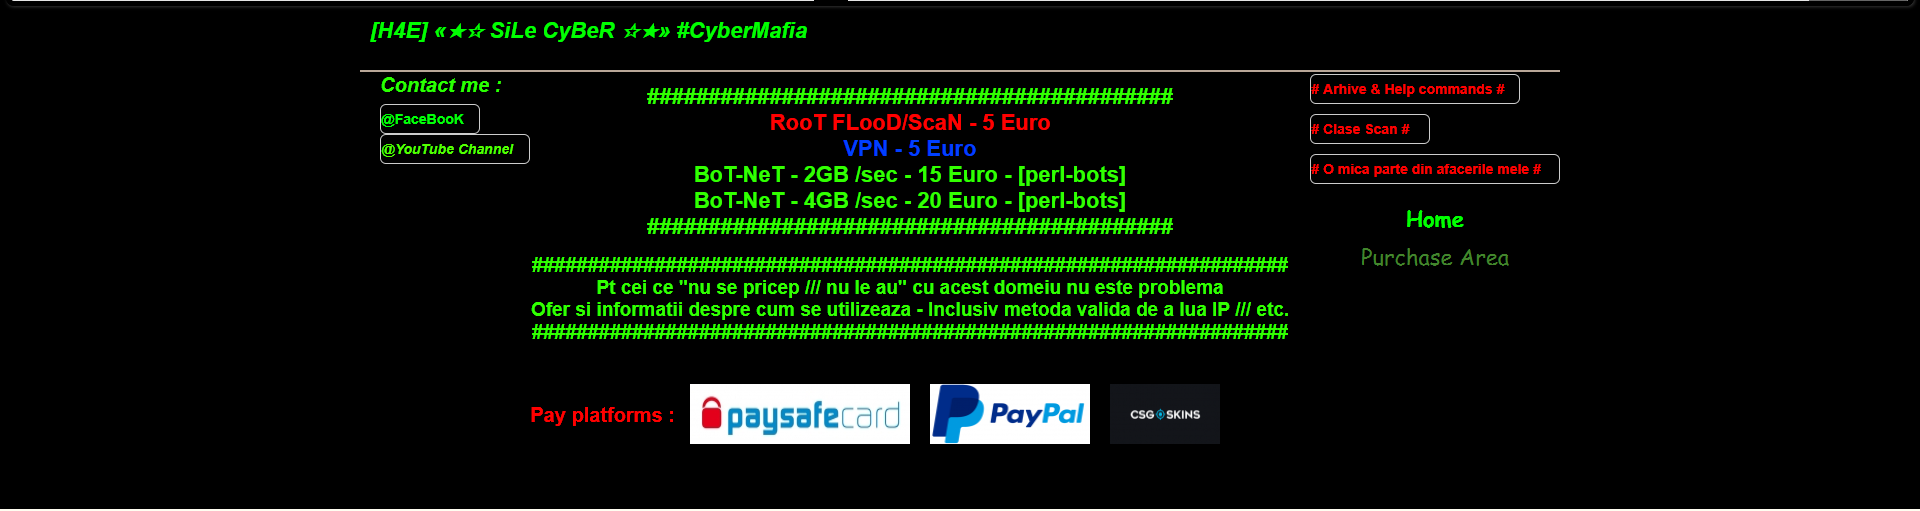
\includegraphics[width=160mm, scale=1]{Images/cybermafia_ddos-for-hire.PNG}
      \caption{DDoS-for-Hire: The Web Domain of a Human Attacker} 
      \medskip
      \small
		The webpage shown was linked to an attack session in the router container honeypot, where a Python script was downloaded from this site and used to measure the network bandwidth available to the system. The homepage shown in this image advertises DDoS-for-hire services, where it costs  \euro{15} to buy a 2GB/second attack and a 4GB/second attack costs \euro{20}.
\label{fig:CyberMafiaDDoSForHire}
\end{figure}
 
%\includewidefigure{CyberMafiaDDoSForHire}{DDoS-for-Hire: The Web Domain of a Human Attacker}{The webpage shown was linked to an attack session in the router container honeypot, where a Python script was downloaded from this site and used to measure the network bandwidth available to the system. The homepage shown in this image advertises DDoS-for-hire services, where it costs  \euro{15} to buy a 2GB/second attack and a 4GB/second attack costs \euro{20}.}{Images/cybermafia_ddos-for-hire.PNG}


\subsection{Concluding the Honeypot Experiments}
Something that became very clear from the experiments conducted was the unpredictability of conducting honeypot experiments. Given that 4 weeks had been allocated to complete all 12 iterations of experiments planned, it was crucial that there were minimal setbacks to the progression of the experiments within this time.

Over a week after setting up the first of these 12 iterations, the first experiment iteration had been deployed a total of three times due to the issues outlined in \textit{Section \ref{ConductingExperiments}}. It was concluded that conducting the remainder of the planned experiments was infeasible, given that less than three weeks remained to conduct the remaining iterations. Thus, the conducting of the planned experiments was discontinued.



%
%	SECTION 3: DISCUSSION
%


\section{Discussion} \label{DiscussionOfEvaluation}
% Will be more qualitative than quantitative.
Both the achievements and the limitations of the research are evaluated and discussed in this section. 

\subsection{Honeypot-Driven Cyber Incident Monitoring}
The first objective of this research was to develop a honeypot-driven cyber incident monitor that would be feasible to deploy in modern IT infrastructures, making it feasible for organisations to implement active network defence.

\subsubsection{Effectiveness of  the Containerised Honeynet}
% Piscarcik refer to the same paper:  scalability, flexibility, compromise, non-detectability and ease of deployment are key requirements for such a system.
As one of the novel features of the implemented incident monitoring system, the effectiveness of the honeynet deployment proposed by this research forms an important component of the evaluation. A useful set of criteria outlined by Chin \textit{et al.} \cite{5319295} and used by Piscarcik \textit{et al.} \cite{Pisarcik:2014:FDV:2659651.2659685} to evaluate their honeynet deployments specifies a number of key criteria that should be fulfilled by an effective honeynet. These are discussed below in relation to the system implemented in this research.

\begin{enumerate}
\item \textbf{Scalability}

The proposed solution is scalable insofar as it has been tested. The largest honeynet deployment trialled during the research consisted of 11 containerised honeypots\footnote{10 Cowrie honeypot containers and the router honeypot container.}, which was hosted continuously for 2 days without any component failing. However, during this period there was very little interaction with the system, limiting the load on system resources that would be present in a production environment.

In theory, the honeynet is capable of supporting a large number of honeypot containers. The ability to add more honeypots is largely dependent on the system resources available: The host system must have sufficient resources to support the number of containers  deployed. This is however certain to be much less than that required for an equivalent number of virtual machines on the same host.
 
\item \textbf{Flexibility} 

The implemented honeynet solution is flexible in its operability, configurability and maintainability. 
\begin{itemize}
\item Control over the honeynet from an administrative perspective is straight-forward: Containers can be managed through the host even whilst running, meaning that reconfiguration of the networking and administrative access to container resources can be done on-the-fly as required.
\item The use of the Cowrie honeypot also contributes to the flexibility of the honeynet. As a highly configurable and customisable open-source honeypot, tweaking the configuration of the honeypots in response to new threat insights is very achievable. 
\item It would also be relatively straight-forward to use a different honeypot in place of Cowrie in this system: Without having to make any changes to the network configuration, new Dockerfiles can be defined for alternative honeypots if required, integrated to the system with simple edits to the deployment script.

\end{itemize}
\item \textbf{Attack Containment}

Attack containment refers to the restriction of propagation of attacks if a honeypot is compromised. Though attack containment is never completely assured, the measures taken to provide attack containment described in \textit{Section \ref{DockerSecurityConsiderations}} mitigate against undesirable attack propagation outside the honeynet.
\begin{itemize}
\item The isolation of the host from the \textit{dmz} network on which the honeynet is hosted restricts the ability of an attacker to launch a network-based attack from within the honeynet. 
\item The carefully considered restrictions placed on an attacker inside the Cowrie honeypots mean that it is highly improbable that an attacker would be able to launch an attack from these honeypots in the first place. The fact that the Cowrie honeypot is an emulated environment in particular restricts an attackers activities, since they are not interacting with a real system with a networking stack, OS and powerful utilities.
\item The high-interaction router container is the only component of the system where attack containment may not be fully assured, since this container interfaces directly with a network to which the host is connected. This is a potential area for improvement, where given additional time investigating the use of alternative networks that don't interface with the host system could yield an improved level of isolation.
\end{itemize}
\item \textbf{Stealth}

Stealth refers to the ability of the honeynet to deceive an attacker and convince them that it is a legitimate system. It is difficult to provide a definitive conclusion regarding this property of the deployed honeynet, given that the interactions of attackers with the system were limited at best. 

There is certainly scope for improvement of the stealth of the honeynet based on the little data that was obtained through the experiments outlined in \textit{Section \ref{ConductingExperiments}}, since in each iteration it was found that IoT bot attackers did not progress their attacks beyond their known initial phases. \cite{UnderstandingTheMiraiBotnet} \cite{HajimeMysteriousBotnet}  To reach any definitive conclusions about this property would require substantially more time and experimentation.

However, the properties of the containerised honeynet lend themselves to deceiving attackers about the legitimacy of the environment, since all honeypots are hosted in containers with real OS images and networking stacks. For instance, Chin \textit{et al.} propose that stealth can be achieved through measures such as falsifying high network latency. \cite{5319295} An attacker testing the legitimacy of this honeynet based on such properties will receive legitimately delayed responses by virtue of the use of containers in the system.

\item \textbf{Resource Management} 

This criterion refers to the presence of simple mechanisms for allocating resources in the honeynet, which is largely provided through the use of Docker in this implementation. 
\begin{itemize}
\item The nature of containers is that the resources allocated to the running of an application are highly controlled and specified entirely by their image definition. In order to allocate additional resources, a simple update to this image definition is all that is required.
\item The host system resources consumed by containers are controllable primarily through the specification of arguments when creating containers. As stated in the Docker documentation, ''by default, a container has no resource constraints ... Docker provides ways to control how much memory, CPU, or block IO a container can use, setting runtime configuration flags of the docker run command''. \cite{DockerResourceConstraints} Though these resource restrictions were not explicitly addressed as part of the development of the containerised honeynet, it would be straight-forward to add these resource restrictions to the deployment script as part of  the \textit{docker create} commands.
\end{itemize}


\item \textbf{Ease of Deployment} 

Chin \textit{et al.} state that for a honeynet to be considered easy to deploy, ''users are not burdened by complicated configurations and procedures in order to set up their own honeypots''. 

In the proposed system, the use of containers and the automation of network configuration through scripting means that a fully configured honeynet of connected containers can be removed and re-deployed on a Linux host in approximately 5 minutes\footnote{This value is based on empirical timing measurement of the time taken to deploy the system from scratch on a clean EC2 host.}. As the initial motivation behind using containers in the proposed system, this criterion has certainly been met by the system.

Ease of usability through an interface to the system is also highlighted by Chin \textit{et al.} as being of importance to the ease of deployment of a honeynet. \cite{5319295} The usability aids implemented in the \textit{do\_honeypot.sh} deployment script remove additional complexity from the deployment process, providing simple console messages to guide in the deployment and configuration of the system.
\end{enumerate}
Thus, it is concluded that although there is room for improvement of various aspects of the implemented honeynet, the requirements outlined in this classification have largely been delivered by this system.


\subsubsection{Architecture of the Monitoring System}
\label{CentralisedManagementEvaluation}
A limitation that has been identified upon evaluation of the system architecture is that of the centralisation of log processing in the incident monitor. Although the centralised aggregation of honeypot data for visualisation in the system enables the correlation of attack data to provide a holistic view of the entire honeynet, it also means that the system is architected in such a way that it has a single point of failure.

The current system architecture is non-ideal from the perspective of system reliability, since if the EC2 management server instance was to become overloaded and crash, the incident monitoring system would no longer be able to provide its intended service. A more distributed approach to processing and visualising data generated by the honeynet would improve the reliability of the proposed system. This will be discussed in \textit{Section \ref{AlternativeSystemArchitectureFW}} in the context of future work for this project.

However, there are some features of the architecture of the implemented system which make it more scalable: In particular, that the honeynet in this deployment is hosted locally with Docker rather than as a distributed network. In the evaluation of the \textit{TraCINg} incident monitor by Vasilomanolakis \textit{et al.} \cite{Vasilomanolakis}, they note that their distributed architecture creates a bottleneck with regards to resource competition ''when the number of new sensors is massively increased'', since multiple distributed honeypots individually provide their results to the centralised incident monitoring system. In the system developed in this research, the data generated by the honeypots is aggregated locally through the use of Docker volumes and CRON rather than being transmitted by each honeypot, reducing the network traffic to the centralised management instance.

\subsubsection{Impact of Visualisation on the Usability of Honeypots}
The use of visualisation in this project was motivated by the need to make honeypot-driven solutions more usable, providing a way for administrators to easily obtain a holistic view of the state of active network defence in their systems.

Though there was no experimental data captured by the Cowrie honeypots whose logs could be processed and visualised on the Kibana web interface, simulated attacks were conducted to allow visualisations to be produced for evaluation. Figures \ref{fig:Some_Cowrie_visualisations_on_the_Kibana_dashboard_.PNG}, \ref{fig:Cowrie_Attacks_per_honeypot.PNG} and \ref{fig:Cowrie_most_popular_protocol_per_honeypot_this_month.PNG} illustrate the capacity of the ELK log management stack to communicate complex log data concisely and effectively.

\begin{figure}[ht]
      \centering
      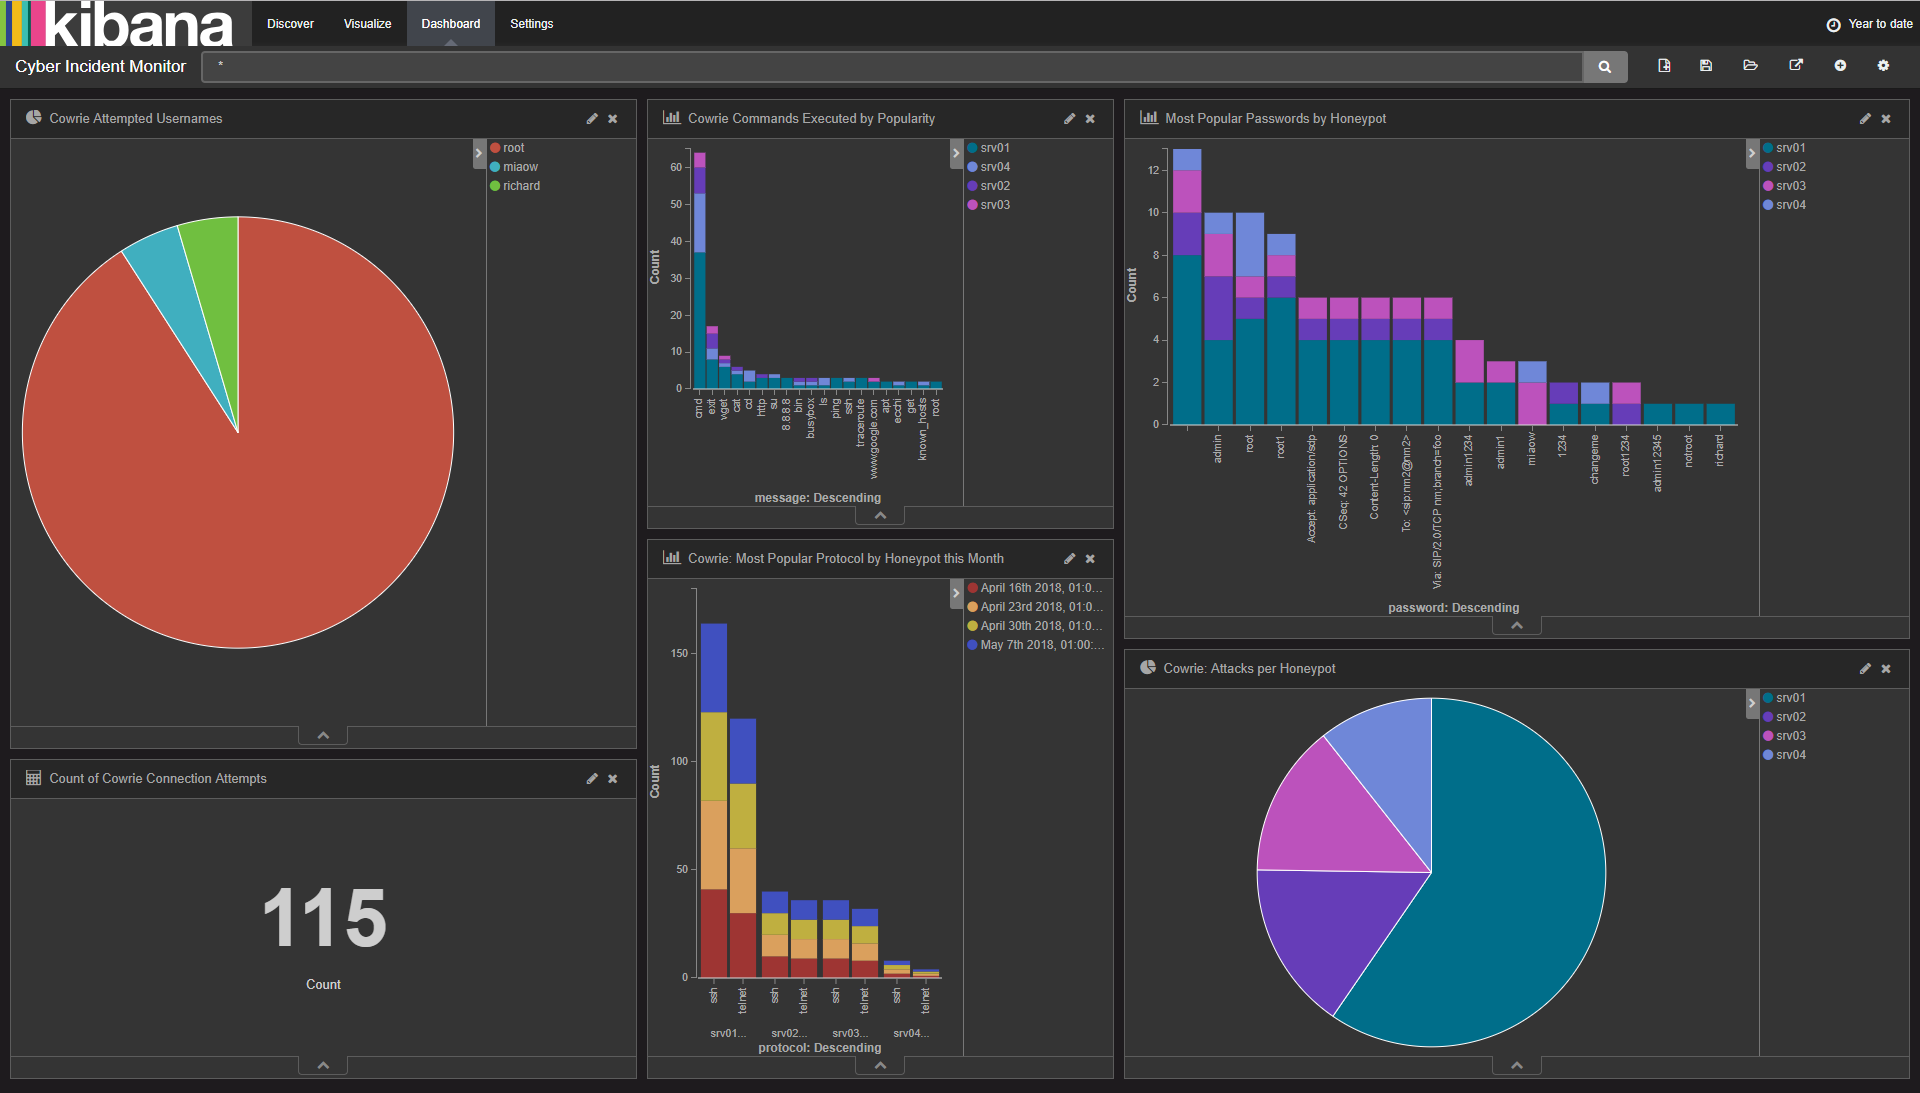
\includegraphics[width=160mm, scale=1]{Images/Some_Cowrie_visualisations_on_the_Kibana_dashboard_.PNG}
      \caption{Cyber Incident Monitor on Kibana} 
      \medskip
      \small
		This image shows the Kibana visualisation dashboard that was created as part of the incident monitoring solution. A number of charts are shown, measuring everything from the popularity of passwords per honeypot to the proportion of telnet and SSH attacks received by each Cowrie honeypot. The dashboard provides a concise description of the threat state of the honeynet.
\label{fig:Some_Cowrie_visualisations_on_the_Kibana_dashboard_.PNG}
\end{figure}

%\includewidefigure{Some_Cowrie_visualisations_on_the_Kibana_dashboard_.PNG}{Cyber Incident Monitor on Kibana}{A collection of visualisation created in Kibana for the cyber-incident monitor.}{Images/Some_Cowrie_visualisations_on_the_Kibana_dashboard_.PNG}

\begin{figure}[ht]
      \centering
      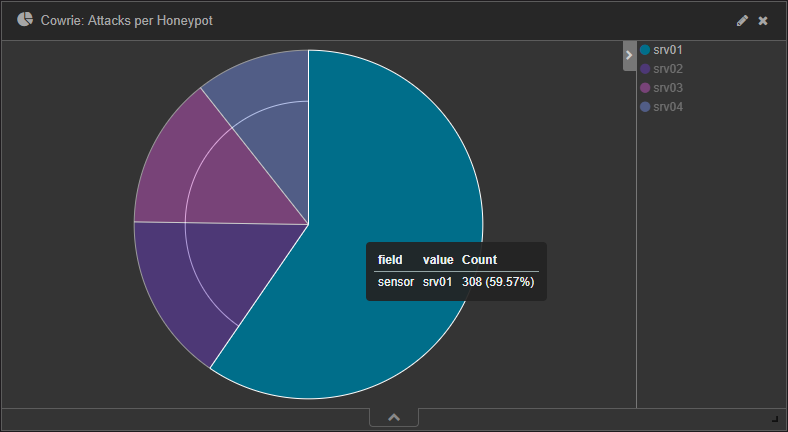
\includegraphics[width=160mm, scale=1]{Images/Cowrie_Attacks_per_honeypot.PNG}
      \caption{Visualisation: Attacks per Honeypot} 
      \medskip
      \small
		This image shows a single visualisation created in Kibana as part of the cyber-incident monitor. This pie-chart shows the proportion of attacks each Cowrie honeypot received within a month.
\label{fig:Cowrie_Attacks_per_honeypot.PNG}
\end{figure}

%\includewidefigure{Cowrie_Attacks_per_honeypot.PNG}{Visualisation: Attacks per Honeypot}{A visualisation created in Kibana as part of the cyber-incident monitor. This pie-chart shows the proportionately how many attacks each honeypot received within a week.}{Images/Cowrie_Attacks_per_honeypot.PNG}

\begin{figure}[ht]
      \centering
      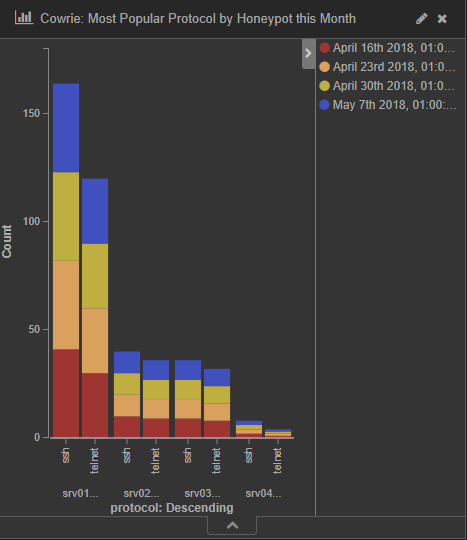
\includegraphics[width=100mm, scale=0.2]{Images/Cowrie_most_popular_protocol_per_honeypot_this_month.PNG}
      \caption{Visualisation: Most Popular Protocols per Honeypot by Month} 
      \medskip
      \small
		This image shows another visualisation created in Kibana as part of the cyber-incident monitor. This chart shows the proportion of SSH and Telnet attacks received by each of the honeypots for each week over the last month.
\label{fig:Cowrie_most_popular_protocol_per_honeypot_this_month.PNG}
\end{figure}

%\includewidefigure{Cowrie_most_popular_protocol_per_honeypot_this_month.PNG}{Visualisation: Most Popular Protocols per Honeypot by Month}{A visualisation created in Kibana as part of the cyber-incident monitor. This chart shows the proportion of SSH and Telnet attacks received by each of the honeypots for each week over the last month.}{Images/Cowrie_most_popular_protocol_per_honeypot_this_month.PNG}

What can be noted about these visualisations is the effectiveness with which information is imparted to the user: Rather than sifting through reams of honeypot log data, correlated information regarding attack behaviours and patterns is represented succinctly in the visualisations. The fact that the logs used to produce these are shipped from the honeypot server approximately every 60 seconds\footnote{As explained in \textit{Section \ref{CRON}}, the honeypot logs were made available to Filebeat every 60 seconds before being shipped to the EC2 management instance. Any additional delay in delivery is likely to be due to network conditions.} means that an administrator is facilitated in understanding the current threats to their system rapidly. 





\subsection{The Design of Adaptive Honeypots}
As such, it would appear that unpredictability is the nature of research where honeypots are involved. It had been hoped that a quantitative evaluation would be provided in this section: However, due to the issues encountered with completing all planned iterations of experiments, the evaluation of the contribution of this research towards the design of adaptive honeypots is restricted by the incomplete results obtained in \textit{Section \ref{ConductingExperiments}}.

\subsubsection{Unpredictability of Honeypot Experiments}
It has been found that the process of designing honeypots to be adaptive to dynamic threats is a time-intensive one. Unforeseen issues such as the requirement to implement a high-interaction container honeypot, and the further significant challenges which were faced in implementing this effectively, are illustrative of the unpredictability of designing adaptive honeypots. 

The fact that the contributions of just 3 characteristics of honeypots were considered in the experiments outlined in \textit{Section \ref{DesignOfExperiments}} is explained by the limited remaining time within which the experiments could be conducted. Had more time been available, a set of comprehensive honeypot experiments could be conducted accounting for several other honeypot characteristics. 

When compared to the time spent conducting similar research experiments in the closely related projects discussed in \textit{Section \ref{CloselyRelatedWork}}, the findings were as follows:
\begin{itemize}
\item The researchers involved in the \textit{IoTPot} project conducted experiments to evaluate the effectiveness of their design in 2 separate phases: a 144-day trial period from 2014/11/07 to 2015/03/31 which was used to ''understand the attackers' behavior and (discuss) the proper setting of the honeypots'', followed by a 28-day stable period from 2015/04/01 to 2015/05/09 in which more structured experiments were conducted. \cite{IoTPot2016}
\item In their evaluation of honeypot performance in the \textit{TraCINg} incident monitor, Vasilomanolakis \textit{et al.} explain that a five-month deployment of their honeypot-driven incident monitor allowed them to obtain meaningful results.  \cite{Vasilomanolakis}
\end{itemize}
These findings further illustrate the unpredictability of evaluating the effectiveness of honeypots. It is perhaps an oversight that the time that would be required to conduct such experiments was not realised at an earlier stage.

In recognition of the fact that none of the experiments conducted could provide \textit{conclusive} evidence regarding the design of adaptive honeypots, there was a need to consider what was (i) necessary, (ii) sufficient and (iii) additional towards the achievement of the original objective.

\begin{enumerate}
\item \textbf{Necessary}

It is necessary that knowledge is gained about the contribution of a honeypot's design to its effectiveness in attracting attacks through experiments. 
\item \textbf{Sufficient}

It is sufficient that the knowledge gained is not conclusive but is based on experimental data.

\item \textbf{Additional}

It is additional that the knowledge gained is definitive and conclusive based on experimental data.

\end{enumerate}
It is clear that obtaining conclusive results regarding effective design for adaptive honeypots  became infeasible because of time constraints, ultimately resulting in the early termination of the experiment phase. However, the data obtained from the three experiment attempts, although not definitive, did provide some insights into the nature of designing adaptive honeypots.
\begin{itemize}
\item The presence of expected utilities and toolkits in a honeypot environment is clearly crucial to its success in encouraging attacks. This was evident from the data captured in attempts 2 and 3 of the experiment iteration performed, where bot attackers did not proceed with compromise of the system when certain utilities were not present in the honeypot environment.
\item Support for protocols and services which are commonly exploited by attackers is an important feature of effective honeypots: this is evident by virtue of the sheer volume of brute-force authentication attacks which were received
\item Basing honeypot design on current knowledge of attacks is a useful starting point in enabling attacks to be studied. In the design of the high-interaction router honeypot, it is likely that the experiments would have been more successful if more emphasis had been placed on configuring the environment to provide responses and utilities sought after by active IoT botnets, knowledge of which already exists in research. \cite{UnderstandingTheMiraiBotnet} \cite{HajimeMysteriousBotnet}
\item Honeypots must be designed to combat both automated and human attackers. It was not expected based on the findings of Barron \textit{et al.} that attacks by human attackers would be likely to be encountered in the honeypot environment. \cite{PickyAttackers2017} The fact an attack session by a human attacker was captured in the limited period for which experiments were conducted illustrates that honeypots should be designed to adapt to threats from human attackers, and not solely the more predictable attack patterns of bots. 
\end{itemize}
\subsubsection{Ability to Capture Attack Data}
As evidenced during the conducting of experiments in \textit{Section \ref{ConductingExperiments}}, the fact that keylogging was not available on the router container honeypot severely limits the conclusions that can be drawn regarding any experimental results that were obtained. For instance, although patterns of command execution were observed in the \textit{.bash\_history}, the lack of timestamping and session IDs for these events meant that inferences were made regarding these sequences being from a single attacker. 

There is plenty of room for improvement regarding the capturing of attack data, and given more time, it would almost certainly be possible to develop an effective and reliable keylogging mechanism for the router container. 

\subsubsection{Hosting Honeypot Experiments on a Cloud Platform}
It is quite probable that some of the attack patterns observed in \textit{Section \ref{ConductingExperiments}} may have been different had a different hosting solution been used to host the system. As noted by Vasilomanolakis \textit{et al.} in their implementation of a honeypot incident monitor, \cite{Vasilomanolakis} many cloud service providers publish their IP ranges on the public internet: AWS is one such provider. \cite{AWS_PublicIPRanges} In their paper examining the difference between human and automated attacks, Barron \textit{et al.}  also find that ''location and host matters... if someone is operating on a constrained budget and wants to maximize the number of brute-forcing IP addresses collected, AWS appears to be the infrastructure that will facilitate this''. \cite{PickyAttackers2017}

As AWS are a very well-known and popular cloud hosting provider, they are likely an attractive target for attackers who have knowledge of their public IP ranges. Thus, there is potential for some bias in results obtained in a deployment such as that implemented in this research, where all honeypots are hosted in a single geographical region by a single hosting provider. 
 
%Allowing IoT bot attackers to authenticate easily is important, so supporting as many username-password combinations as possible is a good idea. This is in line with what was found by the IoTPot researchers. \cite{IoTPot2016}
%Providing the utilities that the attacker expects to find is also important, since it was ultimately issues like this that resulted in repeating the first experiment.
%High-interaction IoT honeypots take a lot of maintenance


\subsubsection{Fingerprinting Container Environments}
An interesting observation regarding the fingerprinting of honeypot environments is that there are many ways in which an attacker can detect that they are inside a container, if the honeypot is indeed the container itself. This was noted during the implementation of the system, when the command \textit{cat /proc/1/cgroup} was executed, leading to the output shown in figure \ref{fig:DockerFingerprintingCommand}. This is consistent with the findings of Kedrowitsch \textit{et al.} when evaluating the suspectibility of containers to being fingerprinted. \cite{LXCsForDeceptiveHoneypots2017}

\begin{figure}[ht]
      \centering
      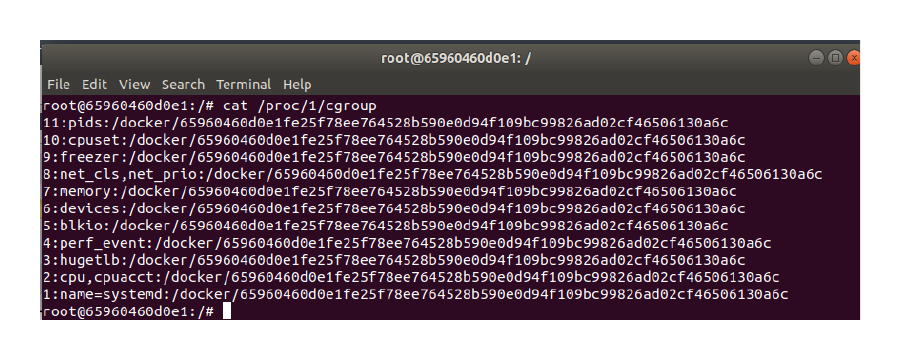
\includegraphics[width=160mm, scale=1]{Images/Fingerprinting_Docker_Containers__1_.png}
      \caption{Fingerprinting of Docker Environments} 
      \medskip
      \small
		This console output was generated as a result of executing the command \textit{cat /proc/1/cgroup} inside the router container. It clearly includes several references to 'docker', which any attacker aware of Docker would immediately recognise as being a container environment.
\label{fig:DockerFingerprintingCommand}
\end{figure}

%\includewidefigure{DockerFingerprintingCommand}{Fingerprinting of Docker Environments}{This console output was generated as a result of executing the command \textit{cat /proc/1/cgroup}. It clearly includes several references to 'docker', which any attacker aware of Docker would immediately recognise as being a container environment.}{Images/Fingerprinting_Docker_Containers__1_.png}

This may not come as a surprise to an attacker: As organisations increasingly include containers as part of their infrastructure, this information would likely not identify the container as being a honeypot. However, it is certainly worth considering that if containerised honeypots begin to be used more widely, fingerprinting of these systems as honeypot environments may also become more common. 


\section{Summary} \label{SummaryOfChapter6}

It is clear that the unpredictability of conducting honeypot experiments was a barrier to obtaining measurable data and providing definitive conclusions regarding the adaptive design of honeypots. This was largely an oversight in the design phase of the research, where had more time been available, there would have been a greater opportunity to achieve this objective as part of this research.

However inconclusive, useful insights have been obtained from the experiments conducted. This is an encouraging indication of the potential for a real contribution to be made through experiments of this nature, and provides a strong basis for completing the remaining iterations of the project as future work. 			%% EVALUATION
\chapter{Conclusions and Future Work} \label{Chapter7}
The objectives set out for this research in \textit{Section \ref{ProposedWork}} of this document, although not achieved fully, yielded enhancements to the deployability of active network defence through incident monitoring as well as valuable insights into the way in which such systems should be designed to improve their threat detection capabilities.

Section \ref{ConclusionsSection} draws some conclusions regarding the outcomes of the research, focusing on the original elements of the research objectives.

Section \ref{FutureWork} explores a number of potential avenues for expanding upon the research conducted in this project. These include potential improvements to the proposed approach as well as opportunities to conduct additional work building on the foundations laid by this research.

Finally, \textit{Section \ref{FinalRemarks}} includes some final remarks and recommendations based on the research conducted.

%
% CONCLUSIONS
% 
\section{Conclusions} \label{ConclusionsSection}
Though it is clear that this research would have benefited significantly from additional time within which to meet its objectives, the substantiality of knowledge gained from the exploration of challenges in the field of security today was unprecedented.

The major achievements and conclusions drawn from this research are described in the following subsections.

\subsection{Cyber Incident Monitoring in Critical Infrastructures}
The major contribution of this work has been the development of a novel containerised honeynet-driven incident monitor. The value that can be provided by the succinct description of attack data through visualisation is evident: These incident monitors allow system administrators to represent threat data in a meaningful way, enabling a holistic view of their systems.

There is tangible evidence that the incident monitor developed in this research provides greater usability of honeypot data than that which would have resulted from just using honeypots alone:

\begin{itemize}

\item Visualisation of the honeypot data means that reams of logs don't have to be searched through in order to understand the most relevant threat information;
\item The aggregation of data from multiple honeypots by a centralised logging system, allowing trends to be easily identified;
\item The ability to receive instantaneous threat intelligence alerts via email, pin-pointing the perpetrator;
\item The fact that installation and configuration of the honeypots is automated, as well as the networking required to connect them.
\end{itemize}

As such, this development has effectively addressed many of the major barriers to employing active network defence in infrastructures today: A valuable contribution to the field of security.

\subsection{The Potential of Containers for Security Applications}
The use of containers has added substantial value to the honeynet solution implemented in this project. It serves as a proof-of-concept with regards to usability of active network defence mechanisms for network administrators by providing the ability to automatically install and configure multiple replicable environments on-the-fly.

As evidenced by this research, the work being done to containerise security applications is something that presents many challenges: There are no manuals or existing resources to refer to in the development of such systems, and so there is a lot of room for research and evaluation of different approaches to doing so.

\subsection{The Importance of Honeypots in Active Network Defence}
As has been observed during the course of this research, working with honeypots can be highly unpredictable, making conclusive research difficult to achieve under time constraints. However, it is clear that the ability of honeypots to provide active network defence through deceiving and monitoring attackers make them an attractive option for combating the dynamic, evolving threats that are increasingly impacting individuals and organisations across the world. Critical service infrastructures are in desperate need of the \textit{adaptive} threat detection capabilities of honeypots to protect their systems and those who depend on them.

\subsection{The Future of IoT Security}

It is clear even from the limited experiments that were conducted in this research that IoT botnets are extremely active: Every ''thing'' with internet connectivity is a means of exploiting communications and interaction. People are increasingly dependent on interconnected services and applications, and as a result are vulnerable to cyber threats beyond the reach of their own devices. 

Critical service architectures will continue to be targeted by severe cyber attacks well into the future as nation states continue to engage in cyber-combat. There will need to be huge innovation in the area of IoT security before the gargantuan challenges being faced by these infrastructures can even be remotely resolved: It is only when a system is designed with security in mind that a system can be considered even relatively secure. Applications are continuing to have connectivity integrated into them with very little consideration given to their security, and this is something that is not likely to end any time soon. It is likely that until there is a truly market-driven incentive for manufacturers to implement decent security mechanisms in their products, this is unlikely to change.


%
% FUTURE WORK
% 
\section{Future Work} \label{FutureWork}
Whilst an end-to-end cyber incident monitoring system was successfully developed in this research, the full intended evaluation of the system was not possible as discussed in \textit{Section \ref{DesignPivot1}}. However, this gives rise to opportunities for additional developments and enhancements based on the foundations laid by this research, a number of which are discussed below.


\subsection{Extension of the Cowrie Honeypot} \label{ExtendingCowrie}

As explained in the \textit{Section \ref{DesignPivot1}}, the Cowrie honeypot by design does not allow outbound network connections. This research would have benefited greatly from the extension of the Cowrie honeypot to include this functionality, but time constraints meant that such a development was not within the scope of the project. 

Though an in-depth inspection of how such an extension could be added to the Cowrie source code was not conducted, it is clear that it would involve relatively significant development effort to implement an additional networking client as part of the Cowrie application in Python. The Cowrie application already includes Python modules for SSH and telnet traffic forwarding which would form a useful starting point in this implementation.

Such a networking client would need to be able to have a view of the underlying networking stack of the host, such that outbound connections to other Cowrie honeypots can be facilitated and a view of hosts nearby can be obtained so that an attacker is not expected to probe IP address ranges blindly. However, the addition of outbound networking capabilities in the Cowrie honeypot would bring it closer to becoming a high-interaction honeypot, which creates a number of new issues for the use of Cowrie. Circumventing the risks associated with high-interaction honeypots is challenging, as was found during this project.
\begin{itemize}
\item The networking client would need to implement some destination authentication mechanism such that outbound connections from Cowrie are only permitted to other Cowrie honeypots. This would minimise the risk of a Cowrie honeypot propagating an attack to another Cowrie honeypot;
\item The interface between the networking client and the network stack of the host system would need to be very carefully implemented and audited for it to be shipped as part of the Cowrie honeypot package, since it should be very difficult for an attacker to exploit such an interface to the host system.
\end{itemize}

The addition of this feature as an optional function of the Cowrie honeypot would facilitate the future deployment of honeynets entirely based on the Cowrie honeypot, leveraging all of its configuration and logging capabilities. This would be a very useful contribution to the Cowrie development effort, and would be an excellent starting point for a continuation of the work conducted in this research.


%\subsection{%Alternative Network Configurations}
%Multiple honeynets connected to the single router? (Maybe with fewer honeypots per net)

\subsection{An Improved High-Interaction Containerised Honeypot}
It is clear from the challenges encountered in both the implementation of the incident monitor and the experiments to determine an effective design for adaptive honeypots, that the router container honeypot left much to be desired in terms of its ability to facilitate attacks. This is largely due to the fact that this honeypot was not included as an original component of the proposed system, and so did not benefit from the substantially greater consideration of related literature that preceded the design of other components of the system.

There is much opportunity for improvement of the router container honeypot. There were no existing container-based high interaction honeypots found during the course of this research, a gap which many would benefit from being filled.

Some potential areas for improvement of the existing router honeypot that have been identified include the following:
\begin{itemize}
    \item Further isolation from the host system through investigation of alternative Docker networking approaches;
    \item The implementation of reliable, detailed keylogging inside the router container that could be used to visualise the commands executed by attackers;
    \item Extension of the image definition of the router honeypot to target requirements of specific IoT botnets, rather than solely improving the design by incrementally altering the environment on an experiment-by-experiment basis. 
\end{itemize}

Given these improvements and sufficient time, it would be strongly recommended that the experiment iterations or an extension of these should be resumed in a bid to improve upon the current state-of-the-art in adaptive honeypots. It is however strongly recommended that any future work conducted into experiment-based design of honeypots should consider the unpredictability factor associated with such work during the design phase.


\subsection{Machine Learning Approaches to Adaptive Honeypot Design}
There is huge potential for the implementation of machine learning-based honeypot solutions, similar to that developed by the researchers behind IoTCandyJar. \cite{IoTCandyJar} The use of such techniques enables honeypots to self-improve by learning what makes them most effective in enticing and maintaining the interest of attackers, making for ultimately more effective active defence in networks.

In the context of the work that has been done in this project towards proposing design approaches for adaptive honeypots, a machine learning back-end component similar to the \textit{IoTLearner} module implemented by the IoTCandyJar researchers would be an excellent enhancement to the system that has been developed. \cite{IoTCandyJar} Such a module could potentially perform many of the functions currently performed by the router honeypot, providing responses that would encourage the attacker to progress their attack to the stage that they would look to propagate it to nearby hosts. To enable this propagation would either require:
\begin{itemize}
\item A traffic routing module similar to that proposed in \textit{Section \ref{ExtendingCowrie}} to route SSH and telnet attack traffic to the Cowrie honeynet; or
\item An architecture similar to that proposed by the IoTPot researchers, where the \textit{IoTLearner} machine learning module would act as the \textit{front-end responder} in the IoTPot architecture and forward connection requests to a high-interaction backend to be handled. \cite{IoTPot2016} \cite{IoTCandyJar} 
\end{itemize}

In summary, the use of machine learning approaches in the implementation of dynamic, reactive honeypots coupled with the novel architecture and deployability of the incident monitoring solution developed in this research would be a very worthwhile investment as a future project.


 
\subsection{Alternative Threat Notification Systems}
The alert generation system that was used in this project was the commonly used port scan detection tool PSAD. It was found to effectively detect probing of the EC2 honeypot instance on which the containerised honeypot was hosted, generating email alerts for any probes detected almost instantaneously. However, it was also relatively prone to generating false positives because of scenarios such as that described in \textit{Section \ref{AlertSystemSection}}.

There is certainly potential for other alerting mechanisms to be used in this system which may provide more accurate and effective communication of threat intelligence. Of note is the fact that the Cowrie project supports integration with Slack, an instant messaging and collaboration service that is used in many organisations for workplace communication. As a system that can provide instant messages to a distributed set of mobile users, there is potential for the use of Slack and similar messaging channels as a means of providing threat intelligence alerts generated by the Cowrie honeynet.

\subsection{Alternative System Architectures \label{AlternativeSystemArchitectureFW}}
 As identified in \textit{Section \ref{CentralisedManagementEvaluation}}, the fact that there is only a single management server supporting the processing and visualisation of all of the honeypot log data means that there is a single point of failure in the system. Should the management instance crash due to any system failure, the entire incident monitoring system would not be available to provide analysis and visualisation of attack data.
 
More distributed approaches such as passive replication could provide greater reliability for the system: By passively replicating the management instance, there would always be a node capable of processing honeypot logs and providing visualisations to system administrators. This would incur significant initial configuration overhead: An initial estimation of effort involved here for a single replica would include:
\begin{itemize}
\item The provision of a new EC2 instance capable of hosting the ELK log processing stack;
\item Replicated configuration of the ELK stack tools and Nginx on the new EC2 instance;
\item The generation and distribution of an additional SSL certificate to the EC2 honeypot instance;
\item Updating the configuration of Filebeat to ship honeypot logs to both server instances;
\item The addition of a monitoring communication between the two management servers, such that the passive replica can take over if the primary fails.
\end{itemize}

In addition, ongoing maintenance overheads must be considered by virtue of the addition of another node to the system. However, adding replication would significantly increase the reliability of what is a time-sensitive threat mitigation service.


%
% CLOSING REMARKS
% 
\section{Closing Remarks} \label{FinalRemarks}
%  in a way that caters for the stringent requirements of a production network
This research has seen the development of a containerised cyber-incident monitor: A proposal to address the need for active defence mechanisms in systems of critical services. Though there is significant work remaining to make this system production-ready, there are many elements of the proposed system which address the current issues being faced in these infrastructures by providing a feasible, flexible active defence solution.

Active network defences with their ability to adapt to detect new threats will only become more important into the future as the gap between threats and the mitigations against them continues to widen. There is a fundamental shift in outlook required by those managing the security of IT systems, such that preventative security measures are not the sole mechanisms protecting them from increasingly sophisticated threats.

The crucial takeaway from this research is that it is of critical importance in the development of any software system that a threat model is included in the design from the very beginning. If this is widely included as part of software design and implementation, it is likely that more risks will be mitigated and that fewer  vulnerabilities will arise. Though it is only theoretically possible to evaluate and eradicate \textit{all} vulnerabilities in a system, a security-oriented approach to designing software systems would go a long way towards reducing the implications of serious attacks on their users.
				%% CONCLUSION

\begin{appendix}
\chapter{Abbreviations} \label{Abbrevations}

\begin{tabular}{p{40mm}|p{100mm}}
	\textbf{Abbreviation}&\textbf{Expanded Term}\\
	\hline
	ACK&Acknowledgement\\
    API&Application Programming Interface\\
    AWS&Amazon Web Services\\
    C+C&Command and Control\\
    CLI&Command Line Interface\\
    CRON&Command Run-ON\\
    DoS&Denial of Service\\
    DDoS&Distributed Denial of Service \\
    DMZ&De-Militarised Zone\\
    DNS&Domain Name System\\
    DPI&Deep-Packet Inspection\\
    DVR&Digital Video Recorder\\
    EC2&Elastic Compute Cloud (AWS)\\
	ELK&Elasticsearch-Logstash-Kibana Stack\\
    FTP&File Transfer Protocol\\
    %GW&Gateway (Network)\\

\end{tabular}    

\begin{tabular}{p{40mm}|p{100mm}}
	\textbf{Abbreviation}&\textbf{Expanded Term}\\
	\hline
    HTTP&Hypertext Transfer Protocol\\
    IaaS&Infrastructure as a Service\\
    ICMP&Internet Control Message Protocol\\
    IDS&Intrusion Detection System\\
    IETF&Internet Engineering Task Force\\
    IoT&Internet of Things\\
    IP&Internet Protocol\\
    IT&Information Technology\\
    JSON&JavaScript Object Notation\\
    LPWAN&Low-Powered Wide-Area Network\\
    LXC&Linux Container\\
    MHN&Modern Honey Network\\
    NAT&Network Address Translation\\% TODO ensure this is mentioned in the router configuration description
    NHS&National Health Service, UK\\
    NTP&Network Time Protocol\\
    OS&Operating System\\
    %P2P&Peer-to-Peer\\
    PaaS&Platform as a Service\\
    PSAD&Port Scan Attack Detection\\
    RAM&Random Access Memory\\
    RCE&Remote Code Execution\\
    RSA&Rivest, Shamir, and Adelman\\
    SAN&SubjectAltName field of SSL certificate\\
    SANS&System Administration, Networking, and Security Institute\\
    SCADA&Supervisory Control and Data Acquisition\\ 
    SCP&Secure Copy\\

    \end{tabular} 

\begin{tabular}{p{40mm}|p{100mm}}
	\textbf{Abbreviation}&\textbf{Expanded Term}\\
	\hline
    SHA&Secure Hash Algorithm\\
    SMB&Server Message Block\\
    SMTP&Simple Mail Transfer Protocol\\
    SNMP&Simple Network Management Protocol\\
    SSH&Secure SHell\\
    SSL&Secure Sockets Layer\\
    TCP&Transmission Control Protocol\\
    TFTP&Trivial File Transfer Protocol\\
    TLS&Transport Layer Security\\
    VM&Virtual Machine\\
	WSN&Wireless Sensor Network\\
    YAML&Yet Another Markup Language\\
\end{tabular} 
						%% ABBREVIATIONS
\end{appendix}


%
\bibliographystyle{ieeetr}
\bibliography{dissertation}                      
%\addcontentsline {toc}{chapter}{Bibliography}     %% Force Bibliography to appear in contents


\end{document}                             %% END THE DOCUMENT